\documentclass[a4paper, 9pt]{scrartcl}\usepackage[]{graphicx}\usepackage[]{xcolor}
% maxwidth is the original width if it is less than linewidth
% otherwise use linewidth (to make sure the graphics do not exceed the margin)
\makeatletter
\def\maxwidth{ %
  \ifdim\Gin@nat@width>\linewidth
    \linewidth
  \else
    \Gin@nat@width
  \fi
}
\makeatother

\definecolor{fgcolor}{rgb}{0.345, 0.345, 0.345}
\newcommand{\hlnum}[1]{\textcolor[rgb]{0.686,0.059,0.569}{#1}}%
\newcommand{\hlstr}[1]{\textcolor[rgb]{0.192,0.494,0.8}{#1}}%
\newcommand{\hlcom}[1]{\textcolor[rgb]{0.678,0.584,0.686}{\textit{#1}}}%
\newcommand{\hlopt}[1]{\textcolor[rgb]{0,0,0}{#1}}%
\newcommand{\hlstd}[1]{\textcolor[rgb]{0.345,0.345,0.345}{#1}}%
\newcommand{\hlkwa}[1]{\textcolor[rgb]{0.161,0.373,0.58}{\textbf{#1}}}%
\newcommand{\hlkwb}[1]{\textcolor[rgb]{0.69,0.353,0.396}{#1}}%
\newcommand{\hlkwc}[1]{\textcolor[rgb]{0.333,0.667,0.333}{#1}}%
\newcommand{\hlkwd}[1]{\textcolor[rgb]{0.737,0.353,0.396}{\textbf{#1}}}%
\let\hlipl\hlkwb

\usepackage{framed}
\makeatletter
\newenvironment{kframe}{%
 \def\at@end@of@kframe{}%
 \ifinner\ifhmode%
  \def\at@end@of@kframe{\end{minipage}}%
  \begin{minipage}{\columnwidth}%
 \fi\fi%
 \def\FrameCommand##1{\hskip\@totalleftmargin \hskip-\fboxsep
 \colorbox{shadecolor}{##1}\hskip-\fboxsep
     % There is no \\@totalrightmargin, so:
     \hskip-\linewidth \hskip-\@totalleftmargin \hskip\columnwidth}%
 \MakeFramed {\advance\hsize-\width
   \@totalleftmargin\z@ \linewidth\hsize
   \@setminipage}}%
 {\par\unskip\endMakeFramed%
 \at@end@of@kframe}
\makeatother

\definecolor{shadecolor}{rgb}{.97, .97, .97}
\definecolor{messagecolor}{rgb}{0, 0, 0}
\definecolor{warningcolor}{rgb}{1, 0, 1}
\definecolor{errorcolor}{rgb}{1, 0, 0}
\newenvironment{knitrout}{}{} % an empty environment to be redefined in TeX

\usepackage{alltt}
\usepackage[ngerman]{babel}

% -----------------------------------------------------------------------

% -----------------------------------------------------------------------
%% ------------------------------------------------------------
%% by J.Kruppa on Friday, February 11, 2022 (11:31)
%% \def\mainDir{\Sexpr{exam_path}}
\def\source{/Users/jokruppa/source/tex}
\usepackage[margin=2cm, includefoot]{geometry}
\setlength{\parindent}{0cm}
\usepackage{booktabs}
\usepackage{amsmath}
\usepackage{scalerel,amssymb}
\usepackage{setspace}
\def\csquare{{\Large $\boxtimes$}}
\def\msquare{{\Large $\square$}}
\usepackage[normalem]{ulem}
\usepackage{array}
\usepackage{xcolor}
\usepackage{float}
\usepackage{currfile}
\usepackage{tikz}
\usepackage[nomessages]{fp}

%% beamer defs
\def\lecture{Klausurfragen der Bio Data Science}

%% exam defs
\def\examtitle{\lecture}
\def\exammodule{
\vspace{-1.75cm}  
\begin{graybox}{}
\vspace{2Ex}
\textbf{\large Name:} \rule[0ex]{16.75em}{.4pt}
\hfill \textnormal{\textit{Nicht bestanden:}} \msquare \\[2.5Ex]
\textbf{\large Vorname:} \rule[0ex]{15em}{.4pt} \\[2.5Ex]
\textbf{\large Matrikelnummer:} \rule[0ex]{10.8em}{.4pt}
\hfill Endnote: \rule[0ex]{7em}{.4pt} 
\end{graybox}
\vspace{3Ex}
\phantom{text}
}
\def\examsemester{Sommersemester \& Wintersemester}
\def\examdate{\today}
%% ------------------------------------------------------------
\definecolor{darkblue}{rgb}{0,0,.5}
\definecolor{darkpurple}{rgb}{0.4117, 0.2, 0.4117}
\definecolor{uni}{rgb}{0,0.3137,0.6078}
\definecolor{gray}{gray}{0.7}

\usepackage{tcolorbox}
\definecolor{logo1}{RGB}{0, 158, 227}
\definecolor{gray5}{RGB}{247, 247, 247}
\definecolor{gray2}{RGB}{102, 102, 102}

\newtcolorbox{graybox}[1]{
  colback=gray5,%%red!5!white,
  colframe=gray2,%%red!75!black,
  fonttitle=\bfseries\Large,
  %%valign=center,
  fontupper=\large,
  before skip=10pt plus 2pt,
  after skip=20pt plus 4pt,
  title=#1}

\newtcolorbox{takehomebox}[1]{
  colback=gray5,%%red!5!white,
  colframe=logo1,%%red!75!black,
  fonttitle=\bfseries\Large,
  %%valign=center,
  fontupper=\large,
  before skip=10pt plus 2pt,
  after skip=10pt plus 2pt,
  title=#1}

\def\Rlogo{
\includegraphics[width = 0.5cm]{\string~/Documents/GitHub/exam/img/Rlogo}\;}

\usepackage[scaled=.90]{helvet} 
\usepackage{fancyhdr}
\usepackage{lastpage}
\usepackage{hyperref}
\hypersetup{
    colorlinks=true,       % false: boxed links; true: colored links
    linkcolor=black,          % color of internal links 
    urlcolor=magenta           % color of external links
}
\renewcommand{\familydefault}{\sfdefault}

\title{
\large \exammodule \\[5Ex]
\Huge \examtitle \\[2Ex] 
\Large Hochschule Osnabr{\"u}ck
}
\author{Pr{\"u}fer: Prof. Dr. Jochen Kruppa \\
Fakult{\"a}t f{\"u}r Agrarwissenschaften und Landschaftsarchitektur \\ 
j.kruppa@hs-osnabrueck.de}
\date{Version vom \examdate}

%% ------------------------------------------------------------
%% by J.Kruppa on Tuesday, September 23, 2014 (12:50)
%% Header
\renewcommand{\headrulewidth}{0pt}
\renewcommand{\footrulewidth}{0pt}
\pagestyle{fancy}

\fancyhf{}
\fancyhead[L]{}
\fancyhead[R]{}
\fancyfoot[R]{\thepage}
\fancyfoot[L]{\footnotesize \examtitle}

\fancypagestyle{empty}{
 \fancyhf{}
 \fancyhead[L]{}
 \fancyhead[R]{}
 \fancyfoot[R]{\thepage}
 \fancyfoot[L]{\footnotesize \examtitle}
}

\usepackage{arevtext,arevmath}

\newcommand\Tstrut{\rule{0pt}{2.6ex}}         % = `top' strut
\newcommand\Bstrut{\rule[-0.9ex]{0pt}{0pt}}   % = `bottom' strut
\def\strut{\Tstrut\Bstrut}

% -----------------------------------------------------------------------
\IfFileExists{upquote.sty}{\usepackage{upquote}}{}
\begin{document}
\date{Wintersemester 2024/25 
\vfill
\begin{center}

\includegraphics[width = 1.9cm]{avatare/Alex}\hspace{-8mm}

\includegraphics[width = 1.9cm]{avatare/Jessica}\hspace{-8mm}

\includegraphics[width = 1.9cm]{avatare/Jonas}\hspace{-8mm}

\includegraphics[width = 1.9cm]{avatare/Mark}\hspace{-8mm}

\includegraphics[width = 1.9cm]{avatare/Nilufar}\hspace{-8mm}

\includegraphics[width = 1.9cm]{avatare/Paula}\hspace{-8mm}

\includegraphics[width = 1.9cm]{avatare/Steffen}\hspace{-8mm}

\includegraphics[width = 1.9cm]{avatare/Tina}\hspace{-8mm}

\includegraphics[width = 1.9cm]{avatare/Yuki}\\
\small
\vspace{1.5Ex}
\textit{"`The test of a student is not how much he knows,\\ but how much he wants to know."'\\ --- Alice W. Rollins}
\end{center}}
% -----------------------------------------------------------------------
\maketitle
\fancypagestyle{empty}{
  \fancyfoot[L]{\tiny $\square\!\blacksquare\!\blacksquare\!\square\!\square\!\square\!\square\!\blacksquare\!\blacksquare\!\square\!\blacksquare\!\blacksquare\!\blacksquare\!\blacksquare\!\blacksquare\!\blacksquare\!\blacksquare\!\square\!\blacksquare\!\blacksquare$}
}
\thispagestyle{empty}
\clearpage
% -----------------------------------------------------------------------
\begin{minipage}[c]{0.125\textwidth}

\includegraphics[width = 1.9cm]{avatare/Alex}
\end{minipage}
\begin{minipage}[c]{0.875\textwidth}
\textit{Alex studiert im 3. Semester und wiederholt das Modul, da er im ersten Jahr andere Prioritäten für sich gesetzt hat. Das musste sein, da er sich ziemlich im Abitur verausgabt hat. Darüber hinaus war die WG auch eher auf Party angelegt. Alex hofft jetzt über Pünktlichkeit wieder in die Bahn zu kommen. Dafür steht er jetzt immer um 5 Uhr auf! Freunde von ihm beschreiben ihn eher als extrovertiert. Er kennt Paula noch aus der Schulzeit und er überlegt, ob nicht beide Mal nach Mallorca sollten.} 
\end{minipage}\\[2.75Ex]
% -----------------------------------------------------------------------
\begin{minipage}[c]{0.875\textwidth}
\textit{Nach zwei Semestern Studium an der Universität Osnabrück war es dann Jessica doch viel zu theoretisch. Etwas angewandtes sollte es sein, wo sie auch eine Fähigkeit lernt, die frau nutzen kann. Deshalb hat sich Jessica an der Hochschule eingeschrieben. Hoffentlich lernt sie etwas nützliches, wo andere für Geld geben würden. Wer nützlich ist, ist wertvoll. Ihr Traum ist ja eine Hundeschule aufzumachen. Die großen Parties hat sie immer gemieden. Sie ist lieber mit ihrer Hündin im Teuteburgerwald.}
\end{minipage}
\begin{minipage}[c]{0.125\textwidth}

\includegraphics[width = 1.9cm]{avatare/Jessica}
\end{minipage}\\[2.75Ex]
% -----------------------------------------------------------------------
\begin{minipage}[c]{0.125\textwidth}

\includegraphics[width = 1.9cm]{avatare/Jonas}
\end{minipage}
\begin{minipage}[c]{0.875\textwidth}
\textit{Das ist jetzt der letzte Versuch mit einem Studium. Wenn es nicht klappt dann überlegt Jonas das \href{https://www.ihk.de/osnabrueck/aus-und-weiterbildung/ausbildung/ausbildungsbetriebe/projekt-neustart-1087206}{Programm der IHK zu Ausbildungsvermittlung} zu nutzen. Aber eine Runde gibt er sich noch. Struktur ist eigentlich das Wichtigste und diesmal hat er sich alle Altklausuren der Fachschaft besorgt. Dann ist er auch noch gleich der Fachschaft beigetreten um mehr Informationen abzugreifen. Und er versucht nicht seine Zeit mit Alex zu verdaddeln oder in der Fachschaft bei einem Bier oder so...}
\end{minipage}\\[2.75Ex]
% -----------------------------------------------------------------------
\begin{minipage}[c]{0.875\textwidth}
\textit{Nächstes Semester geht es nach Kanada davon hat er schon auf der Berufsschule geträumt. Deshalb konzentriert er sich sehr auf die Prüfungen. Ein Schiff ist im Hafen sicher, aber dafür ist es nicht gebaut worden. Das \href{https://www.hs-osnabrueck.de/wir/fakultaeten/aul/international/}{International Faculty Office} der Fakultät Agrarwissenschaften und Landschaftsarchitektur hat super geholfen, aber es waren einiges an Unterlagen. Jetzt hofft er, dass Tina dann doch noch mitkommt. Aber sonst macht er das eben alleine. Obwohl das eher nicht so seine Art ist. Vielleicht sollte er sich mal einen Tipp bei Tina holen, sie wirkt sehr entschlossen.} 
\end{minipage}
\begin{minipage}[c]{0.125\textwidth}

\includegraphics[width = 1.9cm]{avatare/Mark}
\end{minipage}\\[2.75Ex]
% -----------------------------------------------------------------------
\begin{minipage}[c]{0.125\textwidth}

\includegraphics[width = 1.9cm]{avatare/Nilufar}
\end{minipage}
\begin{minipage}[c]{0.875\textwidth}
\textit{Nach der Ausbildung wollte Nilufar eigentlich gleich anfangen zu arbeiten, aber nach einem Praktikum und der Probezeit stellte sie fest, dass es ohne einen Hochschulabschluss schwer wird Führungsverantwortung zu übernehmen. Mit Menschen kann sie schon immer und dann auch eigene Projekte mit anderen verwirklichen, dass ist doch was. Mit dem notwendigen Abschluss sollte der Start um so einfacher sein. Dann ist sie keine Befehlsempfängerin mehr sondern gibt die Marschrichtung vor. Schon jetzt koordiniert Nilufar das Studium von anderen.}
\end{minipage}\\[2.75Ex]
% -----------------------------------------------------------------------
\begin{minipage}[c]{0.875\textwidth}
\textit{Paula möchte die Welt zu einem besseren Ort machen. Wenn da nicht die anderen Mitmenschen wären. Paula muss das Modul nochmal wiederholen, da es dann am Ende des Semesters zu viel für sie wurde. Eine Lerngruppe hätte geholfen, aber das ist dann gar nicht so einfach eine zu finden. Zwar kennt sie schon Nilufar, aber Nilufar ist ihr manchmal zu forsch. Ihr schwant aber, dass alleine das Studium sehr schwer werden wird. Das Abitur war schon so ein Lernhorror, das möchte sie nicht nochmal. Alex sieht sie da als Vorbild.}
\end{minipage}
\begin{minipage}[c]{0.125\textwidth}

\includegraphics[width = 1.9cm]{avatare/Paula}
\end{minipage}\\[2.75Ex]
% -----------------------------------------------------------------------
\begin{minipage}[c]{0.125\textwidth}

\includegraphics[width = 1.9cm]{avatare/Steffen}
\end{minipage}
\begin{minipage}[c]{0.875\textwidth}
\textit{Sommer, Sonne, Natur. Das ist es was Steffen mag. Raus in die Komune und die Natur genießen. Leider hat Steffen noch andere Bedürfnisse, die ein Einkommen benötigen. Da Studierte mehr verdienen, würde dann in Teilzeit auch mehr rausspringen. Wenn er dann privat was anbauen kann, dann spart er gleich doppelt. Leider sind viele seiner Kommilitonen total verkrampfte Karrieristen. Es geht nur ums Äußere. Dabei verliert sich Steffen gerne im Prozess. Das hat auch seinen Schulabschluss etwas verzögert. Steffen lässt sich eben Zeit.}
\end{minipage}\\[2.75Ex]
% -----------------------------------------------------------------------
\begin{minipage}[c]{0.875\textwidth}
\textit{Wille  war es, die es Tina hierher gebracht hat und Wille wird es sein, die Tina dann auch zum Abschluß treibt. Nach einem Rückschlag muss Tina jetzt einige Module wiederholen, damit sie dann auch fertig wird. Ab und zu ist sie schwach gewesen und das hat dann Zeit gekostet. Das Tina es dann manchmal übertreibt, weiß sie nur zu gut, aber irgendwie muss die Kontrolle ja erhalten bleiben? Insbesondere, wenn sie mal wieder die Nacht durchgefeiert hat, verachtet Tina sich. Dann baut Nilufar sie dann bei einem Tee wieder auf.}
\end{minipage}
\begin{minipage}[c]{0.125\textwidth}

\includegraphics[width = 1.9cm]{avatare/Tina}
\end{minipage}\\[2.75Ex]
% -----------------------------------------------------------------------
\begin{minipage}[c]{0.125\textwidth}

\includegraphics[width = 1.9cm]{avatare/Yuki}
\end{minipage}
\begin{minipage}[c]{0.875\textwidth}
\textit{Für Yuki war es nicht einfach. Teilweise war die Krankheit sehr hinderlich, dann war es Yuki selber. Dann muss man auch wieder auf die Beine kommen und es dauert eben seine Zeit. Aber immerhin hat Yuki es jetzt den Abschluss gekriegt und hat einen Studienplatz. Jetzt heißt es in den Rhythmus kommen und schauen, was noch so passiert. Immerhin hat Yuki schon eine kleine Gruppe gefunden, in der Yuki dann Hilfe findet. Ist aber auch sehr unübersichtlich so ein Studium. Steffen ist immer super entspannt.}
\end{minipage}
\clearpage
% -----------------------------------------------------------------------


\begin{graybox}{Erlaubte Hilfsmittel}
  \vspace{1Ex}
  \begin{itemize}
  \item Normaler Taschenrechner ohne Möglichkeit der Kommunikation mit anderen
    Geräten! Ausdrücklich kein Handy!
  \item Eine DIN A4-Seite als beidseitig, selbstgeschriebene,
    handschriftliche Formelsammlung. Keine digitalen Ausdrucke! 
  \item \textbf{\textcolor{red}{Die Verwendung eines roten Farbstiftes ist nicht gestattet! Korrekturfarbe!}}
  \item \textit{You can answer the questions in English without any consequences.}  
  \end{itemize}
\end{graybox}
\vfill

\begin{graybox}{Endnote}
  \vspace{1Ex}
  \begin{itemize}
  \item[] \rule[0ex]{3em}{.4pt}\, von 20\, Punkten sind aus den Multiple
    Choice Aufgaben erreicht.
  \item[] \rule[0ex]{3em}{.4pt}\, von 74 Punkten sind aus den Rechen- und
    Textaufgaben erreicht. 
  \item[] \rule[0ex]{3em}{.4pt}\, von 94 Punkten in Summe.
  \item[] Es wird folgender Notenschlüssel angewendet.   
  \end{itemize}
  \vspace{1ex}
\begin{center}
  \begin{tabular}[c]{cc}
    \toprule
    \textbf{Punkte}	&	\textbf{Note}	\\
    \midrule
    90.0 - 94.0	&	1,0	\\
    85.0 - 89.5	&	1,3	\\
    80.5 - 84.5	&	1,7	\\
    75.5 - 80.0	&	2,0	\\
    71.0 - 75.0	&	2,3	\\
    66.5 - 70.5	&	2,7	\\
    61.5 - 66.0	&	3,0	\\
    57.0 - 61.0	&	3,3	\\
    52.0 - 56.5	&	3,7	\\
    47.0 - 51.5	&	4,0	\\
    \bottomrule
  \end{tabular}
\end{center}
  \vspace{1ex}
\begin{itemize}
\item[] Es ergibt sich eine Endnote von \rule[0ex]{4em}{.4pt}.
\end{itemize}
  \vspace{1Ex}
\end{graybox}

% -----------------------------------------------------------------------
\newpage
% -----------------------------------------------------------------------

\begin{graybox}{Multiple Choice Aufgaben}
  \begin{itemize}
  \item Pro Multipe Choice Frage ist \emph{genau} eine Antwort richtig.
  \item \textbf{Übertragen Sie Ihre Kreuze in die Tabelle auf
      dieser Seite.}
  \end{itemize}

\begin{center}
  \large
  \begin{tabular}{|l|c|c|c|c|c?c|}
    \hline
    & \textbf{A} & \textbf{B} & \textbf{C} & \textbf{D} & \textbf{E} & $\boldsymbol{\checkmark}$\strut\\
    \hline
    \textbf{Aufgabe 1} &   &   &   &   &   & \strut\\
    \hline
    \textbf{Aufgabe 2} &   &   &   &   &   & \strut\\
    \hline
    \textbf{Aufgabe 3} &   &   &   &   &   & \strut\\
    \hline
    \textbf{Aufgabe 4} &   &   &   &   &   & \strut\\
    \hline
    \textbf{Aufgabe 5} &   &   &   &   &   & \strut\\
    \hline
    \textbf{Aufgabe 6} &   &   &   &   &   & \strut\\
    \hline
    \textbf{Aufgabe 7} &   &   &   &   &   & \strut\\
    \hline
    \textbf{Aufgabe 8} &   &   &   &   &   & \strut\\
    \hline
    \textbf{Aufgabe 9} &   &   &   &   &   & \strut\\
    \hline
    \textbf{Aufgabe 10} &   &   &   &   &   & \strut\\
    \hline
  \end{tabular}
\end{center}

\begin{itemize}
\item Es sind \rule[0ex]{2em}{.4pt}\, von 20 Punkten erreicht worden.
\end{itemize}
\end{graybox}

\vfill

\begin{graybox}{Rechen- und Textaufgaben}
  \begin{center}
    \large
    \begin{tabular}{|l|c|c|c|c|c|c|c|}
      \hline
      \textbf{Aufgabe} & \textbf{11} & \textbf{12} & \textbf{13} & \textbf{14} & \textbf{15} & \textbf{16} & \textbf{17} \strut\\
      \hline
      \textbf{Punkte} & 
      \hspace{1Ex}\Large\textcolor{gray!70}{10}\hspace{1Ex}  & 
      \hspace{1Ex}\Large\textcolor{gray!70}{12}\hspace{1Ex}  & 
      \hspace{1Ex}\Large\textcolor{gray!70}{10}\hspace{1Ex}  & 
      \hspace{1Ex}\Large\textcolor{gray!70}{12}\hspace{1Ex}  & 
      \hspace{1Ex}\Large\textcolor{gray!70}{10}\hspace{1Ex}  & 
      \hspace{1Ex}\Large\textcolor{gray!70}{10}\hspace{1Ex}  & 
      \hspace{1Ex}\Large\textcolor{gray!70}{10}\hspace{1Ex} \strut\\
      \hline
  \end{tabular}
\end{center}
\begin{itemize}
\item Es sind \rule[0ex]{2em}{.4pt}\, von 74 Punkten erreicht worden.
\end{itemize}
\end{graybox}

% -----------------------------------------------------------------------
\clearpage
% -----------------------------------------------------------------------
\begin{graybox}{Multiple Choice Aufgaben}
Die Multiple Choice Aufgaben \textcolor{red}{unterliegen dem Zufall}. Die Reihenfolge der Antworten ist zufällig. Die Fragen und Antworten sind semantisch zufällig und haben somit \textcolor{red}{verschiedene Textvarianten}. Insbesondere die reinen Textaufgaben haben verschiedene Textvarianten. Die Semeantik mag sich unterscheiden, die Inhalte sind aber gleich.
\end{graybox}
\section*{ANOVA}

\section{Aufgabe \hfill (2 Punkte)}





Aus einem Feldversuch ergibt sich die Notwendigkeit der Berechnung einer einfaktoriellen ANOVA. Es ergibt sich ein $\eta^2 = 0.78$. Welche Aussage ist richtig?



\begin{enumerate}
\item [\textbf{A} \msquare] Das $\eta^2$ beschreibt den Anteil der Varianz, der von den Behandlungsbedingungen erkl{"a}rt wird. Das $\eta^2$ ist damit mit dem $R^2$ aus der linearen Regression zu vergleichen.
\item [\textbf{B} \msquare] Das $\eta^2$ ist ein Wert f{"u}r die G{"u}te der ANOVA. Je kleiner desto besser. Ein $\eta^2$ von 0 bedeutet ein perfektes Modell mit keiner Abweichung. Die Varianz ist null.
\item [\textbf{C} \msquare] Die Berechnung von $\eta^2$ ist ein Wert f{"u}r die Interaktion.
\item [\textbf{D} \msquare] Das $\eta^2$ beschreibt den Anteil der Varianz, der von den Behandlungsbedingungen nicht erkl{"a}rt wird. Somit der Rest an nicht erkl{"a}rbarer Varianz.
\item [\textbf{E} \msquare] Das $\eta^2$ ist die Korrelation der ANOVA. Mit der Ausnahme, dass 0 der beste Wert ist.
\end{enumerate} 

\section{Aufgabe \hfill (2 Punkte)}



Sie führen ein Feldexperiment durch um das Gewicht von Erbsen zu
steigern. Die Pflanzen wachsen unter einer Kontrolle und zwei verschiedenen
Behandlungsbedingungen. Nach der Berechnung einer einfaktoriellen ANOVA
ergibt sich ein $\eta^2 = 0.22$. Welche Aussage ist richtig?



\begin{enumerate}
\item [\textbf{A} \msquare] Mit dem $\eta^2$ lässt sich auf die Qualität der Randomisierung und damit der Strukturgleichheit zwischen der Grundgesamtheit und der Stichprobe schließen. Es gilt dabei die Regel, dass ein $\eta^2$-Wert von 1 zu bevorzugen ist.
\item [\textbf{B} \msquare] Es werden 22\% der Varianz durch den Versuch erklärt. Das $\eta^2$ beschreibt den Anteil der Varianz, der durch Fehler in der Versuchsdurchführung entsteht.
\item [\textbf{C} \msquare] Das $\eta^2$ beschreibt den Anteil der Varianz, der von den Behandlungsbedingungen erklärt wird. Daher werden 22\% der Varianz durch die Behandlungsgruppen erklärt.
\item [\textbf{D} \msquare] Es werden 78\% der Varianz durch die Behandlung erklärt. Das $\eta^2$ beschreibt den Anteil der Varianz, der von den unterschiedlichen Behandlungsbedingungen nicht erklärt wird.
\item [\textbf{E} \msquare] Das $\eta^2$ beschreibt den Anteil der Varianz, der von den Umweltbedingungen erklärt wird. Daher werden 22\% der Varianz durch die Umweltbedingungen erklärt. Der Anteil der Varianz durch die Behandlungsgruppen ist dann 78\%.
\end{enumerate} 

\section{Aufgabe \hfill (2 Punkte)}



Die einfaktorielle ANOVA ist ein Standardverfahren in der agrawissenschaftlichen Forschung wenn es um den Vergleich von Behandlungsgruppen geht. Welche der folgenden Aussage zu der Berechnung der Teststatistik der einfaktoriellen ANOVA ist richtig?



\begin{enumerate}
\item [\textbf{A} \msquare] Die ANOVA berechnet die F-Statistik indem die MS des Fehlers durch die MS der Behandlung geteilt werden. Wenn die F-Statistik sich der 1 ann{"a}hert kann die Nullhypothese nicht abgelehnt werden.
\item [\textbf{B} \msquare] Die ANOVA berechnet die T-Statistik aus der Multiplikation der MS Behandlung mit der MS der Fehler. Wenn die F-Statistik genau 0 ist, kann die Nullhypothese nicht abgelehnt werden.
\item [\textbf{C} \msquare] Die ANOVA berechnt die F-Statistik aus den SS Behandlung geteilt durch die SS Fehler.
\item [\textbf{D} \msquare] Wenn die F-Statistik kleiner als der kritische Wert ist kann die Nullhypothese nicht abgelehnt werden. Die F-Statistik ist der Quotient der MS der Behandlung durch die MS des Fehlers.
\item [\textbf{E} \msquare] Die ANOVA berechnet die F-Statistik indem die MS des Fehlers durch die MS der Behandlung geteilt werden. Wenn die F-Statistik sich der 0 ann{"a}hert kann die Nullhypothese abgelehnt werden.
\end{enumerate} 

\section{Aufgabe \hfill (2 Punkte)}




Wenn Sie mehr als zwei Gruppen als Behandlungen vorliegen haben, dann kann ein einfacher t-Test nicht für den globalen Vergleich genutzt werden. Sie entscheiden sich für eine ANOVA in \Rlogo. Die ANOVA analysiert dabei...



\begin{enumerate}
\item [\textbf{A} \msquare] ... den Unterschied zwischen der Mittelwerte und der Varianz aus verschiedenen Behandlungsguppen. Wenn die ANOVA signifikant ist, ist bekannt welcher Vergleich konkret unterschiedlich ist.
\item [\textbf{B} \msquare] ... den Unterschied zwischen der Varianz durch verschiedene Behandlungsguppen unter der Varianz über alle Behandlungsgruppen. Wenn die ANOVA signifikant ist, kann kein Effekt $\eta^2$ bestimmt werden.
\item [\textbf{C} \msquare] ... den Unterschied zwischen der globalen Varianz und der Varianz aus verschiedenen Behandlungsguppen. Wenn die ANOVA signifikant ist, ist nicht bekannt welcher Vergleich konkret unterschiedlich ist.
\item [\textbf{D} \msquare] ... den Unterschied zwischen zwei paarweisen Mittelwerten aus verschiedenen Behandlungsguppen. Wenn die signifikant ist, ist daher bekannt welcher Vergleich konkret unterschiedlich ist.
\item [\textbf{E} \msquare] ... den Unterschied zwischen der F-Statistik anhand der Varianz der Gruppen. Wenn die F-Statistik exakt 0 ist, kann die Nullhypothese abgelehnt werden.
\end{enumerate} 

\section{Aufgabe \hfill (2 Punkte)}



In einer Studie zur Bewertung der Wirkung von Vitamin E auf das Zahnwachstum bei Schweine entstand folgende Abbildung. Der Versuch wurde an 49 Tieren durchgeführt, wobei jedes Tier eine von  drei Vitamin-C-Dosen (0.5, 1 und 1.5 mg/Tag) über eine von zwei Verabreichungsmethoden erhielt. Welche Aussage ist im Bezug auf eine zweifaktorielle ANOVA richtig?



{\centering 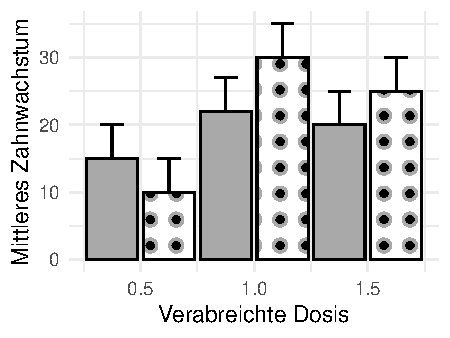
\includegraphics[width=\maxwidth]{img/mc-anova-02-a-1} 

}







\begin{enumerate}
\item [\textbf{A} \msquare] Das Bestimmtheitsmaß $R^2$ ist groß.
\item [\textbf{B} \msquare] Keine Interaktion liegt vor $(p \leq 0.05)$.
\item [\textbf{C} \msquare] Eine mittlere bis starke Interaktion liegt vor $(p \leq 0.05)$
\item [\textbf{D} \msquare] Eine negative Interaktion liegt vor $(\rho \geq 0.5)$.
\item [\textbf{E} \msquare] Die Koeffizienten sind negativ $(\beta_0 < 0; \beta_1 < 0)$.
\end{enumerate} 
\section*{Deskriptive Statistik \& Explorative Datenanalyse}

\section{Aufgabe \hfill (2 Punkte)}




Berechnen Sie den Mittelwert und Standardabweichung von $y$ mit 7, 7, 18, 7 und 9.



\begin{enumerate}
\item [\textbf{A} \msquare] Sie erhalten 9.6 +/- 2.385
\item [\textbf{B} \msquare] Es berechnet sich 9.6 +/- 4.77
\item [\textbf{C} \msquare] Sie erhalten 9.6 +/- 2.18
\item [\textbf{D} \msquare] Es berechnet sich 9.6 +/- 22.8
\item [\textbf{E} \msquare] Es ergibt sich 8.6 +/- 11.4
\end{enumerate} 

\section{Aufgabe \hfill (2 Punkte)}




Wie lautet der Median, das $1^{st}$ Quartile sowie das $3^{rd}$ Quartile von $y$ mit 31, 24, 36, 14, 31, 17, 15, 23, 33, 14 und 51.




\begin{enumerate}
\item [\textbf{A} \msquare] Es ergibt sich 24 +/- 15
\item [\textbf{B} \msquare] Sie erhalten 24 [13; 31]
\item [\textbf{C} \msquare] Es berechnet sich 25 [16; 32]
\item [\textbf{D} \msquare] Sie erhalten 24 +/- 33
\item [\textbf{E} \msquare] Sie erhalten 24 [15; 33]
\end{enumerate} 

\section{Aufgabe \hfill (2 Punkte)}



Sie überlegen Ihre Daten mit einem Dotplot zu visualisieren. Was ist die minimale Anzahl an Beobachtungen pro Gruppe ?



\begin{enumerate}
\item [\textbf{A} \msquare] 10 Beobachtungen.
\item [\textbf{B} \msquare] Die Mindestanzahl liegt bei fünf Beobachtungen.
\item [\textbf{C} \msquare] Dotplot
\item [\textbf{D} \msquare] Die untere Grenze liegt bei einer Beobachtung.
\item [\textbf{E} \msquare] Wir sollten eine Beobachtung mindestens pro Gruppe vorliegen haben.
\end{enumerate}

\section{Aufgabe \hfill (2 Punkte)}



Die Standardabweichung ist eine bedeutende deskriptive Statistik für die Analyse von Daten. Wie müssen Sie vorgehen um die Standardabweichung zu berechnen?



\begin{enumerate}
\item [\textbf{A} \msquare] Als erstes berechnen wir den Mittelwert. Dann bilden wir die Summe der quadratischen Abstände zu dem Mittelwert. Abschließend subtrahieren wir die Fallzahl.
\item [\textbf{B} \msquare] Wir berechnen erst den Mittelwert und dann die absoluten Abstände zu dem Mittelwert. Diese quadratischen Abstände summieren wir auf und teilen am Ende durch die Fallzahl.
\item [\textbf{C} \msquare] Den Mittelwert berechen, dann die absoluten Abstände zum Mittelwert aufsummieren
\item [\textbf{D} \msquare] Den Mittelwert berechen, dann die quadratischen Abstände zum Mittelwert aufsummieren und durch die Fallzahl teilen.
\item [\textbf{E} \msquare] Wir berechnen erst den Mittelwert und dann die quadratischen Abstände zu dem Mittelwert. Diese quadratischen Abstände summieren wir auf und teilen am Ende durch die Fallzahl. Als letzten Schritt ziehen wir die quadratische Wurzel.
\end{enumerate} 

\section{Aufgabe \hfill (2 Punkte)}



Der Barplot stellt folgende statistische Maßzahlen in einer Abbildung dar. Damit gehört der Barplot zu einem der am meisten genutzten statistischen Verfahren zur Visualisierung von Daten.

 



\begin{enumerate}
\item [\textbf{A} \msquare] Der Barplot stellt die Mittelwerte und die Standardabweichung dar.
\item [\textbf{B} \msquare] Den Median und die Standardabweichung.
\item [\textbf{C} \msquare] Der Barplot stellt den Median und die Streuung dar.
\item [\textbf{D} \msquare] Den Median und die Quartile.
\item [\textbf{E} \msquare] Durch die Abbildung des Barplot erhalten wir die Informationen über die Mittelwerte und die Varianz.
\end{enumerate}

\section{Aufgabe \hfill (2 Punkte)}



Nachdem Sie in einem Feldexperiment zu Leistungssteigerung von Maiss durchgeführt haben, berechnen Sie den Mittelwert und den Median. Der Mittelwert $\bar{y}$ und der Median $\tilde{y}$ unterscheiden sich nicht. Welche Aussage ist richtig?



\begin{enumerate}
\item [\textbf{A} \msquare] Da sich der Mittelwert und der Median unterscheiden, ist der Datensatz nicht zu verwenden. Mittelwert und Median müssen gleich sein.
\item [\textbf{B} \msquare] Wenn sich der Mittelwert und der Median nicht unterscheiden, liegen vermutlich Outlier in den Daten vor.
\item [\textbf{C} \msquare] Da sich der Mittelwert und der Median unterscheiden, liegen vermutlich Outlier in den Daten vor. Wir untersuchen den Datensatz nach auffälligen Beobachtungen.
\item [\textbf{D} \msquare] Der Mittelwert und der Median sollten sich unterscheiden sein, wenn Outlier in den Daten vorliegen. 
\item [\textbf{E} \msquare] Da sich der Mittelwert und der Median nicht unterscheiden, liegen vermutlich Outlier in den Daten vor. Wir untersuchen den Datensatz nach auffälligen Beobachtungen.
\end{enumerate}

\section{Aufgabe \hfill (2 Punkte)}



Um zu Überprüfen, ob die Daten die Annahme einer Varianzhomogenität genügen, können wir folgende Visualisierung nutzen. Dabei kommt dann auch die entsprechende Regel zur Abschätzung der Annahme einer Varianzhomogenität zur Anwendung.



\begin{enumerate}
\item [\textbf{A} \msquare] In einer explorativen Datanalyse nutzen wir den Boxplot. Dabei sollte der Median als dicke Linie in der Mitte der Box liegen. Dann können wir von einer Varianzhomogenität ausgehen.
\item [\textbf{B} \msquare] Einen Violinplot. Der Bauch der Violine muss hierbei einen höhren Wert annehmen als der Steg der Violine. Dann kann die Annahme einer Varianzhomogenität angenommen werden.
\item [\textbf{C} \msquare] Einen Dotplot. Die Punkte müssen sich wie an einer Perlenschnurr audreihen. Eine Abweichung führt zur Ablehnung der Annahme einer Varianzhomogenität.
\item [\textbf{D} \msquare] Einen Boxplot. Das IQR muss über alle Behandlungen zusammen mit den Whiskers ungefähr gleich aussehen.
\item [\textbf{E} \msquare] In einer explorativen Datanalyse nutzen wir den Violinplot. Dabei sollte der Bauch am Rand liegen. Dann können wir von einer Varianzhomogenität ausgehen.
\end{enumerate}

\section{Aufgabe \hfill (2 Punkte)}




In der Statistik müssen wir häufig überprüfen, ob unser Outcome einer bestimmten Verteilung folgt. Meistens überprüfen wir, ob eine
Normalverteilung vorliegt. Folgende drei Abbildungen eigenen sich im Besonderen für die Überprüfung einer Verteilungsannahme an eine Variable.





\begin{enumerate}
\item [\textbf{A} \msquare] Barplot, Mosaicplot, Violinplot
\item [\textbf{B} \msquare] Histogramm, Scatterplot, Boxplot
\item [\textbf{C} \msquare] Scatterplot, Mosaicplot, Boxplot
\item [\textbf{D} \msquare] Boxplot, Violinplot, Mosaicplot
\item [\textbf{E} \msquare] Densityplot, Boxplot, Violinplot
\end{enumerate} 

\section{Aufgabe \hfill (2 Punkte)}



Bevor Sie in Ihrer Abschlussarbeit einen statistischen Test rechnen, wollen Sie einmal betrachten, welcher Verteilung Ihre $n = 194$ geernteten Pflanzen folgen.  Welche Verteilung ist abgebildet?



{\centering 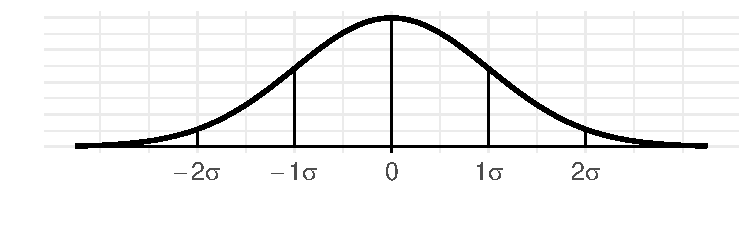
\includegraphics[width=\maxwidth]{img/mc-distribution-02-a-1} 

}







\begin{enumerate}
\item [\textbf{A} \msquare] Es handelt sich um eine Binomial-Verteilung.
\item [\textbf{B} \msquare] In dem Histogramm ist eine Normalverteilung dargestellt.
\item [\textbf{C} \msquare] Dem Histogramm entnehmen wir eine Possion-Verteilung.
\item [\textbf{D} \msquare] Wir haben eine Gammaverteilung vorliegen.
\item [\textbf{E} \msquare] In dem Histogramm ist eine Ordinalverteilung dargestellt.
\end{enumerate} 
\section*{Lineare Regression \& Korrelation}

\section{Aufgabe \hfill (2 Punkte)}



Sie haben das Modell $Y \sim X$ vorliegen und wollen nun ein kausales Modell rechnen. Welche Aussage ist richtig?



\begin{enumerate}
\item [\textbf{A} \msquare] Ein kausales Modell basiert auf einem Traingsdatensatz und einem Testdatensatz. Auf dem Trainingsdatensatz wird das Modell trainiert und auf dem Testdatensatz validiert.
\item [\textbf{B} \msquare] Ein kausales Modell möchte die Zusammenhänge von X auf Y modellieren. Hierbei geht es um die Effekte von $X$ auf $Y$. Man sagt, wenn $x_1$ um 1 ansteigt ändert sich $Y$ um einen Betrag $\beta_1$.
\item [\textbf{C} \msquare] Wenn ein kausales Modell gerechnet werden soll dann kann dies auf dem gesamten Datensatz geschehen. Das Ziel ist es einen Zusammenhang von $X$ auf $Y$ zu modellieren. Wie wirken sich die Einflussvariablen $Y$ auf die gemessenen Endpunkte $X = x_1, ..., x_p$ aus?
\item [\textbf{D} \msquare] Ein kausales Modell benötigt mindestens eine Fallzahl von über 100 Beobachtungen und darf keine fehlenden Werte beinhalten. Die Varianzkomponenten müssen homogen sein.
\item [\textbf{E} \msquare] Ein kausales Modell wird auf einem Trainingsdatensatz trainiert und anschliessend über eine explorative Datenanalyse validiert. Signifikanzen über $\beta_i$ können hier nicht festgestellt werden.
\end{enumerate}

\section{Aufgabe \hfill (2 Punkte)}



Nach einer Regressions sollten die Residuen normalverteilt sein. Was bei einer simplen Regression noch relativ einfach visuell in einem Scatterplot zu überprüfen ist. Für komplexere Modell liefert der QQ-Plot die notwendigen Informationen über die Normalverteilung. Welche Aussage ist richtig?



{\centering 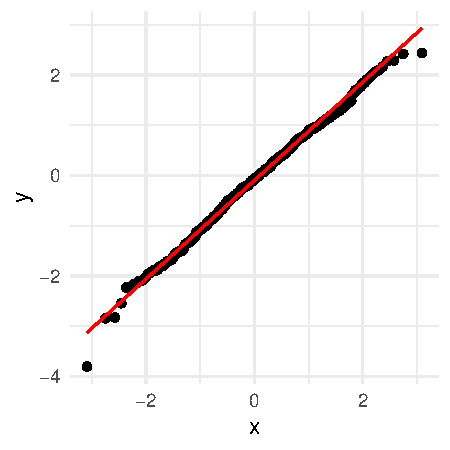
\includegraphics[width=\maxwidth]{img/mc-regression-05-a-1} 

}







\begin{enumerate}
\item [\textbf{A} \msquare] Wir betrachten die Gerade, die durch die einzelnen Punkte laufen sollte. Wenn die 95\% der Punkte von der Geraden getroffen werden, dann gehen wir von normalverteilten Residuen aus.
\item [\textbf{B} \msquare] Wir betrachten insbesondere die beiden Enden der Gerade. Der Rest ist mehr oder minder egal, dann ist die Annahme an die Normalverteilung der Residuen erfüllt.
\item [\textbf{C} \msquare] Die Annahme der normalverteilten Residuen ist erfüllt. Die Punkte liegen zum überwiegenden Teil nicht auf der Geraden.
\item [\textbf{D} \msquare] Wir betrachten die Gerade und dabei insbesondere die beiden Enden der Gerade. Hier sollten die Punkte auf der Geraden liegen, dann ist die Annahme an die Normalverteilung der Residuen erfüllt.
\item [\textbf{E} \msquare] Wir betrachten die Gerade und dabei insbesondere die beiden Enden der Gerade in dem IQR, also dem ersten und dritten Quartile. Hier sollten die Punkte auf der Geraden liegen, dann ist die Annahme an die Normalverteilung der Residuen erfüllt.
\end{enumerate}

\section{Aufgabe \hfill (2 Punkte)}



Sie rechnen eine linearen Regression und erhalten folgende Abbildung der Residuen (\texttt{.resid}). Welche Aussage ist richtig?



{\centering 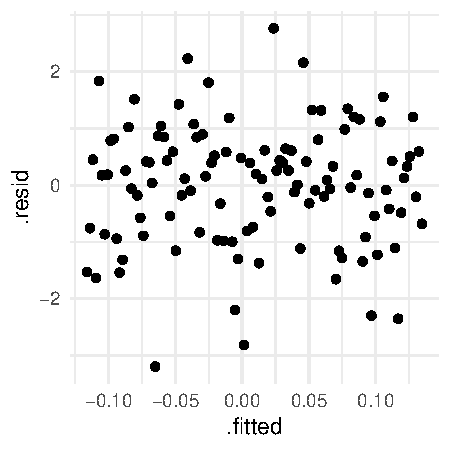
\includegraphics[width=\maxwidth]{img/mc-regression-06-a-1} 

}







\begin{enumerate}
\item [\textbf{A} \msquare] Wenn die Punkte gleichmäßig in dem positiven wie auch negativen Bereich ohne ein klares Muster liegen, dann hat unsere Modellierung geklappt. Wir können mit dem Modell weitermachen.
\item [\textbf{B} \msquare] Wenn wir die Nulllinie betrachten so müssen die Punkte gleichmäßig unter der Nulllinie liegen. Unser Modell erfüllt somit nicht die Annahme von normalverteilten Residuen mit einem Mittelwert von $>0$ und einer Streuung von $s$.
\item [\textbf{C} \msquare] Die Punkte müssen gleichmäßig, mit ähnlichen Abständen, in dem positiven wie auch negativen Bereich liegen. Dies ist hier klar nicht der Fall. Einzelne Ausreißer können beobachtet werden. Wir können mit dem Model so nicht rechnen und müssen erst die auffälligen Werte gesondert betrachten.
\item [\textbf{D} \msquare] Die Annahme der normalverteilten Residuen ist nicht erfüllt. Es ist kein Muster zu erkennen.
\item [\textbf{E} \msquare] Die Annahme der normalverteilten Residuen ist erfüllt. Es ist ein Muster zu erkennen und wir können damit auf die Signifkanz von $x_1, ..., x_p$ schließen.
\end{enumerate}

\section{Aufgabe \hfill (2 Punkte)}




In den Humanwissenschaften wird der Korrelationskoeffizienten $\rho$ sehr häufig verwendet. Daher ist es auch wichtig für andere Forschende den Korrelationskoeffizienten $\rho$ zu verstehen. Welche Aussazu zu dem Korrelationskoeffizienten $\rho$ ist richtig?




\begin{enumerate}
\item [\textbf{A} \msquare] Der Korrelationskoeffizienten $\rho$ liegt zwischen -1 und 1. Darüber hinaus ist der Korrelationskoeffizienten $\rho$ als standardisierte Steigung zu verstehen, wenn eine Standardisierung durchgeführt wurde. Diese Adjustierung nach Fischer muss am Anschluß der Berechnung der Korrelation durchgeführt werden.
\item [\textbf{B} \msquare] Der Korrelationskoeffizienten $\rho$ zeigt keinen Zusammenhang zwischen zwei Variablen $x$ und $y$ bei einem Wert von 0. Einen maximalen negativen Zusammenhang bei -1 und somit auch einen maximalen positiven Zusammenhang bei 1. Korrelationskoeffizienten $\rho$ ist einheitslos.
\item [\textbf{C} \msquare] Der Korrelationskoeffizienten $\rho$ ist eine standardisierte, statistische Maßzahl, die zwischen 0 und 1 liegt. Dabei ist Korrelationskoeffizienten $\rho$ einheitslos. Eine Signifikanz kann nicht nachgewiesen werden.
\item [\textbf{D} \msquare] Korrelationskoeffizienten $\rho$ liegt zwischen 0 und 1. Darüber hinaus ist der Korrelationskoeffizienten $\rho$ einheitslos und kann als Standardisierung verstanden werden.
\item [\textbf{E} \msquare] Der Korrelationskoeffizienten $\rho$ wird wie das $\eta^2$ aus der ANOVA interpretiert. Der Korrelationskoeffizienten $\rho$ beschreibt den Anteil an erklärter Varianz durch die Regression. Dabei gibt er jedoch eine Richtung an und kann auch negativ werden.
\end{enumerate}

\section{Aufgabe \hfill (2 Punkte)}



Sie haben ein Feldexperiment mit Brokkoli durchgeführt und wollen nun in einer simplen linearen Regression den Einfluss der $CO_2$-Konzentration in [$\mu g$] im Wasser auf das Trockengewicht in [$kg$] untersuchen. Sie erhalten einen $\beta_{CO_2}$ Koeffizienten von $1.1\times 10^{-5}$ und einen $p$-Wert mit $1e-04$. Welche Aussage zu der Signifikanz und dem Effekt ist richtig?




\begin{enumerate}
\item [\textbf{A} \msquare] Wenn der Effekt $\beta_{CO_2}$ winzig ist, dann kann es an einer falsch gewählten Einheit liegen. Der Anstieg von einer Einheit in $X$ führt ja zu einer Änderung von $\beta_{CO_2}$ in $x$. Wir müssen daher die Einheit von $y$ entsprechend anpassen.
\item [\textbf{B} \msquare] Manchmal ist die Einheit der Einflussvariable $X$ zu groß gewählt, so dass der Ansteig von 1 Einheit in $X$ zu einer zu großen Änderung in $y$ führt. Daher kann der Effekt $\beta_{CO_2}$ sehr klein wirken, da der p-Wert wird auf einer einheitslosen Teststatistik bestimmt wird.
\item [\textbf{C} \msquare] Die Fallzahl ist zu klein angesetzt. Je kleiner die Fallzahl ist, desto höher ist die Teststatsitik und damit auch der $p$-Wert kleiner. Wir brauchen also mehr Fallzahl um den geringen Effekt noch signifikant zu krigen.
\item [\textbf{D} \msquare] Manchmal ist die Einheit der Einflussvariable $X$ zu klein gewählt, so dass der Ansteig von 1 Einheit in $X$ zu einer zu kleinen Änderung in $y$ führt. Daher kann der Effekt $\beta_{CO_2}$ sehr klein wirken, aber auf einer anderen Einheit sehr viel größer sein. Der p-Wert wird auf einer einheitslosen Teststatistik bestimmt.
\item [\textbf{E} \msquare] Die Einheit der $CO_2$-Konzentration ist zu klein gewählt. Dadurch sehen wir den sehr kleinen $p$-Wert. Der $p$-Wert und die Einheit von der $CO_2$-Konzentration hängen antiproportional zusammen.
\end{enumerate}

\section{Aufgabe \hfill (2 Punkte)}



Sie wollen nach der explorativen Datenanalyse (EDA) Ihre Daten in der Abschlussarbeit auswerten. Nach einiger Rechereche finden Sie heraus, dass Sie zuerst die Daten mit der Funktion \texttt{lm()} in \Rlogo modellieren müssen. Welche Anwendung folgt drauf?





\begin{enumerate}
\item [\textbf{A} \msquare] Neben der klassichen Verwendung der Funktion \texttt{lm()} in der linearen Regression kann auch ein Gruppenvergleich gerechnet werden. Dafür müssen aber alle Faktoren aus den Daten entfernt und numerishc umgewandelt werden. Dann kann das R Paket \{emmeans\} genutzt werden um die Korrelation zu berechnen. Eine Adjustierung ist dann nicht mehr notwendig.
\item [\textbf{B} \msquare] Die Funktion \texttt{lm()} in \Rlogo wird klassischerweise für die lineare Regression genutzt. Ist die Einflussvariable $X$ ein Faktor so werden die Gruppenmittelwerte geschätzt und eine anschließende ANOVA sowie multipler Gruppenvergleich mit \{emmeans\} ist möglich.
\item [\textbf{C} \msquare] Die Funktion \texttt{lm()} in \Rlogo wird klassischerweise für die nicht-lineare Regression genutzt. Ist die Einflussvariable $X$ numerisch so werden die Gruppenmittelwerte geschätzt.
\item [\textbf{D} \msquare] Ist die Einflussvariable $X$ ein Faktor so werden die Gruppenmittelwerte geschätzt und eine anschließende ANOVA sowie multipler Gruppenvergleich mit \{emmeans\} ist möglich. Die Funktion \texttt{lm()} kann dabei eigentlich weggelassen werden, wird aber traditionell gerechnet.
\item [\textbf{E} \msquare] Ist die Einflussvariable $X$ numerisch so werden die Gruppenmittelwerte geschätzt und eine anschließende ANOVA sowie multipler Gruppenvergleich mit \{emmeans\} ist möglich.
\end{enumerate}

\section{Aufgabe \hfill (2 Punkte)}



In Ihrer Abschlussarbeit haben Sie neben den klassischen normalverteilten Endpunkte, wie Trockgewicht und Wuchshöhe noch den Infektionsstatus und Zähldaten erhoben. Um diese nicht normalverteilten Endpunkte auszuwerten nutzen Sie das \textit{generalisierte lineare Modell (GLM)}. Welche Aussage ist richtig?




\begin{enumerate}
\item [\textbf{A} \msquare] Das GLM ist eine Vereinfachung des LM in R. Mit dem GLM lassen sich polygonale Regressionen rechnen. Somit stehen neben der Normalverteilung noch weitere Verteilungen zu Verfügung.
\item [\textbf{B} \msquare] Das GLM erlaubt auch nicht normalverteilte Residuen in der Schätzung der Regressionsgrade.
\item [\textbf{C} \msquare] Das \textit{generalisierte lineare Modell (GLM)} erlaubt auch weitere Verteilungsgruppen für das $X$ bzw. die Einflussvariablen in einer linearen Regression zu wählen.
\item [\textbf{D} \msquare] Dank dem \textit{generalisierten linearen Modell (GLM)} können auch andere Verteilungsfamilien als die Normalverteilung mit einer linearen Regression modelliert werden.
\item [\textbf{E} \msquare] In \Rlogo ist mit dem \textit{generalisierten linearen Modell (GLM)} eine Modellierung implementiert, die die Poissonverteilung für Zähldaten oder die Binomialverteilung für 0/1-Daten modellieren kann. Weitere Modellierungen sind in \Rlogo auch mit zusätzlich geladenen Paketen nicht möglich.
\end{enumerate}
\section*{Vermischte Themen}  

\section{Aufgabe \hfill (2 Punkte)}

Die Randomisierung von Beobachtungen zu den Versuchseinheiten
ist bedeutend in der Versuchsplanung. Welche der folgenden Aussagen ist richtig?



\begin{enumerate}
\item [\textbf{A} \msquare] Durch eine Randomisierung können wir nicht von Strukturgleichheit zwischen der Stichprobe und der Grundgesamtheit ausgehen.
\item [\textbf{B} \msquare] Randomisierung war bis 1952 bedeutend, wurde dann aber in Folge besserer Rechnerleistung nicht mehr verwendet. Aktuelle Statistik nutzt keine Randomisierung mehr.
\item [\textbf{C} \msquare] Randomisierung ist die direkte Folge von Strukturgleichheit. Die Strukturgleichheit erlaubt es erst von der Stichprobe auf die Grundgesamtheit zurückzuschliessen.
\item [\textbf{D} \msquare] Randomisierung sorgt für Strukturgleichheit und erlaubt erst von der Stichprobe auf die Grundgesamtheit zurückzuschliessen.
\item [\textbf{E} \msquare] Strukturgleichheit ist durch Randomisierung gegeben. Leider hilft die Randomisierung noch nicht um von der Stichprobe auf die Grundgesamtheit zu schließen. Deshalb wurde das Falsifikationsprinzip entwickelt.
\end{enumerate}

\section{Aufgabe \hfill (2 Punkte)}



Wenn Sie einen Datensatz erstellen, dann ist es ratsam die Spalten und die Einträge in englischer Sprache zu verfassen, wenn Sie später die Daten in \Rlogo auswerten wollen. Welcher Aussage ist richtig?



\begin{enumerate}
\item [\textbf{A} \msquare] Programmiersprachen können nur englische Begriffe verarbeiten. Zusätzliche Pakete können zwar geladen werden, aber meist funktionieren diese Pakete nicht richtig. Deutsch ist International nicht bedeutend genug.
\item [\textbf{B} \msquare] Die Spracherkennung von \Rlogo ist nicht in der Lage Deutsch zu verstehen.
\item [\textbf{C} \msquare] Die \Rlogo Pakete sind nur in englischer Sprache verfasst. Das ist aber nicht der Hauptgrund, denn \Rlogo hat wie alle Programmiersprachen Probelem mit Umlauten und Sonderzeichen.
\item [\textbf{D} \msquare] Alle Funktionen und auch Anwendungen sind in \Rlogo in englischer Sprache. Die Nutzung von deutschen Wörtern ist nicht schick und das ist zu vermeiden.
\item [\textbf{E} \msquare] Programmiersprachen haben Probleme mit Umlauten und Sonderzeichen der deutschen Sprache. Daher ist die Nutzung in Deutsch in den AGBs von \Rlogo untersagt.
\end{enumerate}

\section{Aufgabe \hfill (2 Punkte)}



In Ihrer Abschlussarbeit wollen Sie zu Beginn eine explorativen Datenanalyse (EDA) in \Rlogo rechnen. Dafür gibt es eine generelle Abfolge von Prozessschritten. Welche ist hierbei die richtige Reihenfolge?



\begin{enumerate}
\item [\textbf{A} \msquare] Wir transformieren die Spalten über \texttt{mutate()} in ein \texttt{tibble} und können dann über \text{ggplot()} uns die Abbildungen erstellen lassen. Dabei beachten wir das wir keine Faktoren in den Daten haben.
\item [\textbf{B} \msquare] Die Funktionsreihenfolge ist wie folgt: \texttt{read\_excel()} ->  \texttt{mutate()} -> \text{ggplot()}. Dabei ist bei der Transformation der Daten darauf zu achten, dass keine Faktoren erstellt werden.
\item [\textbf{C} \msquare] Die Funktionsreihenfolge ist wie folgt: \texttt{read\_excel()} ->  \texttt{mutate()} -> \text{ggplot()}. Dabei ist bei der Transformation der Daten darauf zu achten, dass die Faktoren richtig erstellt werden.
\item [\textbf{D} \msquare] Für eine explorativen Datenanalyse (EDA) in \Rlogo müssen wir als erstes die Daten über \texttt{read\_excel()} einlesen. Danach müssen wir schauen, dass wir die Zeilen richtig über \texttt{mutate()} transformiert haben. Insbesondere müssen Variablen mit kontinuierlichen Werten in einen Faktor umgewandelt werden. Am Ende nutzen wir die Funktion \text{ggplot()} für die eigentlich EDA.
\item [\textbf{E} \msquare] Wir lesen die Daten über eine generische Funktion \texttt{read()} ein und müssen dann die Funktion \texttt{ggplot()} nur noch installieren. Dann haben wir die Abbildungen als \texttt{*.png} vorliegen.
\end{enumerate}

\section{Aufgabe \hfill (2 Punkte)}



Gegeben ist das Modell $Y \sim X$. Welche Aussage über $s^2_1 \neq s^2_2$ ist richtig?



\begin{enumerate}
\item [\textbf{A} \msquare] Es handelt sich um ein balanciertes Design.
\item [\textbf{B} \msquare] Es liegt Varianzhomogenität vor.
\item [\textbf{C} \msquare] Es handelt sich um abhängige Beobachtungen.
\item [\textbf{D} \msquare] Es liegt Varianzhetrogenität vor.
\item [\textbf{E} \msquare] Es handelt sich um ein unbalanciertes Design.
\end{enumerate}

\section{Aufgabe \hfill (2 Punkte)}



Die Leistung von Sauen soll auf einem Zuchtbetrieb gesteigert werden. Dafür werden die Ferkel verschiedener Sauen gemessen. Die Ferkel einer Muttersaue sind daher...



\begin{enumerate}
\item [\textbf{A} \msquare] Die Ferkel stammen von der gleichen Sau und sind somit untereinander abhängig.
\item [\textbf{B} \msquare] Untereinander abhängig, wenn die Mütter ebenfalls miteinander verwandt sind. Erst die Abhängigkeit 2. Grades wird in der Statistik modelliert.
\item [\textbf{C} \msquare] Die Ferkel stammen von der gleichen Sau und sind somit untereinander unabhängig.
\item [\textbf{D} \msquare] Untereinander unabhängig. Sollten die Mütter verwandt sein, so ist die Varianzstruktur ähnlich und muss modelliert werden.
\item [\textbf{E} \msquare] Je nach Stallanlage kommt eine andere Analyse in Betracht. Eine allgemeine Aussage über Ferkel und Sauen lässt sich statistisch nicht treffen.
\end{enumerate}

\section{Aufgabe \hfill (2 Punkte)}



Neben der Mittelwertsdifferenz als Effektschätzer bei normalverteilten Endpunkten wird auch häufig der Effektschätzer Odds ratio bei binären Endpunkten verwendet. Welche Aussage über den Effektschätzer Odds ratio ist im folgenden Beispiel zur Behandlung von Klaueninfektionen bei Rinder richtig? Dabei sind 6 Tiere krank und 7 Tiere sind gesund.



\begin{enumerate}
\item [\textbf{A} \msquare] Da es sich um ein Chancenverhältnis handelt ergibt sich ein Odds ratio von 0.86.
\item [\textbf{B} \msquare] Es ergibt sich ein Odds ratio von 0.46, da es sich um ein Anteil handelt. Wir berechnen den Anteil der Kranken.
\item [\textbf{C} \msquare] Da es sich um ein Chancenverhältnis handelt ergibt sich ein Odds ratio von 2.17.
\item [\textbf{D} \msquare] Es ergibt sich ein Odds ratio von 0.86, da es sich um ein Anteil handelt.
\item [\textbf{E} \msquare] Es ergibt sich ein Odds ratio von 0.46, da es sich um eine Chancenverhältnis handelt.
\end{enumerate}

\section{Aufgabe \hfill (2 Punkte)}



Sie werten in Ihrer Abschlussarbeit einen sehr großen Datensatz aus einer öffentlichen Datenbank aus. Nun stellen Sie fest, dass Sie ein Problem mit der Bewertung Ihrer Ergbnisse anhand der Signifikanz bekommen. Wie Sie herausfinden, scheint dies ein häufiges Problem in der Bio Data Science zu sein. Welche Aussage ist richtig?




\begin{enumerate}
\item [\textbf{A} \msquare] Aktuell werden immer größere Datensätze erhoben. Dadurch wird auch die Varianz immer höher was automatisch zu mehr signifikanten Ergebnissen führt.
\item [\textbf{B} \msquare] Aktuell werden immer größere Datensätze erhoben. Eine erhöhte Fallzahl führt automatisch auch zu mehr signifikanten Ergebnissen, selbst wenn die eigentlichen Effekte nicht relevant sind.
\item [\textbf{C} \msquare] Big Data ist ein Problem der parametrischen Statistik. Parameter lassen sich nur auf kleinen Datensätzen berechnen, da es sich sonst nicht mehr um eine Stichprobe im engen Sinne der Statistik handelt.
\item [\textbf{D} \msquare] Mehr Fallzahl in Datensätzen bedeutet mehr signifikante Ergebnisse, da in mehr Daten auch mehr Informationen beinhaltet sind. Deshalb lohnen sich riesige Datensätze, die durch die vielen signifikanten Ergebnisse auch eine Menge an relevanten Erkenntnissen liefern.
\item [\textbf{E} \msquare] Aktuell werden zu grosse Datensätze für die gänigige Statistik gemessen. Daher wendet man maschinelle Lernverfahren für kausale Modelle an. Hier ist die Relevanz gleich Signifikanz.
\end{enumerate}
\section*{Multiple Gruppenvergleiche}    

\section{Aufgabe \hfill (2 Punkte)}



Sie haben folgende unadjustierten p-Werte gegeben: 0.21, 0.34, 0.001 und 0.01. Sie adjustieren die p-Werte nach
Bonferroni. Welche Aussage ist richtig?



\begin{enumerate}
\item [\textbf{A} \msquare] Nach der Bonferroni-Adjustierung ergeben sich die adjustierten p-Werte von 0.84, 1, 0.004 und 0.04. Die adjustierten p-Werte werden zu einem $\alpha$-Niveau von 1.25\% verglichen.
\item [\textbf{B} \msquare] Nach der Bonferroni-Adjustierung ergeben sich die adjustierten p-Werte von 0.84, 1, 0.004 und 0.04. Die adjustierten p-Werte werden zu einem $\alpha$-Niveau von 5\% verglichen.
\item [\textbf{C} \msquare] Nach der Bonferroni-Adjustierung ergeben sich die adjustierten p-Werte von 0.84, 1.36, 0.004 und 0.04. Die adjustierten p-Werte werden zu einem $\alpha$-Niveau von 5\% verglichen.
\item [\textbf{D} \msquare] Nach der Bonferroni-Adjustierung ergeben sich die adjustierten p-Werte von 0.0525, 0.085, 3e-04 und 0.0025. Die adjustierten p-Werte werden zu einem $\alpha$-Niveau von 1.25\% verglichen.
\item [\textbf{E} \msquare] Nach der Bonferroni-Adjustierung ergeben sich die adjustierten p-Werte von 0.0525, 0.085, 3e-04 und 0.0025. Die adjustierten p-Werte werden zu einem $\alpha$-Niveau von 5\% verglichen.
\end{enumerate}

\section{Aufgabe \hfill (2 Punkte)}



Auf wissenschaftlichen Postern finden Sie unter Abbildungen häufig die Abbkürzung \textit{CLD}. Für welchen statistischen Fachbegriff steht die Abbkürzung und wie interpretieren Sie ein \textit{CLD}?



\begin{enumerate}
\item [\textbf{A} \msquare] Compact letter display. Das CLD ist umstritten, da es die Gleichheit der Behandlungen durch gleiche Buchstaben darstellt. Dadurch ist das CLD nicht mehr sauber auf einer Linie mit dem statistischen Testen. Wir lehnen die Nullhypothese ab und zeigen keine Gleichheit im statistischen Testen.
\item [\textbf{B} \msquare] Compact letter detection. Gleichheit in den Behandlungen wird durch den gleichen Buchstaben oder Symbol dargestellt.
\item [\textbf{C} \msquare] Compact letter display. Gleiche Buchstaben zeigen Gleichheit in den Behandlungen. Die Interpretation ist deshalb sehr intuitiv und einfach. Darüber hinaus ist damit das CLD auch auf einer Linie mit der Testtheorie, da wir ja auch dort die Gültigkeit der Nullhypothese nachweisen. Wir suchen ja Gleichheit.
\item [\textbf{D} \msquare] Compact line display. Gleichheit in den Behandlungen wird durch den gleichen Buchstaben oder Symbol dargestellt. Früher wurden keine Buchstaben sondern eine durchgezogene Linie verwendet. Bei mehr als drei Gruppen funktioniert die Linie aber graphisch nicht mehr.
\item [\textbf{E} \msquare] Compact letter display. Gleiche Buchstaben bedeuten, dass sich die Behandlungen unterscheiden. Daher ist das CLD sehr unintuitiv. Es wäre besser, wenn gleiche Buchstaben Gleichheit anzeigen würden. Dies ist aber leider in der statistischen Testtheorie nicht möglich.
\end{enumerate}

\section{Aufgabe \hfill (2 Punkte)}




Der multiple Vergleich als Posthoc-Test nach einer ANOVA ist in den Agrarwissenschaften heutzutage Standard. Welches R Paket wird häufig für den multiplen Vergleich genutzt? Welche Beschreibung der Eigenschaften ist korrekt?



\begin{enumerate}
\item [\textbf{A} \msquare] Das R Paket \{hmisc\} erlaubt die Durchführung eines multiplen Gruppenvergleichs aus verschiedenen Modellen heraus. Aus einem hmisc Objekt lässt sich recht einfach das CLD erstellen und so über Barplots eine schnelle Interpration der statistischen Auswertung durchführen.
\item [\textbf{B} \msquare] Das R Paket \{ggplot\}. Wir erhalten hier sofort eine Visualisierung der Daten. Anhand der Visualisierung lässt sich eine explorative Datenanalyse durchführen, die gleichwertig zu einem Posthoc-Test ist.
\item [\textbf{C} \msquare] Da Sie für Ihre Bachelorarbeit einen Barplot mit CLD brauchen nutzen Sie das R Paket \{emmeans\} welches Ihnen schnell die notwenidigen Informationen liefert um einen Barplot zu erstelen. Die Berechnung eines CLD ist hierbei auch einfach.
\item [\textbf{D} \msquare] Das R Paket \{lm\}. Das Paket \{lm\} erstellt selbstständig Konfidenzintervalle und entsprechende p-Werte. Da wir in dem Paket nicht adjustieren müssen, ist es bei Anwendern sehr beliebt.
\item [\textbf{E} \msquare] Das R Paket \{emmeans\} erlaubt die Durchführung eines multiplen Gruppenvergleichs. Aus einem emmeans Objekt lässt sich leider kein CLD erstellen. Dennoch ist das Paket einfach zu bedienen und wird deshalb genutzt. Die Interpretation der statistischen Auswertung wird über einen Barplot abgebildet.
\end{enumerate}

\section{Aufgabe \hfill (2 Punkte)}



Bei einem Posthoc-Test kann es zu einer überraschenden Besonderheit beim statistischen Testen kommen. Wie lautet der Fachbegriff und wie kann mit der überraschenden Besonderheit umgegangen werden?



\begin{enumerate}
\item [\textbf{A} \msquare] Die Adjustierung der p-Werte nach Bonferroni erlaubt es gegen die $\alpha$-Inflation vorzugehen, die häufig beim multiplen Testen auftritt. Das globale Signifikanzniveau liegt nicht mehr bei $5\%$ sondern sehr viel höher. Das ist der Grund warum die p-Werte entsprechend adjustiert werden müssen.
\item [\textbf{B} \msquare] Die Adjustierung der p-Werte nach Bonferroni erlaubt es gegen die $\beta$-Inflation vorzugehen, die häufig beim multiplen Testen auftritt. Das globale Powerniveau liegt nicht mehr bei $80\%$ sondern sehr viel niedriger.
\item [\textbf{C} \msquare] Beim multiplen Testen kann es zu einer $\alpha$-Deflation kommen. Das globale Signifikanzniveau liegt nicht mehr bei $5\%$ sondern weit darunter. Daher müssen die p-Werte entsprechend adjustiert werden. Hierfür gibt es verschiedene Verfahren, wobei das Verfahren zur Adjustierung der p-Werte nach Bonferroni das bekanneste Verfahren ist. Die p-Werte werden durch die Anzahl an Vergleichen geteilt
\item [\textbf{D} \msquare] Das globale Signifikanzniveau explodiert und erreicht Werte größer als Eins. Es kommt zu einer $\alpha$-Inflation. Dagegen kann mit der Adjustierung der $\alpha$-Werte nach Bonferroni vorgegangen werden.
\item [\textbf{E} \msquare] Das globale Signifikanzniveau liegt nicht mehr bei $5\%$ sondern sehr viel niedriger, bei ca. $1\%$. Es kommt zu einer $\alpha$-Hyperinflation. Dagegen kann mit der Adjustierung der p-Werte nach Bonferroni vorgegangen werden.
\end{enumerate}

\section{Aufgabe \hfill (2 Punkte)}




In einem Feldversuch haben Sie einen Behandlungsfaktor mit mehreren Leveln vorliegen. Sie rechnen einen multiplen Vergleich. Vorher hatten Sie eine einfaktorielle ANOVA mit einem signifikanten Ergebnis vorliegen. Welche Aussage ist richtig?



\begin{enumerate}
\item [\textbf{A} \msquare] Wenn ein multipler Test gerechnet wird, dann muss der Effekt $\Delta$ adjustiert werden im Gegensatz zu den p-Werten.
\item [\textbf{B} \msquare] Beim multiplen Testen kann es zu einer $\Delta$-Deflation kommen. Das globale Relevanzniveau liegt nicht mehr bei $5\%$ sondern weit darunter. Daher müssen die $\Delta$-Werte entsprechend adjustiert werden. Hierfür gibt es verschiedene Verfahren, wobei das Verfahren zur Adjustierung der $\Delta$-Werte nach Bonferroni das bekanneste Verfahren ist. Die $\Delta$-Werte werden durch die Anzahl an Vergleichen geteilt.
\item [\textbf{C} \msquare] Beim multiplen Testen muss der Effekt, hier der Mittelwertsunterschied $\Delta$ aus den paarweisen t-Tests, nicht adjusiert werden.
\item [\textbf{D} \msquare] Beim multiplen Testen kann es zu einer $\Delta$-Inflation kommen. Das globale Effektniveau liegt nicht mehr bei $20\%$. Daher müssen die Effekte entsprechend adjustiert werden. Hierfür gibt es verschiedene Verfahren, wobei das Verfahren zur Adjustierung der Effekte nach Bonferroni das bekanneste Verfahren ist.
\item [\textbf{E} \msquare] Beim multiplen Testen werden die Effekte der paarweisen Vergleiche ignoriert. Der Nachteil des multiplen Testens ist ja auch, dass wir am Ende keine Effekte mehr vorliegen haben. Eine ANOVA liefert hier bessere Informationen.
\end{enumerate}
\section*{Statistische Testtheorie}  

\section{Aufgabe \hfill (2 Punkte)}




Welche Aussage zum mathematische Ausdruck $Pr(D|H_0)$ ist richtig?



\begin{enumerate}
\item [\textbf{A} \msquare] $Pr(D|H_0)$ ist die Wahrscheinlichkeit nicht die Daten $D$ zu beobachten sondern die Nullhypothese, wenn diese wahr ist.
\item [\textbf{B} \msquare] $Pr(D|H_0)$ ist die Wahrscheinlichkeit die Daten $D$ zu beobachten, wenn die Nullhypothese wahr ist.
\item [\textbf{C} \msquare] Die Inverse der Wahrscheinlichkeit unter der die Nullhypothese nicht mehr die Alternativehypothese überdeckt.
\item [\textbf{D} \msquare] Die Wahrscheinlichkeit der Daten unter der Nullhypothese in der Grundgesamtheit.
\item [\textbf{E} \msquare] $Pr(D|H_0)$ stellt die Wahrscheinlichkeit die Teststatistik $T$ zu beobachten dar, wenn die Nullhypothese falsch ist.
\end{enumerate}

\section{Aufgabe \hfill (2 Punkte)}



Das statistische Testen basiert auf dem Falsifikationsprinzip. Es besagt,



\begin{enumerate}
\item [\textbf{A} \msquare] ... dass in der Wissenschaft immer etwas falsch sein muss. Sonst gebe es keinen Fortschritt.
\item [\textbf{B} \msquare] ... dass ein minderwertes Modell durch ein weniger minderwertiges Modell ersetzt wird. Es gilt das Falsifikationsprinzip nach Karl Popper.
\item [\textbf{C} \msquare] ... dass Fehlerterme in statistischen Modellen nicht verifiziert werden können.
\item [\textbf{D} \msquare] ... dass Annahmen an statistische Modelle meist falsch sind.
\item [\textbf{E} \msquare] ... dass Modelle meist falsch sind und selten richtig.
\end{enumerate}

\section{Aufgabe \hfill (2 Punkte)}



Das Signifikanzniveau $\alpha$ wird auch Fehler 1. Art genannt und liegt bei 5\%. Warum wurde der Grenzwert von 5\% als Signifikanzschwelle gewählt?



\begin{enumerate}
\item [\textbf{A} \msquare] Als Kulturkonstante hat $\alpha = 5\%$ den Rang einer Naturkonstante und wurde nach langer Diskussion in der UN im Jahre 1983 festgesetzt. Damals auch schon mit der Zustimmung der UdSSR.
\item [\textbf{B} \msquare] Der Wert ergab sich aus einer Auswertung von 1042 wissenschaftlichen Veröffentlichungen zwischen 1914 und 1948. Der Wert $5\%$ wurde in $28\%$ der Veröffentlichungen genutzt. Daher legte man sich auf diese Zahl fest.
\item [\textbf{C} \msquare] In der Wissenschaft gibt es neben der Naturkonstante, die sich aus der Beobachtung der Welt ergibt, noch die Kulturkonstante, die von einer Gruppe Menschen selbstgewählt wird. Dabei ist $\alpha = 5\%$ eine Kulturkonstante und wurde somit eher zufällig gewählt.
\item [\textbf{D} \msquare] Der Begründer der modernen Statistik, R. Fischer, hat die Grenze simuliert und berechnet. Dadurch ergibt sich dieser optimale Cut-Off.
\item [\textbf{E} \msquare] Im Rahmen eines langen Disputs zwischen Neyman und Fischer wurde $\alpha = 5\%$ festgelegt. Leider werden die Randbedingungen und Voraussetzungen an statistsiche Modelle heute immer wieder ignoriert.
\end{enumerate}

\section{Aufgabe \hfill (2 Punkte)}

Betrachten wir die Teststatistik aus einem abstrakteren Blickwinkel. Beim
statistischen Testen wird das \textit{"`signal"'} mit dem
\textit{"`noise"'} aus den Daten $D$ zu einer Teststatistik $T_D$ verrechnet. Welche der Formel
berechnet korrekt die Teststatistik $T_D$?



\begin{enumerate}
\item [\textbf{A} \msquare] Es gilt $T_D = (signal \cdot noise)^2$
\item [\textbf{B} \msquare] Es gilt $T_D = \cfrac{signal}{noise}$
\item [\textbf{C} \msquare] Es gilt $T_D = signal \cdot noise$
\item [\textbf{D} \msquare] Es gilt $T_D = \cfrac{signal}{noise^2}$
\item [\textbf{E} \msquare] Es gilt $T_D = \cfrac{noise}{signal}$
\end{enumerate}

%% ------------------------------------------------------------

\section{Aufgabe \hfill (2 Punkte)}



Sie versuchen folgende Aussage richtig in die Analogie der statistischen Testtheorie zu setzen. Welche Analogie ist richtig?

\begin{center}
\textit{$H_0$ beibehalten obwohl die $H_0$ falsch ist}
\end{center}



\begin{enumerate}
\item [\textbf{A} \msquare] In die Analogie eines brennenden Hauses ohne Rauchmelder: \textit{House without noise}.
\item [\textbf{B} \msquare] In die Analogie eines Rauchmelders: \textit{Alarm without fire}, dem $\alpha$-Fehler.
\item [\textbf{C} \msquare] In die Analogie eines Rauchmelders: \textit{Alarm without fire police}, dem $\alpha$-Fehler.
\item [\textbf{D} \msquare] \textit{Fire without alarm}, dem $\beta$-Fehler als Analogie von Rauch im Haus.
\item [\textbf{E} \msquare] Dem $\beta$-Fehler mit der Analogie eines Rauchmelders: \textit{Fire without alarm}.
\end{enumerate}

\section{Aufgabe \hfill (2 Punkte)}



Sie lesen eine wissenschaftliche Arbeit, die damit wirbt, dass Effekte und Signifikanz nicht separat dargestellt sind, sondern in einer statistischen Maßzahl zusammen. Welche Aussage ist richtig?



\begin{enumerate}
\item [\textbf{A} \msquare] Das OR. Als Chancenverhältnis gibt es das Verhältnis von Relevanz und Signifikanz wieder.
\item [\textbf{B} \msquare] Das $\Delta$. Durch die Effektstärke haben wir einen Wert für die Relevanz, die vom Anwender bewertet werden muss. Da $\Delta$ antiproportional zum p-Wert ist, bedeutet auch ein hohes $\Delta$ ein sehr kleinen p-Wert.
\item [\textbf{C} \msquare] Die Teststatistik. Durch den Vergleich von $T_c$ zu $T_k$ ist es m{"o}glich die $H_0$ abzulehnen. Die Relevanz ergibt sich aus der Fläche rechts vom dem $T_c$-Wert.
\item [\textbf{D} \msquare] Das Konfidenzintervall. Durch die Visualizierung des Konfidenzintervals kann eine Relevanzschwelle vom Anwender definiert werden. Zusätzlich erlaubt das Konfidenzinterval auch eine Entscheidung über die Signifikanz.
\item [\textbf{E} \msquare] Über das Konfidenzintervall. Das Konfidenzinterval inkludiert eine Entscheidung über die Relevanz und zusätzlich kann über die Visualizierung des Konfidenzintervals eine Signifikanzschwelle vom Forschenden definiert werden.
\end{enumerate}

\section{Aufgabe \hfill (2 Punkte)}



Ein statistischer Test produziert für einen Gruppenvergleich einen $p$-Wert. Welche Aussage zusammen mit dem Signifikanzniveau $\alpha$ gleich 5\% stimmt?



\begin{enumerate}
\item [\textbf{A} \msquare] Wir schauen, ob der $p$-Wert größer ist als das Signifikanzniveau $\alpha$ und vergleichen somit Wahrscheinlichkeiten. Die Wahrscheinlichkeiten werden als Flächen unter der Kurve der Teststaistik dargestellt, wenn die $H_A$ gilt.
\item [\textbf{B} \msquare] Wir vergleichen die Effekte des $p$-Wertes mit den Effekten der Signifikanzschwelle unter der Annahme der Nullhypothese. Dabei gilt, dass wir die Nullhypothese nur ablehnen können anhand des Falsifikationsprinzips.
\item [\textbf{C} \msquare] Wir machen ein Aussage über die Flächen und zwischen den Kurve der Teststatistiken der Hypothesen $H_0$ und $H_A$, wenn die $H_0$ gilt. Dabei werden Wahrscheinlichkeiten vergleichen, die durch die Flächen unter der Kurve repräsentiert werden.
\item [\textbf{D} \msquare] Wir vergleichen mit dem $p$-Wert und dem Signifikanzniveau $\alpha$ Wahrscheinlichkeiten und damit die Flächen unter der Kurve der Teststatistik, wenn die $H_0$ gilt.
\item [\textbf{E} \msquare] Wir vergleichen mit dem $p$-Wert und dem Signifikanzniveau $\alpha$ Wahrscheinlichkeiten und damit die absoluten Werte auf einem Zahlenstrahl, wenn die $H_0$ gilt.
\end{enumerate}

\section{Aufgabe \hfill (2 Punkte)}



Um die Testtheorie besser zu verstehen, mag es manchmal sinnvoll sein ein Beispiel aus dem Alltag zu wählen. Die Ergebnisse der Analyse durch einen statistischen Test können auch in grobe Analogie zur Wettervorhersage gebracht werden. Welche Aussage trifft am ehesten zu?



\begin{enumerate}
\item [\textbf{A} \msquare] In der Analogie der Regenwahrscheinlichkeit in einem bestimmten Gebiet: ein statistischer Test gibt die Wahrscheinlichkeit für ein Ereignis in einem Experiment mit den Daten $D$ wieder und lässt sich kaum verallgemeinern.
\item [\textbf{B} \msquare] Die Analogie der Regenwahrscheinlichkeit: der statistische Test erlaubt es die Wahrscheinlichkeit für Regen abzuschätzen jedoch nicht die Menge und somit den Effekt.
\item [\textbf{C} \msquare] In der Analogie der Maximaltemperatur: Was ist der maximale Unterschied zwischen zwei Gruppen. Wir erhalten hier eine Aussage über die Spannweite und den maximalen Effekt.
\item [\textbf{D} \msquare] In der Analogie des Niederschlags oder Regenmenge: ein statistischer Test gibt die Stärke eines Effektes wieder. Zum Beispiel, wie hoch ist der Mittelwertsunterschied.
\item [\textbf{E} \msquare] In der Analogie der Sonnenscheindauer: Wie lange kann mit einem entsprechenden Effekt gerechnet werden? Die Wahrscheinlichkeit für den Effekt gibt der statistische Test wieder.
\end{enumerate}

\section{Aufgabe \hfill (2 Punkte)}



In Ihrer Abschlussarbeit wollen Sie eine Aussage über die untersuchte Population treffen. Dazu nutzen Sie einen statistischen Test. Können Sie eine valide Aussage treffen?



\begin{enumerate}
\item [\textbf{A} \msquare] Nein, wir können die untersuchte Population nicht mit einer ANOVA auswerten. Wir erhalten keine Aussage zur Population. Wir können aber den Test adjustieren und so die Auswertung ermöglichen.
\item [\textbf{B} \msquare] Ja, wir können die untersuchte Population mit einer ANOVA auswerten. Wir erhalten eine Aussage zur Population.
\item [\textbf{C} \msquare] Ja, wir können die untersuchte Population nicht mit einem t-Test auswerten. Wir erhalten keine Aussage zur Population. Wir können aber den Effekt als Quelle der Relevanz nutzen.
\item [\textbf{D} \msquare] Weder eine Ausssage über die Population noch über das Individuum ist mit einem statistischen Test möglich. Wir erhalten eine Aussage über ein Experiment.
\item [\textbf{E} \msquare] Nein, wir können die untersuchte Population nicht mit einer ANOVA auswerten. Wir erhalten keine Aussage zur Population.
\end{enumerate}

\section{Aufgabe \hfill (2 Punkte)}



Sie haben die \textit{Power} berechnet. Was sagt Ihnen dieser statistische Begriff aus?



\begin{enumerate}
\item [\textbf{A} \msquare] Die Power wird nicht berechnet sondern ist eine Eigenschaft des Tests. Die Power wird auf $80\%$ gesetzt und beschreibt mit welcher Wahrscheinlichkeit $H_A$ \textit{bewiesen wird}
\item [\textbf{B} \msquare] Die Power wird berechnet und ist keine Eigenschaft des Tests. Die Power wird auf $80\%$ gesetzt und beschreibt mit welcher Wahrscheinlichkeit $H_0$ \textit{bewiesen wird}
\item [\textbf{C} \msquare] Die Power ist nicht in der aktuellen Testthorie mehr vertreten. Wir rechnen nur noch mit dem Fehler 1. Art.
\item [\textbf{D} \msquare] Die Power beschreibt die Wahrscheinlichkeit die $H_A$ abzulehnen. Wir testen die Power jedoch nicht.
\item [\textbf{E} \msquare] Die Power $1-\beta$ wird auf 80\% gesetzt. Damit liegt die Wahrscheinlichkeit für die $H_0$ bei 20\%.
\end{enumerate}

\section{Aufgabe \hfill (2 Punkte)}



In Ihrer Abschlussarbeit sollen Sie neben den p-Werten auch die Effekte mit angeben. Welche Aussage ist richtig?



\begin{enumerate}
\item [\textbf{A} \msquare] Der Effekt eines statistischen Tests beschreibt die biologisch interpretierbare Ausgabe eines Tests. Moderen Algorithmen liefern keine Effekte mehr sondern nur noch bedingte Wahrscheinlichkeiten. Der Effekt spielt in der modernen Statistik keine Rollen mehr.
\item [\textbf{B} \msquare] Der Effekt eines statistischen Tests beschreibt die mathematisch interpretierbare Ausgabe eines Tests. Damit ist der Effekt direkt mit dem Begriff der Signifikanz verbunden. Die Entscheidung über die Signifikanz trifft der Forschende unabhängig von der Relevanz eines statistsichen Tests.
\item [\textbf{C} \msquare] Der Forschende muss am Anfang wissen, ob das Eregbnis eines Experiments relevant für seine Forschung ist. Dafür kann der Effekt eines statistischen Tests genutzt werden oder auch der Prähoc-Test. Damit beschreibt der Effekt den biologischen interpretierbaren Teil eines Experimnts vor der Durchführung. Zum Beispiel der Unterschied zwischen zwei Mittelwerten.
\item [\textbf{D} \msquare] Der Forschende muss am Ende wissen, ob das Eregbnis eines Experiments relevant für seine Forschung ist. Dafür kann der Effekt eines statistischen Tests genutzt werden. Damit beschreibt der Effekt den biologischen interpretierbaren Teil einer Ausgabe eines Tests. Zum Beispiel der Unterschied zwischen zwei Anteilen.
\item [\textbf{E} \msquare] Der Effekt eines statistischen Tests beschreibt die biologisch interpretierbare Ausgabe eines Tests. Damit ist der Effekt direkt mit dem Begriff der Signifikanz verbunden. Die Entscheidung über die Signifikanz trifft der Forschende unabhängig von der Relevanz eines statistsichen Tests.
\end{enumerate}

\section{Aufgabe \hfill (2 Punkte)}



Welche Aussage über die Entscheidung anhand der berechneten Teststatistik gegen die
Nullhypothese ist richtig?



\begin{enumerate}
\item [\textbf{A} \msquare] Ist in dem 95\%-Konfidenzintervall nicht die Null enthalten dann wird die Nullhypothese $H_0$ abgelehnt.
\item [\textbf{B} \msquare] Ist $T_{D}$ h{"o}her als der kritische Wert $T_{\alpha = 5\%}$ dann wird die Nullhypothese $H_0$ abgelehnt.
\item [\textbf{C} \msquare] Anhand der berechneten Teststatistik lässt sich wie folgt eine Entscheidung treffen. Liegt der Wert in dem Signifikanzniveauintervall $\alpha$ dann kann die Nullhypothese abgelehnt werden.
\item [\textbf{D} \msquare] Anhand der berechneten Teststatistik lässt sich wie folgt eine Entscheidung treffen. Liegt der Wert über oder gleich dem Signifikanzniveau $\alpha$ dann kann die Nullhypothese abgelehnt werden.
\item [\textbf{E} \msquare] Ist $Pr(D|H_0)$ kleiner als das Signifikanzniveau $\alpha$ gleich $5\%$ dann wird die Nullhypothese $H_0$ abgelehnt.
\end{enumerate}

\section{Aufgabe \hfill (2 Punkte)}



In Ihrer Abschlussarbeit müssen Sie für die statistischen Tests im Anhang Ihrer Arbeit die Hypothesen $H$ formulieren. Welche Aussage über Hypothesen $H$ ist richtig



\begin{enumerate}
\item [\textbf{A} \msquare] Mit der Nullhypothese $H_0$ und der Alternativehypothese $H_A$ oder $H_1$ gibt es zwei Hypothesen.
\item [\textbf{B} \msquare] Es gibt - bedingt durch das das Falsifikationsprinzip - ein Set von $k$ Nullhypothesen, die iterative gegen $k-1$ Alternativhypothesen getestet werden.
\item [\textbf{C} \msquare] Mit der Nullhypothese $H_A$ und der Alternativehypothese $H_0$ gibt es zwei Hypothesen, die aber selten genutzt werden.
\item [\textbf{D} \msquare] Ein statistisches Hypothesenpaare gibt es. Zum einen die Nullhypothese und zum anderen die Alternativehypothese. Es ist aber nur notwendig die Alternative anzugeben, da die Nullhypothese nicht beim Testen benötigt wird.
\item [\textbf{E} \msquare] Es gibt ein Hypothesenset bestehend aus $k$ Hypothesen. Meistens wird die Nullhypothese $H_0$ und die Alternativhypothese $H_A$ verwendet. Wegen des Falsifikationsprinzips ist es wichtig, die bekannte falsche und unbekannte richtige Hypothese mit in das Set zu nehmen.
\end{enumerate}
\section*{Statistische Tests für Gruppenvergleiche} 

\section{Aufgabe \hfill (2 Punkte)}



In Ihrer Abschlussarbeit rechnen Sie einen Student t-Test. Welche Aussage ist auch für den Welch t-Test richtig?



\begin{enumerate}
\item [\textbf{A} \msquare] Der t-Test vergleicht die Mittelwerte von zwei Gruppen.
\item [\textbf{B} \msquare] Der t-Test berechnet die Differenz von zwei Mittelwerten als Effekt und gibt eine Entscheidung, ob sich die beiden Mittelwerte \textit{jeweils} von Null unterscheiden.
\item [\textbf{C} \msquare] Der t-Test testet generell zu einem erhöhten $\alpha$-Niveau von 20\%.
\item [\textbf{D} \msquare] Der t-Test vergleicht die Varianzen von mindestens zwei oder mehr Gruppen
\item [\textbf{E} \msquare] Der t-Test ist ein Vortest der ANOVA und basiert daher auf dem Vergleich von Streuungsparametern
\end{enumerate}

\section{Aufgabe \hfill (2 Punkte)}



Ein Versuch wurde in 10 Parzellen pro Gruppe durchgeführt. Die folgende Abbildung enthält die Daten aus diesem Versuch zur Bewertung der Wirkung des Mikronährstoff Nitrat auf den Ertrag in t/ha von Weizen im Vergleich zu einer Kontrolle.  Welche Aussage ist richtig, wenn Sie einen t-Test rechnen?



{\centering 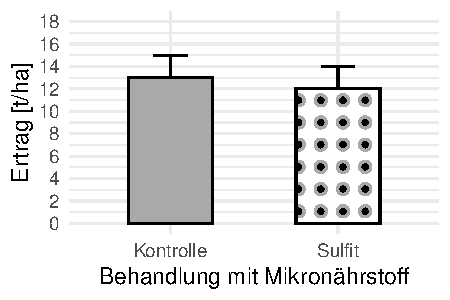
\includegraphics[width=\maxwidth]{img/mc-testing-ttest-02-1} 

}







\begin{enumerate}
\item [\textbf{A} \msquare] Es liegt ein signifikanter Unterschied vor. Der Effekt liegt bei -0.7.
\item [\textbf{B} \msquare] Die Barplots deuten auf keinen signifikanten Unterschied. Der Effekt liegt vermutlich bei -7. Wir müssen aber einen Posthoc-Test rechnen um den Effekt wirklich bestimmen zu können.
\item [\textbf{C} \msquare] Der Test deutet auf einen signifikanten Unterschied hin. Der Effekt liegt vermutlich bei -7.
\item [\textbf{D} \msquare] Es liegt kein signifikanter Unterschied vor. Der Effekt liegt bei -7.
\item [\textbf{E} \msquare] Die Barplots deuten auf einen signifikanten Unterschied. Der Effekt liegt vermutlich bei -7 unter einer groben Abschätzung. Wir müssen aber eine ANOVA rechnen um den Effekt wirklich bestimmen zu können.
\end{enumerate}

\section{Aufgabe \hfill (2 Punkte)}




Sie rechnen einen gepaarten t-Test, da Ihre Beobachtungen verbunden sind. Welche der folgenden Aussagen ist richtig?



\begin{enumerate}
\item [\textbf{A} \msquare] Der gepaarte t-Test nutzt die Varianz der Beobachtungen jeweils paarweise und bildet dafür eine verbundene Stichprobe. Dieser Datensatz $d$ dient dann zur Differenzbildung.
\item [\textbf{B} \msquare] Abhängige Beobachtungen müssen gesondert in einem gepaarten t-Test modelliert werden. Wenn wiederholt an dem gleichen Tier oder Pflanze gemessen wird, dann bilden wir den Quotienten zwischen den beiden Zeitpunkten. Auf den Quotienten rechnen wir den gepaarten t-Test.
\item [\textbf{C} \msquare] Der gepaarte t-Test wird gerechnet, wenn die Beobachtungen nicht unabhängig voneinander sind. Wir messen wiederholt an dem gleichen Probanden oder Tier oder Pflanze. Wir bilden die Differenzen um den gepaarten t-Test rechnen zu können.
\item [\textbf{D} \msquare] Der gepaarte t-Test wird gerechnet, wenn die Beobachtungen abhängig voneinander sind. Wir messen jede Beobachtung nur einmal und berechnen dann die Differenz zu dem Mittel der anderen Beobachtungen.
\item [\textbf{E} \msquare] Beim gepaarten t-Test kombinieren wir die Vorteile des Student t-Test für Varianzhomogenität mit den Vorteilen des Welch t-Test für Varianzheterogenität. Wir bilden dafür die Differenz der Einzelbeobachtungen.
\end{enumerate}

\section{Aufgabe \hfill (2 Punkte)}



In Ihrer Abschlussarbeit passen die Ergebnisse einer ANOVA und eines multiplen Vergleiches nicht zusammen. Nach einem Experiment mit drei Maissorten ergibt eine ANOVA ($p = 0.045$). Sie führen anschließend die paarweisen t-Tests für alle Vergleiche durch. Nach der Adjustierung für multiples Testen ist kein p-Wert unter der $\alpha$-Schwelle. Sie schauen sich auch die rohen, unadjustierten p-Werte an und finden hier als niedrigsten p-Wert $p_{3-2} = 0.052$. Welche Aussage ist richtig?




\begin{enumerate}
\item [\textbf{A} \msquare] Der Fehler liegt in den t-Tests. Wenn eine ANOVA signifikant ist, dann muss zwangsweise auch ein t-Test signifikant sein.
\item [\textbf{B} \msquare] Das Beispiel kann so nicht auftreten, da die ANOVA und die t-Tests algorithmisch miteinander verschränkt sind.
\item [\textbf{C} \msquare] Die ANOVA testet auf der gesamten Fallzahl. Die einzelnen t-Tests immer nur auf einer kleineren Subgruppe. Da mit weniger Fallzahl weniger signifikante Ergebnisse zu erwarten sind, kann eine Diskrepenz zwischen der ANOVA und den paarweisen t-Tests auftreten.
\item [\textbf{D} \msquare] Das ist kein Wunder. Die ANOVA testet nicht auf der gesamten Fallzahl und die paarweisen t-Tests gewinnen immer eine oder mehr Gruppen als Fallzahl dazu. Mit steigender Fallzahl sind mehr signifikante Unterschiede zu erwarten. Die p-Werte unterscheiden sich numerisch auch kaum.
\item [\textbf{E} \msquare] Hier kommt der Effekt der stiegenden Fallzahl auf die Anzahl an signifikante Ergebnisse zu tragen. Da die ANOVA auf weniger Fallzahl testet als die paarweisen t-Tests, kann die ANOVA schwerer einen signifikanten Unterscheid nachweisen.
\end{enumerate}
    
% -----------------------------------------------------------------------
\clearpage
% -----------------------------------------------------------------------
\part{Deskriptive Statistik \& Explorative Datenanalyse}
% -----------------------------------------------------------------------

\section{Aufgabe \hfill (8 Punkte)}

\textit{Geben Sie grundsätzlich Formeln und Rechenweg zur Lösung der Teilaufgaben mit an!} \\[1Ex]
 

 
%% --------------------------------------------------------------------
\begin{minipage}[t]{0.5\textwidth}

\includegraphics[width = 1.3cm]{/Users/kruppajo/work/GitHub/exam/avatare/Mark.png}
\end{minipage}
\begin{minipage}[t]{0.5\textwidth}
\hfill
\href{https://youtu.be/t0WYa_LVc5o}{
\includegraphics[width = 2cm]{img/youtube}}
\end{minipage}
\vspace{-3ex}
%% --------------------------------------------------------------------



\paragraph{Zerforschen des Barplots}

Barplots sind bedeutend in der Darstellung von wissenschaftlichen Ergebnissen. Leider hat sich Mark nicht gemerkt, welche statistischen Maßzahlen für einen Barplot erhoben werden müssen. Besser wäre was anderes gewesen. Geocaching. Ein wunderbares Hobby um sich drin zu verlieren und Abstand zu bekommen. Mark denkt gerne über Geocaching nach. Das ist in soweit doof, da nach seiner Betreuer erstmal ein Barplot nachgebaut werden soll, bevor es mit seinem Projektbericht losgeht. Dann hat er schonmal den \Rlogo Code vorliegen und nachher geht dann alles schneller. Na dann mal los. Mark schafft sich die nötige Stimmung. Mark nickt im Takt von Andrea Berg und bemerkt dabei gar nicht was der Hamster schon wieder anstellt. In der Behandlung für Kartoffeln werden verschiedene Bewässerungstypen ($low$, $mid$ und $high$) sein. Erfasst wird als Endpunkt ($Y$) \textit{Ertrag}. Mark soll dann \textit{yield} in seiner Exceldatei eintragen.



{\centering 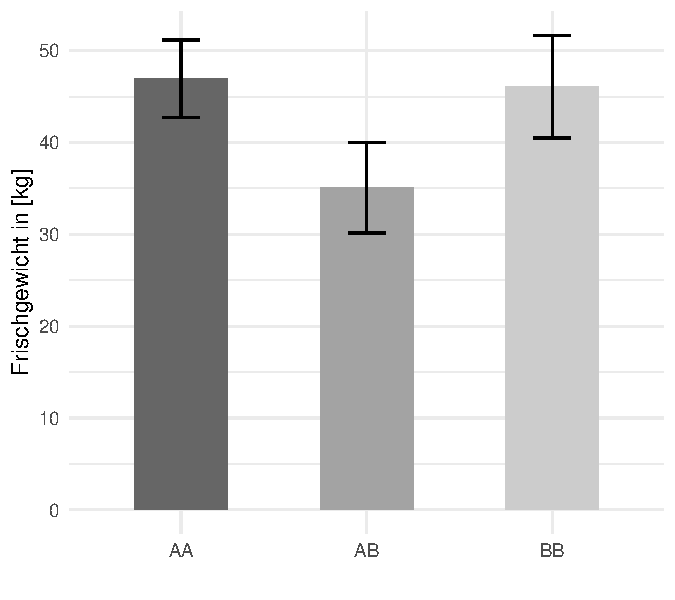
\includegraphics[width=\maxwidth]{img/barplot-02-1} 

}




Leider kennt sich Mark mit der Erstellung von Barplots in \Rlogo nicht aus. Deshalb braucht er bei der Visualisierung Ihre Hilfe!

\begin{enumerate}
\item Formulieren Sie die wissenschaftliche Fragestellung! \textbf{(1 Punkt)}
\item Erstellen Sie eine Tabelle mit den statistischen Maßzahlen der drei Barplots! \textit{Beachten Sie die korrekte Darstellungsform der statistischen Maßzahlen!} \textbf{(3 Punkte)}
\item Erstellen Sie einen beispielhaften Datensatz im \Rlogo üblichen Format, aus dem die drei Barplots \textit{möglicherweise} erstellt wurden! \textbf{(2 Punkte)}
\item Kann Mark einen Unterschied zwischen den Behandlungen erwarten? Begründen Sie Ihre Antwort! \textbf{(2 Punkte)}
\end{enumerate} 
\clearpage
% -----------------------------------------------------------------------

\section{Aufgabe \hfill (8 Punkte)}

\textit{Geben Sie grundsätzlich Formeln und Rechenweg zur Lösung der Teilaufgaben mit an!} \\[1Ex]
 

 
%% --------------------------------------------------------------------
\begin{minipage}[t]{0.5\textwidth}

\includegraphics[width = 1.3cm]{/Users/kruppajo/work/GitHub/exam/avatare/Tina.png}
\end{minipage}
\begin{minipage}[t]{0.5\textwidth}
\hfill
\href{https://youtu.be/vXnLttRL_VI}{
\includegraphics[width = 2cm]{img/youtube}}
\end{minipage}
\vspace{-3ex}
%% --------------------------------------------------------------------



\paragraph{Visualisierung des Barplots}


Barplots sind bedeutend in der Darstellung von wissenschaftlichen Ergebnissen. Leider hat sich Tina nicht gemerkt, welche statistischen Maßzahlen für einen Barplot erhoben werden müssen. Besser wäre was anderes gewesen. Tina liebt Astronomie. Darin kann sie sich wirklich verlieren und immer wieder neu begeistern. Das ist in soweit doof, da nach ihrem Betreuer nun Barplots aus ihren Daten gebaut werden sollen, bevor es mit dem statistischen Testen weitergeht. Na dann mal los. Tina schafft sich die nötige Stimmung. Wenn Tocotronic ertönt, dann sucht die Spinne schleunigst Schutz unter dem Sofa. Tina schüttelt den Kopf. Die Behandlung für Kartoffeln waren verschiedene Düngestufen ($ctrl$, $low$ und $high$). Erfasst wurde von Tina als Messwert ($Y$) \textit{Frischegewicht}. Tina hat dann \textit{freshmatter} in ihrer Exceldatei eintragen. Aber auch irgendwie egal. Einfach mal raus um zu Boxen. Ohne Ziel und Uhr. Das ist was für Tina.

\begin{table}[!h]
\centering
\begin{tabular}{cc}
\toprule
treatment & freshmatter\\
\midrule
low & 49.4\\
ctrl & 31.6\\
high & 36.8\\
low & 39.0\\
low & 44.6\\
\addlinespace
high & 50.6\\
ctrl & 29.1\\
high & 42.9\\
ctrl & 30.5\\
\bottomrule
\end{tabular}
\end{table}



Leider kennt sich Tina mit der Erstellung von Barplots nicht aus. Deshalb braucht sie bei der Visualisierung Ihre Hilfe!

\begin{enumerate}
\item Formulieren Sie die wissenschaftliche Fragestellung! \textbf{(1 Punkt)}
\item Zeichnen Sie in \textit{einer} Abbildung die Barplots für die Behandlung von Kartoffeln! Beschriften Sie die Achsen entsprechend!\textbf{(4 Punkte)}
\item Beschriften Sie \textit{einen} Barplot mit den gängigen statistischen Maßzahlen! \textbf{(2 Punkte)}
\item Wenn Tina \textit{keinen Effekt} zwischen den Behandlungen von Kartoffeln erwarten würde, wie sehen dann die Barplots aus? \textit{Antworten Sie mit einer Skizze der Barplots!}
  \textbf{(1 Punkt)}
\end{enumerate} 
\clearpage
% -----------------------------------------------------------------------

\section{Aufgabe \hfill (9 Punkte)}

\textit{Geben Sie grundsätzlich Formeln und Rechenweg zur Lösung der Teilaufgaben mit an!} \\[1Ex]
 

 
%% --------------------------------------------------------------------
\begin{minipage}[t]{0.5\textwidth}

\includegraphics[width = 1.3cm]{/Users/kruppajo/work/GitHub/exam/avatare/Tina.png}
\end{minipage}
\begin{minipage}[t]{0.5\textwidth}
\hfill
\href{https://youtu.be/Xf0yE-o7bEU}{
\includegraphics[width = 2cm]{img/youtube}}
\end{minipage}
\vspace{-3ex}
%% --------------------------------------------------------------------



\paragraph{Zerforschen des Boxplots}

Tina und die Wut, eine unendliche Geschichte mit kniffeligen Wendungen. Deshalb gilt anschauen, was andere vor einem gemacht haben. Für Tina ist es eine Möglichkeit schneller ans Ziel zu gelangen. Tina soll in ihrer Hausarbeit Brokoli untersuchen. Die Behandlung in ihrer Hausarbeit werden verschiedene Genotypen ($AA$, $AB$ und $BB$) sein. Erheben wird Tina als Endpunkt ($Y$) \textit{Frischegewicht} benannt als \textit{freshmatter} in ihrer Exceldatei. Von ihrer Betreuerin erhält sie nun folgende Abbildung von Boxplots, die sie erstmal zur Übung nachbauen soll, bevor sie mit dem eigentlichen Versuch beginnt. Aber nur in passender Atmospäre! Hm, lecker Katjes und dazu dann im Hintergrund Indiana Jones laufen lassen.



{\centering 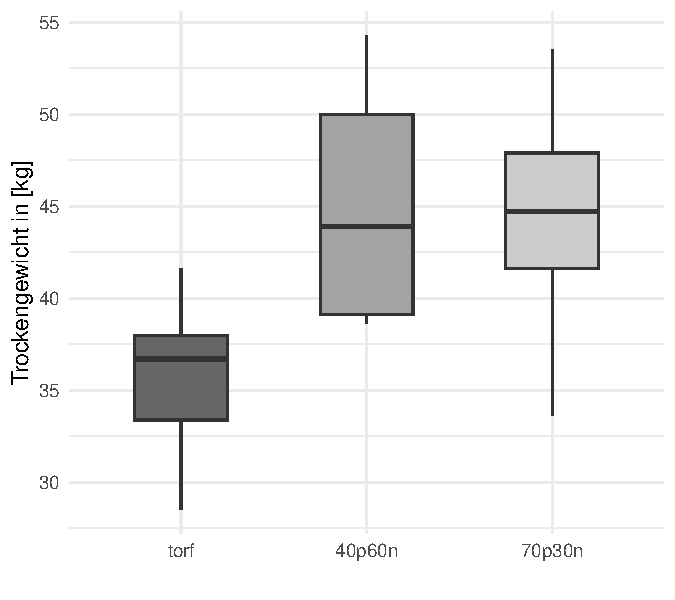
\includegraphics[width=\maxwidth]{img/boxplot-02-zer-1} 

}




Leider kennt sich Tina mit der Erstellung von Boxplots in \Rlogo nicht aus. Deshalb braucht sie bei der Visualisierung Ihre Hilfe!

\begin{enumerate}
\item Erstellen Sie eine Tabelle mit den statistischen Maßzahlen aus der obigen Abbildung der drei Boxplots! \textit{Beachten Sie die korrekte Darstellungsform der statistischen Maßzahlen!} \textbf{(3 Punkte)}
\item Beschriften Sie \textit{einen} der Boxplots mit den gängigen statistischen Maßzahlen! \textbf{(2 Punkte)}
\item Erstellen Sie einen beispielhaften Datensatz, aus dem die drei Boxplots \textit{möglicherweise} erstellt wurden, im \Rlogo üblichen Format! \textbf{(2 Punkte)}
\item Kann Tina einen Unterschied zwischen den Behandlungen erwarten? Begründen Sie Ihre Antwort! \textbf{(2 Punkte)}
\end{enumerate} 
\clearpage
% -----------------------------------------------------------------------

\section{Aufgabe \hfill (9 Punkte)}

\textit{Geben Sie grundsätzlich Formeln und Rechenweg zur Lösung der Teilaufgaben mit an!} \\[1Ex]
 

 
%% --------------------------------------------------------------------
\begin{minipage}[t]{0.5\textwidth}

\includegraphics[width = 1.3cm]{/Users/kruppajo/work/GitHub/exam/avatare/Tina.png}
\end{minipage}
\begin{minipage}[t]{0.5\textwidth}
\hfill
\href{https://youtu.be/0xc0jIPeiyw}{
\includegraphics[width = 2cm]{img/youtube}}
\end{minipage}
\vspace{-3ex}
%% --------------------------------------------------------------------



\paragraph{Visualisierung des Boxplots}

Boxplots sind bedeutend in der Darstellung von wissenschaftlichen Ergebnissen. Leider hat sich Tina nicht gemerkt, welche statistischen Maßzahlen für einen Boxplot erhoben werden müssen. Besser wäre was anderes gewesen. Astronomie. Ein wunderbares Hobby um sich drin zu verlieren und Abstand zu bekommen. Tina denkt gerne über Astronomie nach. Das ist in soweit doof, da nach ihrer Betreuerin nun Boxplots aus ihren Daten gebaut werden sollen, bevor es mit dem statistischen Testen weitergeht. Anhand von Boxplots lässt sich eine Aussage über die Normalverteilung von $Y$ treffen. Die Behandlung für Maiss waren verschiedene Düngestufen ($ctrl$ und $high$). Erfasst wurde von Tina als Endpunkt ($Y$) \textit{Proteingehalt}. Tina hat dann \textit{protein} in ihrer Exceldatei eintragen. Aber nur in passender Atmospäre! Hm, lecker Katjes und dazu dann im Hintergrund Indiana Jones laufen lassen.

\begin{table}[!h]
\centering
\begin{tabular}{cc}
\toprule
treatment & drymatter\\
\midrule
ctrl & 22.0\\
high & 33.6\\
ctrl & 24.4\\
high & 42.1\\
high & 34.0\\
\addlinespace
high & 29.2\\
ctrl & 34.6\\
high & 37.8\\
ctrl & 30.2\\
high & 36.2\\
\addlinespace
ctrl & 26.9\\
high & 36.8\\
high & 31.0\\
ctrl & 26.5\\
ctrl & 35.1\\
\addlinespace
ctrl & 30.8\\
ctrl & 27.4\\
ctrl & 31.6\\
\bottomrule
\end{tabular}
\end{table}



Leider kennt sich Tina mit der Erstellung von Boxplots nicht aus. Deshalb braucht sie bei der Visualisierung Ihre Hilfe!

\begin{enumerate}
\item Zeichnen Sie in \textit{einer} Abbildung die beiden Boxplots für die zwei Behandlungen von Maiss! Beschriften Sie die Achsen entsprechend! \textbf{(5 Punkte)} 
\item Wie ist Ihr Vorgehen, wenn Sie eine \textit{gerade} Anzahl an
  Beobachtungen pro Gruppe haben? \textbf{(1 Punkt)}
\item Beschriften Sie \textit{einen} der beiden Boxplots mit den gängigen
  statistischen Maßzahlen! \textbf{(2 Punkte)}
\item Wenn Sie \textit{keinen Effekt} zwischen den Behandlungen von
  Maiss erwarten würden, wie sehen dann die beiden Boxplots aus?
  \textit{Antworten Sie mit einer Skizze der Boxplots!}
  \textbf{(1 Punkt)}
\end{enumerate} 
\clearpage
% -----------------------------------------------------------------------

\section{Aufgabe \hfill (8 Punkte)}

\textit{Geben Sie grundsätzlich Formeln und Rechenweg zur Lösung der Teilaufgaben mit an!} \\[1Ex]
 

 
%% --------------------------------------------------------------------
\begin{minipage}[t]{0.5\textwidth}

\includegraphics[width = 1.3cm]{/Users/kruppajo/work/GitHub/exam/avatare/Yuki.png}
\end{minipage}
\begin{minipage}[t]{0.5\textwidth}
\hfill
\href{https://youtu.be/aXvxGC4YLqk}{
\includegraphics[width = 2cm]{img/youtube}}
\end{minipage}
\vspace{-3ex}
%% --------------------------------------------------------------------



\paragraph{Visualisierung des Histogramm für kategoriale Daten}

Yuki schmeißt noch eine Handvoll Reese's Peanut Butter Cups in ihren Rachen. Im Hintergrund klirrt leise der Spiegel zum Sound von London Grammar. Yuki betrachtet die folgenden Daten nach einem Versuch in einer Klimakammer mit Kartoffeln. In dem Experiment wurden die seltsamen Verdickungen gezählt. Nach der Meinung ihrem Betreuer muss als erstes geschaut werden, wie diese verteilt sind. Also welcher statistischen Verteilung die seltsamen Verdickungen folgen. Dazu soll Yuki ein Histogramm verwenden. Dann hätte man auch einen guten Überblick über den Messwert ($Y$). Es wäre einfacher, wenn da nicht noch was wäre. Wenn die Faulheit nicht wäre, ja dann wäre wohl vieles möglich für Yuki! Aber so.. Yuki streichelt liebevoll das Minischwein. Der Kopf ist in ihrem Schloß vergraben um den Klang von London Grammar zu dämpfen.

\begin{center}
Die seltsamen Verdickungen: 5, 3, 2, 3, 2, 5, 4, 2, 4, 3, 6, 7, 6, 2, 6, 8, 4, 3, 1, 7, 5, 1, 3, 2, 2, 7, 7, 6, 7, 4, 4, 2, 4
\end{center}

Leider kennt sich Yuki mit der Erstellung von Histogrammen überhaupt nicht aus. Deshalb braucht sie bei der Erstellung Ihre Hilfe!

\begin{enumerate}
\item Zeichen Sie ein Histogramm um die Verteilung der Daten zu visualisieren! (\textbf{3 Punkte})
\item Beschriften Sie die Achsen der Abbildung! (\textbf{2 Punkte})
\item Ergänzen Sie die absoluten und relativen Häufigkeiten in der
  Abbildung! \textbf{(1 Punkt)}
\item Berechnen Sie aus den Daten die \textit{Wahrscheinlichkeit}
  gleich oder mehr als die Anzahl 5 zu beobachten! \textbf{(1
    Punkt)}
\item Berechnen Sie aus den Daten die \textit{Chance} gleich oder mehr
  als die Anzahl 5 zu beobachten! \textbf{(1 Punkt)}
\end{enumerate}

 
\clearpage
% -----------------------------------------------------------------------

\section{Aufgabe \hfill (8 Punkte)}

\textit{Geben Sie grundsätzlich Formeln und Rechenweg zur Lösung der Teilaufgaben mit an!} \\[1Ex]
 

 
%% --------------------------------------------------------------------
\begin{minipage}[t]{0.5\textwidth}

\includegraphics[width = 1.3cm]{/Users/kruppajo/work/GitHub/exam/avatare/Paula.png}
\end{minipage}
\begin{minipage}[t]{0.5\textwidth}
\hfill
\href{https://youtu.be/ORHSPTCdfeY}{
\includegraphics[width = 2cm]{img/youtube}}
\end{minipage}
\vspace{-3ex}
%% --------------------------------------------------------------------



\paragraph{Visualisierung des Histogramm für kontinuierliche Daten}

Paula schmeißt noch eine Handvoll Smarties in ihren Rachen. Im Hintergrund klirrt leise der Spiegel zum Sound von White Lies. Paula betrachtet die folgenden Daten nach einem Gewächshausexperiment mit Spargel. In dem Experiment wurden die mittleren seltsamen Verdickungen gezählt. Nach der Meinung ihrer Betreuerin muss als erstes geschaut werden, wie diese verteilt sind. Also welcher statistischen Verteilung die mittleren seltsamen Verdickungen folgen. Dazu soll Paula ein Histogramm verwenden. Dann hätte man auch einen guten Überblick über das Outcome ($Y$). Es wäre einfacher, wenn da nicht noch was wäre. Eine echte Herausforderung für sie war schon immer der Perfektionismus gewesen. Ein leidiges Lied. Paula nickt im Takt von White Lies und bemerkt dabei gar nicht was die Ratte schon wieder anstellt.

\begin{center}
Die mittleren seltsamen Verdickungen: 8, 11.2, 10.9, 11.3, 7.5, 10.7, 11.7, 8.8, 13.2, 7.5, 7.8, 9, 9.2, 10.8, 7.9, 8.7, 12.5, 9.5, 10.1, 11.4, 10, 11, 11.6, 9.5, 15.2
\end{center}

Leider kennt sich Paula mit der Erstellung von Histogrammen überhaupt nicht aus. Deshalb braucht sie bei der Erstellung Ihre Hilfe!

\begin{enumerate}
\item Zeichen Sie ein Histogramm um die Verteilung der Daten zu visualisieren! (\textbf{3 Punkte})
 \item Erläutern Sie Ihr Vorgehen um ein Histogramm für kontinuierliche Daten zu zeichnen!  (\textbf{2 Punkte})
\item Beschriften Sie die Achsen der Abbildung! (\textbf{2 Punkte})
\item Ergänzen Sie die relativen Häufigkeiten in der Abbildung! \textbf{(1 Punkt)}  
\end{enumerate}

 
\clearpage
% -----------------------------------------------------------------------

\section{Aufgabe \hfill (10 Punkte)}

\textit{Geben Sie grundsätzlich Formeln und Rechenweg zur Lösung der Teilaufgaben mit an!} \\[1Ex]
 

 
%% --------------------------------------------------------------------
\begin{minipage}[t]{0.5\textwidth}

\includegraphics[width = 1.3cm]{/Users/kruppajo/work/GitHub/exam/avatare/Mark.png}
\end{minipage}
\begin{minipage}[t]{0.5\textwidth}
\hfill
\href{https://youtu.be/VAqiUdV4WQ0}{
\includegraphics[width = 2cm]{img/youtube}}
\end{minipage}
\vspace{-3ex}
%% --------------------------------------------------------------------




\paragraph{Visualisierung des Scatterplots}

Mark liest laut: 'Wenn zwei kontinuierliche Variablen vorliegen, können diese in einer exploartiven Datenanalyse...'. Mark stoppt. Mark schmeißt noch eine Handvoll Marzipankugeln in seinen Rachen. Im Hintergrund klirrt leise der Spiegel zum Sound von Andrea Berg. Was waren noch gleich kontinuierliche Variablen? In seiner Hausarbeit hatte er ein Freilandversuch im Emsland durchgeführt. Dabei ging es um den Zusammenhang zwischen Frischegewicht [kg/ha] und durchschnittliche UV Einstrahlung [UV/d] im groben Kontext von Brokkoli. Nun stellt sich die Frage für ihn, ob es überhaupt einen Zusammenhang zwischen den gemessenen Variablen gibt. Dafür war eine explorative Datenanalyse gut! Wenn die Unsicherheit nicht wäre, ja dann wäre wohl vieles möglich für Mark! Aber so.. Dann was anderes. Wenn Columbo läuft, dann ist der Hamster nicht mehr da. Aber jetzt braucht er mal Entspannung!

\begin{table}[!h]
\centering
\begin{tabular}{cc}
\toprule
Durchschnittliche UV Einstrahlung [UV/d] & Frischegewicht [kg/ha]\\
\midrule
26.5 & 38.9\\
24.5 & 37.0\\
22.6 & 36.1\\
25.7 & 40.5\\
22.5 & 32.4\\
\addlinespace
22.9 & 32.2\\
23.1 & 37.5\\
30.6 & 41.3\\
24.1 & 34.1\\
22.1 & 33.7\\
\addlinespace
25.7 & 37.2\\
\bottomrule
\end{tabular}
\end{table}



Leider kennt sich Mark mit der Erstellung einer explorativen Datenanalyse für kontinuierliche Daten überhaupt nicht aus. Deshalb braucht er bei der Erstellung Ihre Hilfe!

\begin{enumerate}
\item Erstellen Sie eine Visualisierung für die Datentabelle. Beschriften Sie
  die Achsen entsprechend! \textbf{(4 Punkte)}
\item Schätzen Sie eine Gerade durch die Punkte! \textbf{(1 Punkt)}
\item Beschriften Sie die Gerade mit den gängigen statistischen Maßzahlen! Geben Sie die numerischen Zahlenwerte mit an! \textbf{(3 Punkte)}
\item Wenn \textit{kein} Effekt von $x$ auf $y$ vorhanden wäre, wie würde die Gerade verlaufen und welche Werte würden die statistischen Maßzahlen annehmen? \textbf{(2 Punkt)}
\end{enumerate} 
\clearpage
% -----------------------------------------------------------------------

\section{Aufgabe \hfill (10 Punkte)}

\textit{Geben Sie grundsätzlich Formeln und Rechenweg zur Lösung der Teilaufgaben mit an!} \\[1Ex]
 

 
%% --------------------------------------------------------------------
\begin{minipage}[t]{0.5\textwidth}

\includegraphics[width = 1.3cm]{/Users/kruppajo/work/GitHub/exam/avatare/Mark.png}
\end{minipage}
\begin{minipage}[t]{0.5\textwidth}
\hfill
\href{https://youtu.be/t_1KL77mfmg}{
\includegraphics[width = 2cm]{img/youtube}}
\end{minipage}
\vspace{-3ex}
%% --------------------------------------------------------------------



\paragraph{Visualisierung des Mosaicplots}

In ein Feldexperiment in der Uckermark hatte Mark sich zum einen die Behandlung Herbizideinsatz [ja/nein] und zum anderen die Messung Trockengewicht über Zielwert [ja/nein] im Kontext von Maiss angeschaut. Nun steht Mark vor dem Problem, dass er zwei kategoriale Variablen in seinem Projektbericht gemessen hat. Dazu kommt dann noch was anderes. Eine echte Herausforderung für ihn war schon immer die Unsicherheit gewesen. Ein leidiges Lied. Da sein Betreuer erstmal die langen Tabellen mit ja/nein in einer explorativen Datenanalyse zusammengefasst und präsentiert bekommen möchte bevor es überhaupt weitergeht, muss er jetzt eine Lösung finden. Was alles auch nicht einfacher macht. Am liebsten würde er ja was anderes machen. Geocaching. Ein wunderbares Hobby um sich drin zu verlieren und Abstand zu bekommen. Mark denkt gerne über Geocaching nach.



\vspace{1Ex}

\begin{center}
\begin{minipage}[t]{0.45\textwidth}
%\small
\begin{center}

\begin{tabular}{p{2.5cm}p{2.5cm}p{2.5cm}p{2.5cm}}
\toprule
Herbizideinsatz & Trockengewicht über Zielwert\\
\midrule
ja & ja\\
nein & nein\\
nein & nein\\
nein & nein\\
ja & nein\\
\addlinespace
nein & nein\\
nein & nein\\
ja & ja\\
ja & ja\\
nein & ja\\
\addlinespace
nein & nein\\
nein & nein\\
ja & nein\\
ja & nein\\
nein & ja\\
\addlinespace
nein & ja\\
ja & nein\\
\bottomrule
\end{tabular}


\end{center}
\end{minipage}
\begin{minipage}[t]{0.45\textwidth}
%\small
\begin{center}

\begin{tabular}{p{2.5cm}p{2.5cm}p{2.5cm}p{2.5cm}}
\toprule
Herbizideinsatz & Trockengewicht über Zielwert\\
\midrule
ja & nein\\
nein & ja\\
nein & nein\\
ja & ja\\
ja & nein\\
\addlinespace
ja & ja\\
nein & nein\\
ja & nein\\
ja & ja\\
nein & ja\\
\addlinespace
nein & nein\\
ja & nein\\
ja & nein\\
ja & nein\\
ja & nein\\
\addlinespace
ja & nein\\
nein & nein\\
\bottomrule
\end{tabular}


\end{center}
\end{minipage}
\end{center}

\vspace{2Ex}

Leider kennt sich Mark mit der Erstellung einer explorativen Datenanalyse für kategoriale Daten überhaupt nicht aus. Deshalb braucht er bei der Erstellung Ihre Hilfe!

\begin{enumerate}
\item Stellen Sie den Zusammenhang zwischen den beiden kategorialen Variablen in einer zusammenfassenden Tabelle dar! \textbf{(3 Punkte)}
\item Visualisieren Sie den Zusammenhang zwischen den beiden kategorialen Variablen! \textbf{(3 Punkte)}
\item Berechnen Sie die Verhältnisse in der Visualisierung! Welche Annahme haben Sie getroffen? \textbf{(2 Punkte)}
\item Wenn \textit{kein} Effekt von der Behandlung vorliegen würde, wie würde die Tabelle und die Visualisierung aussehen? \textbf{(2 Punkt)}
\end{enumerate} 
\clearpage
% -----------------------------------------------------------------------

\section{Aufgabe \hfill (10 Punkte)}

\textit{Geben Sie grundsätzlich Formeln und Rechenweg zur Lösung der Teilaufgaben mit an!} \\[1Ex]
 

 
%% --------------------------------------------------------------------
\begin{minipage}[t]{0.5\textwidth}

\includegraphics[width = 1.3cm]{/Users/kruppajo/work/GitHub/exam/avatare/Steffen.png}\hspace{-4mm}
\includegraphics[width = 1.3cm]{/Users/kruppajo/work/GitHub/exam/avatare/Yuki.png}
\end{minipage}
\begin{minipage}[t]{0.5\textwidth}
\hfill
\href{https://youtu.be/Op-gjzASH9I}{
\includegraphics[width = 2cm]{img/youtube}}
\end{minipage}
%% --------------------------------------------------------------------



\paragraph{Visualisierung von Verteilungen}

'Was soll das denn jetzt schon wieder sein? Drei Boxplot, die auf der Seite liegen?', entfährt es Yuki und schaut dabei Steffen an. 'Keine Ahnung. Es ist bestimmt wieder so ein Lernziel mit der Verteilung und so.', meint Steffen sichtlich genervt und mampft noch ein paar Oreos. 'Du weißt doch wie es heißt, \textit{Frei ist, wer missfallen kann.}\footnote{Oschmann, A. (2024) Mädchen stärken: Stärken fördern, Selbstwert erhöhen und liebevoll durch Krisen begleiten. Goldegg Verlag}', merkt Yuki nickend an. Die beiden schauen angestrengt auf die drei Boxplots. Das Ziel ist es zu verstehen, wie eine Verteilung anhand eines Boxplots bewertet werden kann. Steffen und die Faulheit machen die Sache nicht einfacher.



{\centering 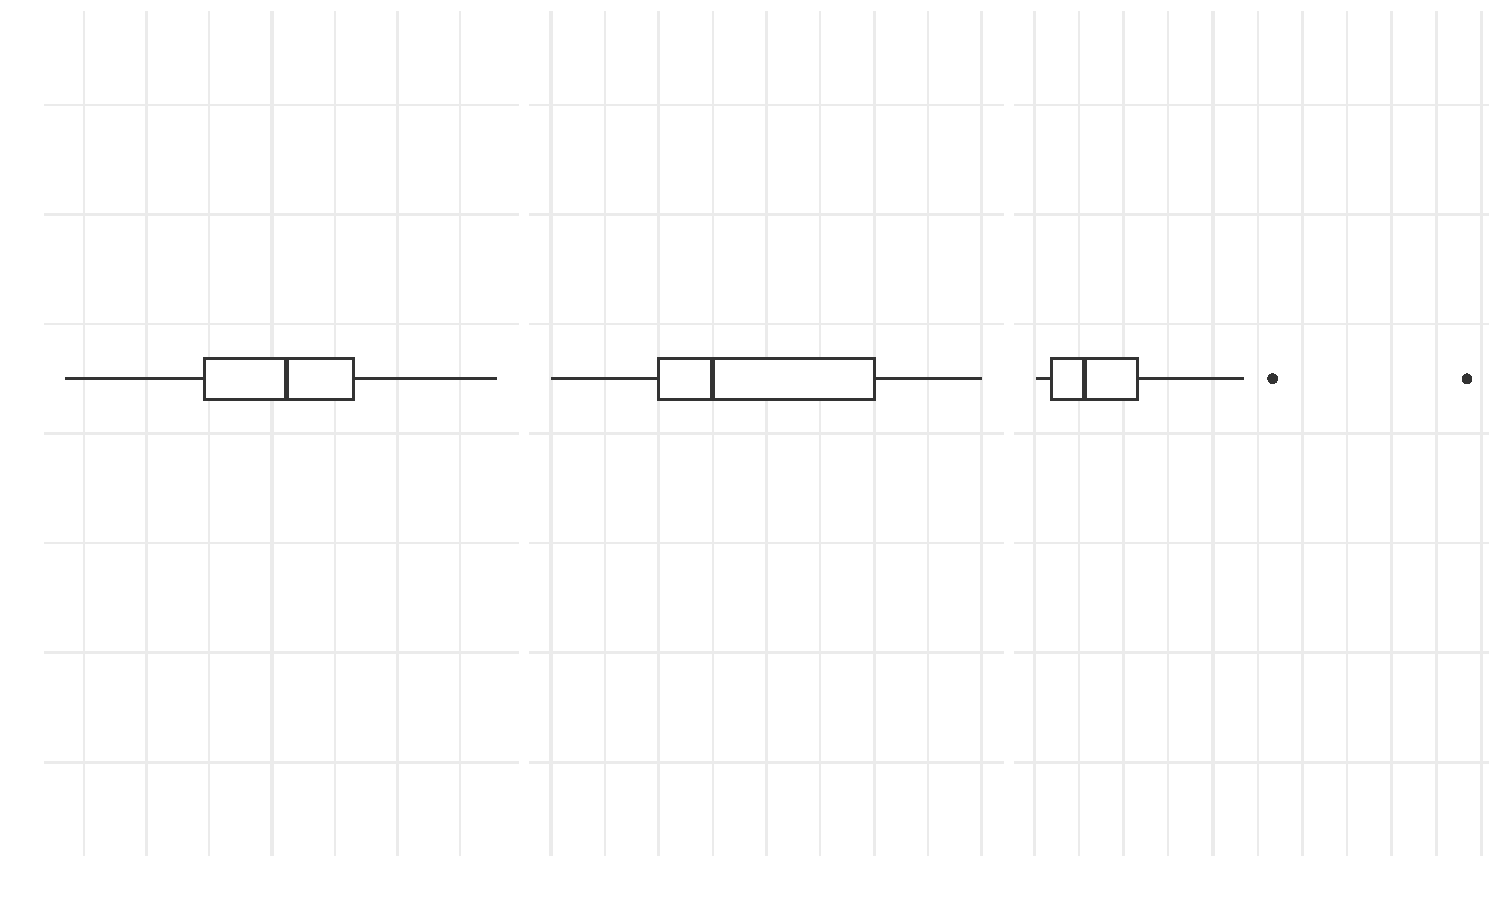
\includegraphics[width=\maxwidth]{img/desc-stat-11-1} 

}




Jetzt brauchen Yuki und Steffen Ihre Hilfe bei der Abschätzung einer Verteilung anhand von Boxplots um ihre Arbeit dann in diesem Semester noch abschließen zu können.

\begin{enumerate}
\item Zeichnen Sie über die Boxplots die entsprechende zugehörige Verteilung! \textbf{(3 Punkte)} 
\item Zeichnen Sie unter die Boxplots die entsprechende zugehörige Beobachtungen als Stiche! \textbf{(3 Punkte)}
\item Wie viel Prozent der Beobachtungen fallen in das IQR? Ergänzen Sie die Abbildung entsprechend um den Bereich! \textbf{(2 Punkte)}
\item Wie viel Prozent der Beobachtungen fallen in $\bar{y} \pm 1s$ und $\bar{y} \pm 2s$  unter der Annahme einer Normalverteilung? \textbf{(2 Punkte)}
\end{enumerate} 
\clearpage
% -----------------------------------------------------------------------

\section{Aufgabe \hfill (10 Punkte)}

\textit{Geben Sie grundsätzlich Formeln und Rechenweg zur Lösung der Teilaufgaben mit an!} \\[1Ex]
 

 
%% --------------------------------------------------------------------
\begin{minipage}[t]{0.5\textwidth}

\includegraphics[width = 1.3cm]{/Users/kruppajo/work/GitHub/exam/avatare/Alex.png}\hspace{-4mm}
\includegraphics[width = 1.3cm]{/Users/kruppajo/work/GitHub/exam/avatare/Jonas.png}
\end{minipage}
\begin{minipage}[t]{0.5\textwidth}
\hfill
\href{https://youtu.be/ZrJhn2wPbq4}{
\includegraphics[width = 2cm]{img/youtube}}
\end{minipage}
%% --------------------------------------------------------------------



\paragraph{Visualisierung der Normalverteilung}

Alex und die Gefälligkeit machen die Sache mit dem Studium nicht einfacher. Immerhin ist noch Jonas zur Hilfe mit dabei. Jonas hat Gummibärchen mitgebracht und Abba aufgedreht. Das ist immerhin eine Ablenkung. Nicht so gut wie Starcraft, aber immerhin etwas. Jetzt sollen die beiden diese komische Aufgabe lösen. Es geht um verschiedene Normalverteilungen. Anscheinend hängen Normalverteilungen vom Mittelwert $\bar{y}$ und der Standardabweichung $s$ ab. 'Wozu brauchen wir nochmal Normalverteilungen?', entfährt es Alex. Durch das Mampfen von Jonas versteht er kein Wort der Antwort. Jonas lächelt.\\



Jetzt brauchen Alex und Jonas Ihre Hilfe bei der Abschätzung einer Verteilung um ihre Arbeit dann in diesem Semester noch abschließen zu können.

\begin{enumerate}
\item Skizzieren Sie zwei Normalverteilungen mit $\bar{y}_1 \neq \bar{y}_2$ und $s_1 \neq s_2$! \textbf{(3 Punkte)}
\item Beschriften Sie die Normalverteilungen mit den statistischen Maßzahlen! \textbf{(2 Punkte)}
\item Liegt Varianzhomogenität oder Varianzheterogenität vor? Begründen Sie Ihre Antwort! \textbf{(2 Punkte)}
\item In welchen Bereich fallen 68\% bzw. 95\% der Beobachtungen in einer Normalverteilung? Ergänzen Sie die Bereiche in \underline{einer} Normalverteilung! \textbf{(2 Punkte)}
\item Ergänzen Sie unter \underline{einer} der Normalverteilungen den entsprechenden Boxplot! \textbf{(1 Punkt)}
\end{enumerate}

 
\clearpage
% -----------------------------------------------------------------------

\section{Aufgabe \hfill (10 Punkte)}

\textit{Geben Sie grundsätzlich Formeln und Rechenweg zur Lösung der Teilaufgaben mit an!} \\[1Ex]
 

 
%% --------------------------------------------------------------------
\begin{minipage}[t]{0.5\textwidth}

\includegraphics[width = 1.3cm]{/Users/kruppajo/work/GitHub/exam/avatare/Steffen.png}\hspace{-4mm}\includegraphics[width = 1.3cm]{/Users/kruppajo/work/GitHub/exam/avatare/Tina.png}
\end{minipage}
\begin{minipage}[t]{0.5\textwidth}
\hfill
\href{https://youtu.be/MiD42k4l5Ag}{\includegraphics[width = 2cm]{img/youtube}}
\end{minipage}
%% --------------------------------------------------------------------



\paragraph{Visualisierung der Normalverteilung und der Poissonverteilung}

'Was sollen wir hier dann noch zeichnen?!', entfährt es Steffen und schaut dabei Tina an. 'Wir sollen eine Normalverteilung mit einem Mittelwert von $\bar{y}_1 = 2$ und einer Standardabweichung von $s_1 = 1$ zeichnen. Sowie eine weitere Normalverteilung mit einem Mittelwert von $\bar{y}_2 = 0$ und einer Standardabweichung von $s_2 = 1$. Keine Ahnung wie das geht. Darunter sollen dann noch eine Poissonverteilung mit einem Mittelwert von $\lambda_1 = 15$ sowie einer weiteren Poissonverteilung mit einem Mittelwert von $\lambda_2 = 1$ gezeichnet werden.', meint Tina sichtlich genervt und mampft noch ein paar Katjes. Im Hintergrund spielt leise Tocotronic. 'Wirre Geschichte...', merkt Steffen nickend an. Die beiden schauen angestrengt auf die leeren Flächen für die Abbildungen. Tina und die Romantik machen die Suche nach der Lösung nicht einfacher.\\




{\centering \includegraphics[width=\maxwidth]{img/histogram-01-1} 

}




Jetzt brauchen Steffen und Tina Ihre Hilfe bei der Abschätzung einer Verteilung um ihre Arbeit dann in diesem Semester noch abschließen zu können.


\begin{enumerate}
\item Skizzieren Sie die zwei Normalverteilungen und zwei Poissonverteilungen! \textbf{(4 Punkte)}
\item Achten Sie auf die entsprechende Skalierung in den jeweiligen Abbildungen! \textbf{(2 Punkte)}
\item Ergänzen Sie unter \underline{einer} Normalverteilung den entsprechenden Boxplot! \textbf{(1 Punkt)}
\item Ergänzen Sie unter \underline{einer} Poissonverteilung den entsprechenden Boxplot! \textbf{(1 Punkt)}
\item Geben Sie ein Beispiel für ein Outcome $y$, welches einer Normalverteilung folgt! \textbf{(1 Punkt)}
\item Geben Sie ein Beispiel für ein Outcome $y$, welches einer Poissonverteilung folgt! \textbf{(1 Punkt)}
\end{enumerate} 
\clearpage
% -----------------------------------------------------------------------
\part{Statistisches Testen \& statistische Testtheorie}
% -----------------------------------------------------------------------  

\section{Aufgabe \hfill (9 Punkte)}


 
%% --------------------------------------------------------------------
\begin{minipage}[t]{0.5\textwidth}
\includegraphics[width = 1.3cm]{/Users/kruppajo/work/GitHub/exam/avatare/Paula.png}\hspace{-4mm}\includegraphics[width = 1.3cm]{/Users/kruppajo/work/GitHub/exam/avatare/Steffen.png}
\end{minipage}
\begin{minipage}[t]{0.5\textwidth}
\hfill
\href{https://youtu.be/aHVYuFKTqZs}{\includegraphics[width = 2cm]{img/youtube}}
\end{minipage}
%% --------------------------------------------------------------------



\paragraph{Grundgesamtheit und experimentelle Stichprobe}

'Schnapspraline?', räuspert sich das Känguruh und schaukelt in der Wippe. Steffen und Paula schauen erschrocken auf. 'Ähm, das ist hier eine Klausuraufgabe...', merkt Steffen mit leicht schrägen Blick an. 'Ich mache hier ein Praktikum und schreibe Teile der Aufgaben.', gähnt das Känguruh. 'Also, ich glaube das ist so nicht gedacht. Und das sind die Schnapspralinen für den Geburtstag meiner Oma!', ruft Paula. 'Pillepalle! Meins, deins, das sind doch alles bürgerliche Kategorien!', entgegnet das Känguruh und liest von einem zerknitterten Stück Papier ab: 'Was ist der Unterschied zwischen dem Einen und dem Anderen. Steht alles unten in den Fragen. Einfach selber lesen...'.

\vspace{1ex}

Leider kennen sich Steffen und Paula mit der Grundgesamtheit und der Stuchprobe überhaupt nicht aus. Daher sind Sie gefragt!

\begin{enumerate}
\item Nennen Sie das statistische Verfahren und zwei konkrete Beispiele zur Durchführung um von einer Grundgesamtheit auf eine Stichprobe zu gelangen! \textbf{(3 Punkte)}
\item Erklären Sie den Zusammenhang zwischen Stichprobe und Grundgesamtheit an einem Schaubild! Beschriften Sie das Schaubild entsprechend!
  \textit{Nutzen Sie hierfür als Veranschaulichung die Körpergröße von Männern oder Frauen aus den Gummibärchendaten!}  \textbf{(3 Punkte)}
\item Erweitern Sie das Schaubild um die Entstehung von $Pr(D|H_0)$! \textit{Nutzen Sie hierfür als Veranschaulichung zusätzlich die Gruppierungsvariable "`Modul"' aus den Gummibärchendaten!}  \textbf{(3 Punkte)}
\end{enumerate} 
\clearpage
% -----------------------------------------------------------------------

\section{Aufgabe \hfill (9 Punkte)}


 
%% --------------------------------------------------------------------
\begin{minipage}[t]{0.5\textwidth}
\includegraphics[width = 1.3cm]{/Users/kruppajo/work/GitHub/exam/avatare/Alex.png}\hspace{-4mm}\includegraphics[width = 1.3cm]{/Users/kruppajo/work/GitHub/exam/avatare/Paula.png}
\end{minipage}
\begin{minipage}[t]{0.5\textwidth}
\hfill
\href{https://youtu.be/Ric8ne39DtI}{\includegraphics[width = 2cm]{img/youtube}}
\end{minipage}
%% --------------------------------------------------------------------



\paragraph{Das Nullritual - Die statistische Testtheorie}

'Fechten ist der beste Sport, den es gibt.', meint Paula. Alex entgegnet, ' Ich empfehle ja immer allen Laufen.' Die beiden sind im Zoo und diskutieren, ob Pinguine Knie haben. Eigentlich wollten beide nochmal die statistische Testheorie durchgehen, sind dann aber auf abenteuerlichen Wege im Zoo gelandet. Paula starrt wie hypnotisiert auf einen strullenden Elefanten und stopt die Zeit.\footnote{Yang, P. J., et al. (2014). Duration of urination does not change with body size. Proceedings of the National Academy of Sciences, 111(33), 11932-11937.} 'Du bist so peinlich.', entfährt es Alex.

\vspace{1ex}

Leider kennen sich Paula und Alex mit statistischen Testtheorie, auch Null-Ritual genannt, überhaupt nicht aus. Geschweige denn mit der Visualisierung als Kreuztabelle.  

\begin{enumerate}
\item Tragen Sie folgende statistische Fachbegriffe zur statistischen Testtheorie korrekt eine selbst erstellte Kreuztabelle ein! \textbf{(3 Punkte)}
  \begin{center}
  \begin{tabular}{cccc}
  H$_0$ beibehalten & H$_0$ wahr & 20\% & H$_0$ falsch \\
  \end{tabular}
  \end{center}
\item Ergänzen Sie Ihre erstellte Kreuztabelle um vier weitere, passende Fachbegriffe zur statistischen Testtheorie! \textbf{(2 Punkte)}
\end{enumerate}

Die Entscheidungsfindung durch einen statistischen Test kann auch durch die Analogie zu einem Feuermelder abgebildet werden. Dabei symbolisiert der Feuermelder den statistischen Test und es soll getestet werden, ob ein Feuer ausgebrochen ist.

\begin{enumerate}
  \setcounter{enumi}{2}    
\item In der Analogie des Feuermelders, wie lautet der $\alpha$-Fehler? \textbf{(1 Punkt)}
\item In der Analogie des Feuermelders, wie lautet der $\beta$-Fehler? \textbf{(1 Punkt)}
\item Wenn der Feuermelder einmal pro Tag messen würde, wie oft würde der Feuermelder mit einem $\alpha$ von 5\% in einem Monat Alarm schlagen? Begründen Sie Ihre Antwort! \textbf{(2 Punkte)}
\end{enumerate}



 
\clearpage
% -----------------------------------------------------------------------

\section{Aufgabe \hfill (9 Punkte)}

\textit{Geben Sie grundsätzlich Formeln und Rechenweg zur Lösung der Teilaufgaben mit an!} \\[1Ex]


 
%% --------------------------------------------------------------------
\begin{minipage}[t]{0.5\textwidth}
\includegraphics[width = 1.3cm]{/Users/kruppajo/work/GitHub/exam/avatare/Alex.png}\hspace{-4mm}\includegraphics[width = 1.3cm]{/Users/kruppajo/work/GitHub/exam/avatare/Yuki.png}
\end{minipage}
\begin{minipage}[t]{0.5\textwidth}
\hfill
\href{https://youtu.be/32JjH1eyuTU}{\includegraphics[width = 2cm]{img/youtube}}
\end{minipage}
%% --------------------------------------------------------------------



\paragraph{Visualisierung der Teststatistik $\boldsymbol{T_D}$ und dem p-Wert}

'Wir sollen die Teststatistik $T_D$ umd dem p-Wert visualisieren, da mit einer Visualisierung vieles verständlicher wird!', ruft Alex um Abba zu übertönen. 'Ich weiß nicht, was das jetzt helfen soll. Können wir nicht einfach schauen, ob der p-Wert kleiner als das Signifikanzniveau  $\alpha$ gleich 5\% ist? Und gut ist?', merkt Yuki an, was aber im Refrain von Abba untergeht. Alex nickt im Beat. 'Wir haben hier eine t-verteilung unter der Annahme der Nullhypothese!', singt er.

\vspace{1ex}

Leider kennen sich Alex und Yuki mit der Visualisierung der Teststatistik $T_D$ und dem p-Wert überhaupt nicht aus und brauchen dahr Ihre Hilfe!

\vspace{1ex}

\textit{Beachten Sie, dass im Folgenden \underline{keine numerisch korrekte Darstellung} verlangt wird! Es gilt Erkennbarkeit vor Genauigkeit!}

\begin{enumerate}
\item Ergänzen Sie eine beschriftete $x$-Achse! \textbf{(1 Punkt)}
\item Ergänzen Sie "`$\bar{y}_1 = \bar{y}_2$"'! \textbf{(1 Punkt)} 
\item Ergänzen Sie "`$A = 0.95$"'! \textbf{(1 Punkt)}
\item Zeichnen Sie $T_{\alpha=5\%}$ in die Abbildung! \textbf{(1 Punkt)} 
\item Zeichnen Sie das Signifikanzniveau $\alpha$ in die Abbildung! Begründen Sie Ihre Antwort! \textbf{(2 Punkte)} 
\item Zeichnen Sie $-T_{D}$ in die Abbildung! \textbf{(1 Punkt)}
\item Zeichnen Sie einen signifikant p-Wert in die Abbildung! Begründen Sie Ihre Antwort! \textbf{(2 Punkte)}   
\end{enumerate}



{\centering \includegraphics[width=\maxwidth]{img/statistisches-testen-3-1} 

}


 
\clearpage
% -----------------------------------------------------------------------

\section{Aufgabe \hfill (10 Punkte)}


 
%% --------------------------------------------------------------------
\begin{minipage}[t]{0.5\textwidth}
\includegraphics[width = 1.3cm]{/Users/kruppajo/work/GitHub/exam/avatare/Jessica.png}\hspace{-4mm}\includegraphics[width = 1.3cm]{/Users/kruppajo/work/GitHub/exam/avatare/Tina.png}
\end{minipage}
\begin{minipage}[t]{0.5\textwidth}
\hfill
\href{https://youtu.be/CN_O4fYPbhs}{\includegraphics[width = 2cm]{img/youtube}}
\end{minipage}
%% --------------------------------------------------------------------



\paragraph{Visualisierung des 95\% Konfidenzintervalls}

'So, was haben wir gemacht? Wir haben einen t-test für den Vergleich der Mittelwerte gerechnet.', meint Jessica. Tina schaut fragend. 'Hatten wir nicht alles zu einer Kontrolle verglichen? Das war doch so!', ruft Tina laut aus. 'Wir haben doch Messwert \textit{Chlorophyllgehalt nach Subsitution} erhoben.', stellt Jessica fest. Jetzt haben beide das Problem, die möglichen 95\% Konfidenzintervalle zu interpretieren.

\vspace{1ex}

Leider kennen sich Jessica und Tina mit der Visualisierung des 95\% Konfidenzintervall überhaupt nicht aus. 

\begin{enumerate}
\item Beschriften Sie die untenstehende Abbildung mit der Signifikanzschwelle! Begründen Sie Ihre Antwort! \textbf{(2 Punkte)}
\item Ergänzen Sie eine \textit{in den Kontext passende} Relevanzschwelle! Begründen Sie Ihre Antwort! \textbf{(2 Punkte)} 
\item Skizieren Sie in die untenstehende Abbildung sechs einzelne Konfidenzintervalle (a-f) mit den
  jeweiligen Eigenschaften! \textbf{(6 Punkte)}
  \begin{itemize}
  \item[(a)] Ein signifikantes, relevantes 95\% Konfidenzintervall 	
  \item[(b)] Ein 95\% Konfidenzintervall mit niedriger Varianz $s_p$ in der Stichprobe als der Rest 95\% der Konfidenzintervalle 	
  \item[(c)] Ein signifikantes, relevantes 99\% Konfidenzintervall. 	
  \item[(d)] Ein nicht signifikantes, nicht relevantes 95\% Konfidenzintervall 
  \item[(e)] Ein 95\% Konfidenzintervall mit h{"o}herer Varianz $s_p$ in der Stichprobe als der Rest der 95\% Konfidenzintervalle
  \item[(f)] Ein signifikantes, nicht relevantes 95\% Konfidenzintervall
  \end{itemize}
\end{enumerate}

\begin{center}
  \includegraphics[height = 10cm]{/Users/kruppajo/work/GitHub/exam/question/img/statistisches-testen-04}
\end{center}


 
\clearpage
% -----------------------------------------------------------------------

\section{Aufgabe \hfill (10 Punkte)}

\textit{Geben Sie grundsätzlich Formeln und Rechenweg zur Lösung der Teilaufgaben mit an!} \\[1Ex]


 
%% --------------------------------------------------------------------
\begin{minipage}[t]{0.5\textwidth}
\includegraphics[width = 1.3cm]{/Users/kruppajo/work/GitHub/exam/avatare/Alex.png}\hspace{-4mm}\includegraphics[width = 1.3cm]{/Users/kruppajo/work/GitHub/exam/avatare/Mark.png}
\end{minipage}
\begin{minipage}[t]{0.5\textwidth}
\hfill
\href{https://youtu.be/FgZmpnEWDag}{\includegraphics[width = 2cm]{img/youtube}}
\end{minipage}
%% --------------------------------------------------------------------



\paragraph{Zusammenhang zwischen dem Effekt, der Streuung sowie der Fallzahl}

An einem kalten Dezembermorgen haben sich Alex und Mark zum Lernen verabredet. Eine große Kanne Tee und Berge von Gummibärchen warten darauf gegessen zu werden. Alex liest laut vor:\begin{quote}
                 \textit{
                 Beim statistischen Testen gibt es einen Zusammenhang zwischen dem Effekt, der Streuung sowie der Fallzahl. Gegeben sei die Formel für den Student t-Test auf den die folgenden Überlegungen basieren sollen. Welche Auswirkung hat die Änderungen der jeweiligen statistischen Maßzahl des Effekts $\Delta$, der Streuung $s$ und der Fallzahl $n$ auf die Teststistik $T_{D}$, den p-Wert $Pr(D|H_0)$ sowie dem Konfidenzintervall $KI_{1-\alpha}$?
                 }
                 \end{quote}Mark hebt die Augenbraue. 'Irgendwie sagt mir die Aufgabe jetzt mal so gar nichts. Was soll da gemacht werden?', merkt Mark an und ergänzt: 'Schauen wir doch erstmal zur Entspannung Columbo, den Film habe ich extra nochmal mitgebracht.' Alex ist der Idee nicht abgeneigt und auch die Katze kommt unter dem Sofa hervor um mitzuschauen. 

\vspace{1ex}

Leider kennen sich Alex und Mark mit dem Zusammenhang zwischen dem Effekt, der Streuung sowie der Fallzahl überhaupt nicht aus. 


\begin{enumerate}
\item Visualisieren Sie den Zusammenhang zwischen der Teststatiatik $T_{D}$ und dem p-Wert $Pr(D|H_0)$ für sich verändernde $T_{D}$-Werte!\textit{Geben Sie dafür ein numerisches Beispiel in dem Sie drei $T_{D}$-Werte und deren Einfluss auf den p-Wert vergleichen!} \textbf{(3 Punkte)}  
\item  Füllen Sie die untenstehende Tabelle aus in dem Sie die Änderung der statistischen Maßzahlen auf die Teststatistik, den p-Wert sowie das Konfidenzintervall in \textit{einem} Wort oder Symbol beschreiben! \textbf{(4 Punkte)}
\begin{center}
  \large
  \begin{tabular}[c]{l|c|c|c|l|c|c|c}
    & $T_{D}$ & $Pr(D|H_0)$ & $KI_{1-\alpha}$ & & $T_{D}$ & $Pr(D|H_0)$ & $KI_{1-\alpha}$\strut\\ 
    \hline
    \textbf{$\Delta\; \uparrow$} & \hspace{1.8cm} & \hspace{1.8cm}  & \hspace{1.8cm} & \textbf{
                                                          $\Delta\; \downarrow$} &
                                                                          \hspace{1.8cm} & \hspace{1.8cm}  & \hspace{1.8cm}\strut\\
    \hline
        \textbf{$s\; \uparrow$} & \hspace{1.8cm} & \hspace{1.8cm}  & \hspace{1.8cm} & \textbf{
                                                          $s\; \downarrow$} &
                                                                          \hspace{1.8cm}
                                                & \hspace{1.8cm}  & \hspace{1.8cm}\strut\\
    \hline
        \textbf{$n\; \uparrow$} & \hspace{1.8cm} & \hspace{1.8cm}  & \hspace{1.8cm} & \textbf{
                                                          $n\; \downarrow$} &
                                                                          \hspace{1.8cm}
                                                & \hspace{1.8cm}  & \hspace{1.8cm}\strut\\
    \hline
  \end{tabular}
\end{center}
\item Visualisieren Sie ein 95\%-iges Konfidenzintervall im Vergleich zu einem 90\%-igen Konfidenzintervall! Begründen Sie Ihre Visualisierung anhand der Formel des Konfidenzintervalls des t-Tests mathematisch! \textbf{(3 Punkte)} 
\end{enumerate} 
\clearpage
% -----------------------------------------------------------------------
\part{Der Student t-Test, Welch t-Test \& gepaarter t-Test}
% -----------------------------------------------------------------------

\section{Aufgabe \hfill (9 Punkte)}

\textit{Geben Sie grundsätzlich Formeln und Rechenweg zur Lösung der Teilaufgaben mit an!} \\[1Ex]
 

 
%% --------------------------------------------------------------------
\begin{minipage}[t]{0.5\textwidth}
\includegraphics[width = 1.3cm]{/Users/kruppajo/work/GitHub/exam/avatare/Mark.png}
\end{minipage}
\begin{minipage}[t]{0.5\textwidth}
\hfill
\href{https://youtu.be/eejS2uG4o-M}{\includegraphics[width = 2cm]{img/youtube}}
\end{minipage}
\vspace{-3ex}
%% --------------------------------------------------------------------



\paragraph{Berechnung des Student t-Test \underline{oder} Welch t-Test}

Mark ist im Emsland für einen Pilotexperiment mit sehr geringer Fallzahl $(n_1 = n_2 = 3)$ mit Hühnern. Allein diese Tatsache ist für ihn eine Erzählung wert. Eine echte Herausforderung für ihn war schon immer die Unsicherheit gewesen. Ein leidiges Lied.  Für seiner Hausarbeit musste er ein Kreuzungsexperiment mit Hühnern durchführen und das sollte laut seinem Betreuer an diesem Ort besonders gut gelingen, da man hier gut neue technische Anlagen und Behandlungen fernab der Bevölkerung testen könne. Zeugen gibt es hier jedenfalls keine. Gar keine.  Alleine sein hilft jetzt aber nur bedingt, denn seine Behandlung Flüssignahrung ($ctrl$ und $flOw$) und der Messwert Fettgehalt [\%/kg] sollen mit einem t-Test ausgewertet werden. Immerhin weiß er, dass sein Messwert einer Normalverteilung folgt. Hm..., was entspannendes wäre gut. Mark will später nochmal raus um zu Reiten. Druck ablassen, dass muss er auch.

\begin{table}[!h]
\centering
\begin{tabular}{cc}
\toprule
treatment & weight\\
\midrule
dose & 11.0\\
ctrl & 12.2\\
ctrl & 15.2\\
dose & 17.4\\
dose & 15.6\\
\addlinespace
ctrl & 13.1\\
\bottomrule
\end{tabular}
\end{table}



Leider kennt sich Mark mit der Berechnung eines t-Tests überhaupt nicht aus. Deshalb braucht er bei der Berechnung Ihre Hilfe!

\begin{enumerate}
  \item Formulieren Sie das statistische Hypothesenpaar! \textbf{(1 Punkt)}
  \item Bestimmen Sie die Teststatistik $T_{D}$ eines Student t-Tests! \textbf{(3 Punkte)}
  \item Treffen Sie mit $T_{\alpha = 5\%} = 2.04$ eine Aussage zur Nullhypothese! Begründen Sie Ihre Antwort! \textbf{(2 Punkte)}
  \item Berechnen Sie den Effekt des Student t-Tests! \textbf{(1 Punkt)}
  \item Formulieren Sie eine Antwort an Mark über das Ergebnis Ihrer statistischen Analyse! \textbf{(2 Punkte)}
\end{enumerate} 
\clearpage
% -----------------------------------------------------------------------

\section{Aufgabe \hfill (12 Punkte)}

\textit{Geben Sie grundsätzlich Formeln und Rechenweg zur Lösung der Teilaufgaben mit an!} \\[1Ex]
 

 
%% --------------------------------------------------------------------
\begin{minipage}[t]{0.5\textwidth}
\includegraphics[width = 1.3cm]{/Users/kruppajo/work/GitHub/exam/avatare/Yuki.png}
\end{minipage}
\begin{minipage}[t]{0.5\textwidth}
\hfill
\href{https://youtu.be/Cq_rF_z4xOk}{\includegraphics[width = 2cm]{img/youtube}}
\end{minipage}
\vspace{-3ex}
%% --------------------------------------------------------------------



\paragraph{Berechnung des Student t-Test}

Der t-Test. Yuki erschaudert. Eine echte Herausforderung für sie war schon immer die Faulheit gewesen. Ein leidiges Lied. Ein mächtiges Werkzeug ist der t-Test in den Händen desjenigen, der einen normalverteilten Messwert ($Y$) hat. Aber erstmal überhaupt den t-Test rechnen können. Wie sah das Experiment von Yuki überhaupt aus? Yuki schmeißt noch eine Handvoll Reese's Peanut Butter Cups in ihren Rachen. Im Hintergrund klirrt leise der Spiegel zum Sound von London Grammar. Yuki hat ein Kreuzungsexperiment mit Zandern durchgeführt. Dabei wurde die Behandlung Ernährungszusatz ($ctrl$ und $fedX$) an den Zandern getestet. Gemessen hat Yuki dann als Messwert Schlachtgewicht [kg]. Warum der Versuch in der Uckermark für ihre Abschlussarbeit stattfinden musste, ist ihr bis heute ein Rätsel. Egal. Gibt es jetzt einen Zusammenhang zwischen der Behandlung und Schlachtgewicht [kg]?

\begin{table}[!h]
\centering
\begin{tabular}{cc}
\toprule
Ernährungszusatz & Schlachtgewicht\\
\midrule
fedX & 17.3\\
fedX & 12.9\\
ctrl & 37.9\\
ctrl & 37.8\\
fedX & 42.3\\
\addlinespace
ctrl & 38.1\\
fedX & 36.0\\
fedX & 28.9\\
ctrl & 35.4\\
ctrl & 38.3\\
\addlinespace
fedX & 40.9\\
fedX & 11.2\\
fedX & 21.8\\
ctrl & 40.4\\
ctrl & 45.6\\
\bottomrule
\end{tabular}
\end{table}



Leider kennt sich Yuki mit der Berechnung eines t-Tests überhaupt nicht aus. Deshalb braucht sie bei der Berechnung Ihre Hilfe!

\begin{enumerate}
  \item Formulieren Sie die wissenschaftliche Fragestellung! \textbf{(1 Punkt)}
  \item Formulieren Sie das statistische Hypothesenpaar! \textbf{(1 Punkt)}
  \item Bestimmen Sie die Teststatistik $T_{D}$ eines Student t-Tests! \textbf{(3 Punkte)}
\item Treffen Sie mit $T_{\alpha = 5\%} = 1.84$ eine Aussage zur Nullhypothese! Begründen Sie Ihre Antwort! \textbf{(2 Punkte)}
\item Berechnen Sie den Effekt des Student t-Tests! \textbf{(1 Punkt)}
\item Wenn Sie \textit{keinen} Unterschied zwischen den Behandlungsgruppen erwarten würden, wie groß wäre dann die Teststatistik $T_{D}$? Begründen Sie Ihre Antwort! \textbf{(2 Punkte)}
\item Formulieren Sie eine Antwort an Yuki über das Ergebnis Ihrer statistischen Analyse! \textbf{(2 Punkte)}
\end{enumerate} 
\clearpage
% -----------------------------------------------------------------------

\section{Aufgabe \hfill (12 Punkte)}

\textit{Geben Sie grundsätzlich Formeln und Rechenweg zur Lösung der Teilaufgaben mit an!} \\[1Ex]
 

 
%% --------------------------------------------------------------------
\begin{minipage}[t]{0.5\textwidth}
\includegraphics[width = 1.3cm]{/Users/kruppajo/work/GitHub/exam/avatare/Tina.png}
\end{minipage}
\begin{minipage}[t]{0.5\textwidth}
\hfill
\href{https://youtu.be/TbSEOMCQYl4}{\includegraphics[width = 2cm]{img/youtube}}
\end{minipage}
\vspace{-3ex}
%% --------------------------------------------------------------------



\paragraph{Berechnung des Welch t-Test}


Das Oldenburger Land, unendliche Weiten. Wir schreiben das Jahr 2024. Dies sind die Abenteuer von Tina, die mit ihrer 1 Frau starken Besatzung 12 Wochen lang unterwegs ist, um neue Welten zu erforschen, neues Leben und neue Zivilisationen. 'Oder nennen wir es Ödnis und Verzweiflung', denkt Tina. Für ihrer Hausarbeit ist Tina ins Nichts gezogen. Tina und die Wut, eine unendliche Geschichte mit kniffeligen Wendungen. Was macht sie nun? Tina hat einen Leistungssteigerungsversuch mit Hühnern durchgeführt. Die Behandlung Genotypen ($AA$ und $BB$) wurde an Hühnern getestet. Gemessen hat sie dann als einen normalverteilten Endpunkt ($Y$) Fettgehalt [\%/kg]. Jetzt soll sie ihrer Betreuerin nach testen, ob die Behandlung Genotypen ($AA$ und $BB$) ein signifikantes Ergebnis liefert. Hm..., was entspannendes wäre gut. Tina schmeißt noch eine Handvoll Katjes in ihren Rachen. Im Hintergrund klirrt leise der Spiegel zum Sound von Tocotronic.

\begin{table}[!h]
\centering
\begin{tabular}{cc}
\toprule
Genotypen & Fettgehalt\\
\midrule
AA & 32.0\\
BB & 53.1\\
BB & 43.6\\
BB & 46.8\\
BB & 44.6\\
\addlinespace
BB & 39.7\\
BB & 59.6\\
AA & 28.7\\
AA & 27.6\\
BB & 44.0\\
\addlinespace
AA & 26.2\\
AA & 31.2\\
AA & 35.0\\
AA & 38.9\\
\bottomrule
\end{tabular}
\end{table}



Leider kennt sich Tina mit der Berechnung eines t-Tests überhaupt nicht aus. Deshalb braucht sie bei der Berechnung Ihre Hilfe!

\begin{enumerate}
  \item Formulieren Sie die wissenschaftliche Fragestellung! \textbf{(1 Punkt)}
  \item Formulieren Sie das statistische Hypothesenpaar! \textbf{(1 Punkt)}
  \item Bestimmen Sie die Teststatistik $T_{D}$ eines  Welch t-Tests! \textbf{(3 Punkte)}
  \item Treffen Sie mit $T_{\alpha = 5\%} = 1.84$ eine Aussage zur Nullhypothese! Begründen Sie Ihre Antwort! \textbf{(2 Punkte)}
\item Berechnen Sie das 95\% Konfidenzintervall. Welche Annahmen haben Sie getroffen? \textbf{(2 Punkte)}
\item Nennen Sie den statistischen Grund, warum Sie sich zwischen einem Student t-Test und einem Welch t-Test entscheiden müssen! \textbf{(1 Punkt)}
\item Formulieren Sie eine Antwort an Tina über das Ergebnis Ihrer statistischen Analyse! \textbf{(2 Punkte)}
\end{enumerate} 
\clearpage
% -----------------------------------------------------------------------

\section{Aufgabe \hfill (11 Punkte)}

\textit{Geben Sie grundsätzlich Formeln und Rechenweg zur Lösung der Teilaufgaben mit an!} \\[1Ex]
 

 
%% --------------------------------------------------------------------
\begin{minipage}[t]{0.5\textwidth}
\includegraphics[width = 1.3cm]{/Users/kruppajo/work/GitHub/exam/avatare/Paula.png}\hspace{-4mm}\includegraphics[width = 1.3cm]{/Users/kruppajo/work/GitHub/exam/avatare/Tina.png}
\end{minipage}
\begin{minipage}[t]{0.5\textwidth}
\hfill
\href{https://youtu.be/QR90zyn0Iz8}{\includegraphics[width = 2cm]{img/youtube}}
\end{minipage}
%% --------------------------------------------------------------------



\paragraph{Berechnung des gepaarten t-Test}

Paula und Tina haben sich dazu entschieden zusammenzuarbeiten. Das sollte alles etwas einfacher machen. Jeder hat zwar ein getrenntes Themenfeld aber den Hauptversuch machen beide gemeinsam. Das hat sich schonmal als gut Idee soweit herausgestellt. In einer Hausarbeit sollen beide herausfinden, ob es einen Zusammenhang zwischen Jäten ($Aussaat$ und $Ernte$) und Proteingehalt [g/kg] gibt. Die Besonderheit ist hierbei, dass die Messungen an der gleichen Beobachtung stattfinden. Beide messen also zweimal an den gleichen Erbsen. Hier muss dann wohl auf einen normalverteilten Endpunkt ($Y$) ein gepaarter t-Test gerechnet werden. Paula schaut etwas flehentlich zu Tina. Wenn der Perfektionismus nicht wäre, ja dann wäre wohl vieles möglich für Paula! Aber so... Steffen denkt derweil angestrengt an Tocotronic und wippt leicht mit dem Fuß.

\begin{table}[!h]
\centering
\begin{tabular}{ccc}
\toprule
ID & treatment & freshmatter\\
\midrule
6 & Aussaat & 25.0\\
1 & Aussaat & 14.9\\
4 & Ernte & 55.8\\
8 & Aussaat & 36.0\\
4 & Aussaat & 16.4\\
\addlinespace
1 & Ernte & 35.6\\
2 & Aussaat & 29.7\\
7 & Ernte & 51.2\\
2 & Ernte & 52.2\\
6 & Ernte & 41.6\\
\addlinespace
3 & Ernte & 59.9\\
5 & Ernte & 44.3\\
7 & Aussaat & 33.9\\
3 & Aussaat & 45.5\\
5 & Aussaat & 31.6\\
\bottomrule
\end{tabular}
\end{table}



Leider kennen sich Paula und Tina mit der Berechnung eines gepaarten t-Tests überhaupt nicht aus. Deshalb brauchen sie beide bei der Berechnung Ihre Hilfe!

\begin{enumerate}
  \item Formulieren Sie die wissenschaftliche Fragestellung! \textbf{(1 Punkt)}
  \item Formulieren Sie das statistische Hypothesenpaar! \textbf{(1 Punkt)}
  \item Bestimmen Sie die Teststatistik $T_{D}$ eines gepaarten t-Tests! \textbf{(3 Punkte)}
  \item Treffen Sie mit $T_{\alpha = 5\%} = 1.84$ eine Aussage zur Nullhypothese! Begründen Sie Ihre Antwort! \textbf{(2 Punkte)}
\item Schätzen Sie den $p$-Wert des gepaarten t-Tests ab! Begründen Sie Ihre Antwort mit einer Skizze! \textbf{(2 Punkte)}
\item Formulieren Sie eine Antwort an Paula über das Ergebnis Ihrer statistischen Analyse! \textbf{(2 Punkte)}
\end{enumerate}


 
\clearpage
% -----------------------------------------------------------------------

\section{Aufgabe \hfill (10 Punkte)}

\textit{Geben Sie grundsätzlich Formeln und Rechenweg zur Lösung der Teilaufgaben mit an!} \\[1Ex]
 

 
%% --------------------------------------------------------------------
\begin{minipage}[t]{0.5\textwidth}
\includegraphics[width = 1.3cm]{/Users/kruppajo/work/GitHub/exam/avatare/Alex.png}\hspace{-4mm}\includegraphics[width = 1.3cm]{/Users/kruppajo/work/GitHub/exam/avatare/Paula.png}\hspace{-4mm}\includegraphics[width = 1.3cm]{/Users/kruppajo/work/GitHub/exam/avatare/Tina.png}
\end{minipage}
\begin{minipage}[t]{0.5\textwidth}
\hfill
\href{https://youtu.be/exDo7AyHl4Q}{\includegraphics[width = 2cm]{img/youtube}}
\end{minipage}
%% --------------------------------------------------------------------



\paragraph{Interpretation des t-Tests in \Rlogo - die Teststatistik und der p-Wert}


Tina und Alex sind bei Paula um sich Hilfe in \Rlogo zu holen.  Im Hintergrund wummert White Lies. Die beiden hatten zwar schon erste Kontakte mit \Rlogo sind sich aber unsicher bei der Interpetierung der Ausgabe eines t-Tests für ihren gemeinsamen Versuch. Es würde auch besser funktionieren, wenn Paula nicht der Perfektionismus im Weg stehen würde und Tina nicht das Problem hätte die Wut zu händeln. In einem Projektbericht haben beide zusammen Puten untersucht. Dabei ging es um den Zusammenhang zwischen der Behandlung Bestandsdichte ($Verordnung$ und $Erhöht$) und dem Messwert Protein/Fettrate [\%/kg]. Der Versuch wurde in einem Leistungssteigerungsversuch im Teuteburgerwald durchgeführt. Nach des Betreuers ist der Messwert Protein/Fettrate [\%/kg] normalverteilt und ein t-Test passt daher. Das wird jetzt nicht mehr angezweifel...Paula überlegt, ob sie die beiden nicht noch auf den Film \textit{Jagd auf roter Oktober} einlädt.

\begin{knitrout}
\definecolor{shadecolor}{rgb}{0.969, 0.969, 0.969}\color{fgcolor}\begin{kframe}
\begin{verbatim}
## 
## 	Two Sample t-test
## 
## data:  Protein/Fettrate by Bestandsdichte
## t = 0.60243, df = 14, p-value = 0.5565
## alternative hypothesis: true  is not equal to [condensed]
## 95 percent confidence interval:
##  -4.596241  8.186717
## sample estimates:
## mean in group Verordnung     mean in group Erhöht 
##                 45.42857                 43.63333
\end{verbatim}
\end{kframe}
\end{knitrout}

Helfen Sie Paula bei der Interpretation des t-Tests! Sonst geht es auch für Tina und Alex nicht weiter.
  
\begin{enumerate}
  \item Formulieren Sie die wissenschaftliche Fragestellung! \textbf{(1 Punkt)}
  \item Formulieren Sie das statistische Hypothesenpaar! \textbf{(1 Punkt)}
\item Liegt ein signifikanter Unterschied zwischen den Gruppen vor? Begründen Sie Ihre Antwort! \textbf{(2 Punkte)}
\item Skizzieren Sie eine Abbildung in der Sie $T_{D}$, $Pr(D|H_0)$, $A=0.95$, sowie $T_{\alpha=5\%} = |2.14|$ einzeichnen! \textbf{(4 Punkte)}
\item Beschriften Sie die Abbildung! \textbf{(1 Punkt)}  
\item Berechnen Sie den Effekt des t-Tests! \textbf{(1 Punkt)}
\end{enumerate} 
\clearpage
% -----------------------------------------------------------------------

\section{Aufgabe \hfill (10 Punkte)}

\textit{Geben Sie grundsätzlich Formeln und Rechenweg zur Lösung der Teilaufgaben mit an!} \\[1Ex]
 

 
%% --------------------------------------------------------------------
\begin{minipage}[t]{0.5\textwidth}
\includegraphics[width = 1.3cm]{/Users/kruppajo/work/GitHub/exam/avatare/Jonas.png}\hspace{-4mm}\includegraphics[width = 1.3cm]{/Users/kruppajo/work/GitHub/exam/avatare/Nilufar.png}\hspace{-4mm}\includegraphics[width = 1.3cm]{/Users/kruppajo/work/GitHub/exam/avatare/Steffen.png}
\end{minipage}
\begin{minipage}[t]{0.5\textwidth}
\hfill
\href{https://youtu.be/wJqsNV1hOW8}{\includegraphics[width = 2cm]{img/youtube}}
\end{minipage}
%% --------------------------------------------------------------------



\paragraph{Interpretation des t-Tests in \Rlogo - das 95\% Konifidenzintervall}


'Mit dem R Paket \texttt{\{emmeans\}} können wir gleich die Gruppenvergleiche rechnen und uns das \textit{compact letter displac}' ausgeben lassen!', verkündet Jonas sichtlich stolz. Ein paar Mal hat sie schon die Erschöpfung gehindert weiterzumachen. 'Nach Meinung der Betreuerin soll es aber nur erstmal ein t-Test sein. Und die Ausgabe ist schon wirr genug.', merkt Nilufar an. Nilufar und Steffen sind bei Jonas um sich in \Rlogo helfen zu lassen. Im Hintergrund wummert Iron Maiden. Steffen streichelt zur Beruhigung das Meerschweinchen von Jonas. Die beiden waren 3 Monate im Wendland um einen Versuch mit Hühnern in einem Stallexperiment durchzuführen. Ziel war es das Outcome ($Y$) Fettgehalt [\%/kg] zu bestimmen. Jonas überlegt, ob er die beiden nicht noch auf den Film \textit{Mission Impossible} einlädt oder dann doch lieber raus geht um zu Schwimmen? Vielleicht will ja Steffen mit. Besser als der Film.

\begin{knitrout}
\definecolor{shadecolor}{rgb}{0.969, 0.969, 0.969}\color{fgcolor}\begin{kframe}
\begin{verbatim}
## 
## 	Two Sample t-test
## 
## data:  Fettgehalt by Elterlinie
## t = 7.1395, df = 19, p-value = 8.702e-07
## alternative hypothesis: true  is not equal to [condensed]
## 95 percent confidence interval:
##   9.865516 18.049029
## sample estimates:
## mean in group Standard     mean in group Xray 
##               42.93000               28.97273
\end{verbatim}
\end{kframe}
\end{knitrout}

Helfen Sie Jonas bei der Interpretation des t-Tests! Sonst geht es auch für Nilufar und Steffen nicht weiter.

\begin{enumerate}
  \item Formulieren Sie die wissenschaftliche Fragestellung! \textbf{(1 Punkt)}
  \item Formulieren Sie das statistische Hypothesenpaar! \textbf{(1 Punkt)}
\item Liegt ein signifikanter Unterschied zwischen den Gruppen vor? Begründen Sie Ihre Antwort! \textbf{(2 Punkte)}
\item Skizieren Sie das sich ergebende 95\% Konifidenzintervall! \textbf{(2 Punkte)}
\item Beschriften Sie die Abbildung und das 95\% Konfidenzintervall entsprechend! \textbf{(2 Punkte)}  
\item Interpretieren Sie den Effekt des 95\% Konifidenzintervalls! \textbf{(2 Punkte)}
\end{enumerate} 
\clearpage
% -----------------------------------------------------------------------

\section{Aufgabe \hfill (9 Punkte)}

\textit{Geben Sie grundsätzlich Formeln und Rechenweg zur Lösung der Teilaufgaben mit an!} \\[1Ex]
 

 
%% --------------------------------------------------------------------
\begin{minipage}[t]{0.5\textwidth}
\includegraphics[width = 1.3cm]{/Users/kruppajo/work/GitHub/exam/avatare/Alex.png}\hspace{-4mm}\includegraphics[width = 1.3cm]{/Users/kruppajo/work/GitHub/exam/avatare/Mark.png}\hspace{-4mm}\includegraphics[width = 1.3cm]{/Users/kruppajo/work/GitHub/exam/avatare/Steffen.png}
\end{minipage}
\begin{minipage}[t]{0.5\textwidth}
\hfill
\href{https://youtu.be/w62HJlbN28U}{\includegraphics[width = 2cm]{img/youtube}}
\end{minipage}
%% --------------------------------------------------------------------



\paragraph{Interpretation des t-Tests in \Rlogo - die Visualisierung}

'Mit dem R Paket \texttt{\{emmeans\}} können wir gleich die Gruppenvergleiche rechnen und uns das \textit{compact letter displac}' ausgeben lassen!', verkündet Alex sichtlich stolz. Ein paar Mal hat sie schon die Gefälligkeit gehindert weiterzumachen. 'Nach Meinung des Betreuers soll es aber nur erstmal ein t-Test sein. Und die Ausgabe ist schon wirr genug.', merkt Mark an. Mark und Steffen sind bei Alex um sich in \Rlogo helfen zu lassen. Im Hintergrund wummert Abba. Steffen streichelt zur Beruhigung die Katze von Alex. Die beiden waren 3 Monate im Teuteburgerwald um einen Versuch mit Erdbeeren in einem Gewächshausexperiment durchzuführen. Ziel war es das Outcome ($Y$) Proteingehalt [g/kg] zu bestimmen. Alex überlegt, ob er die beiden nicht noch auf den Film \textit{Alien} einlädt oder dann doch lieber raus geht um zu Laufen? Vielleicht will ja Steffen mit. Besser als der Film.

\begin{knitrout}
\definecolor{shadecolor}{rgb}{0.969, 0.969, 0.969}\color{fgcolor}\begin{kframe}
\begin{verbatim}
## 
## 	Two Sample t-test
## 
## data:  Proteingehalt by Düngestufen
## t = 2.1419, df = 16, p-value = 0.04793
## alternative hypothesis: true  is not equal to [condensed]
## 95 percent confidence interval:
##   0.05542189 10.73418850
## sample estimates:
## mean in group ctrl mean in group high 
##           33.00909           27.61429
\end{verbatim}
\end{kframe}
\end{knitrout}

Helfen Sie Alex bei der Interpretation des t-Tests! Sonst geht es auch für Mark und Steffen nicht weiter.
  
\begin{enumerate}
  \item Formulieren Sie die wissenschaftliche Fragestellung! \textbf{(1 Punkt)}
  \item Formulieren Sie das statistische Hypothesenpaar! \textbf{(1 Punkt)}
\item Liegt ein signifikanter Unterschied zwischen den Gruppen vor? Begründen Sie Ihre Antwort! \textbf{(2 Punkte)}
\item Skizieren Sie die sich ergebenden Boxplot! Welche Annahmen an die Daten haben Sie getroffen? Begründen Sie Ihre
  Antwort! \textbf{(2 Punkte)} 
\item Skizieren Sie die sich ergebenden Barplots! \textbf{(2 Punkte)}
\item Berechnen Sie den Effekt des t-Tests! \textbf{(1 Punkt)}
\end{enumerate}
 
\clearpage
% -----------------------------------------------------------------------

\section{Aufgabe \hfill (10 Punkte)}

\textit{Geben Sie grundsätzlich Formeln und Rechenweg zur Lösung der Teilaufgaben mit an!} \\[1Ex]
 

 
%% --------------------------------------------------------------------
\begin{minipage}[t]{0.5\textwidth}
\includegraphics[width = 1.3cm]{/Users/kruppajo/work/GitHub/exam/avatare/Jessica.png}\hspace{-4mm}\includegraphics[width = 1.3cm]{/Users/kruppajo/work/GitHub/exam/avatare/Nilufar.png}
\end{minipage}
\begin{minipage}[t]{0.5\textwidth}
\hfill
\href{https://youtu.be/kHmfEmU6lrk}{\includegraphics[width = 2cm]{img/youtube}}
\end{minipage}
%% --------------------------------------------------------------------



\paragraph{Interpretation des gepaarten t-Tests in \Rlogo}

Alles voll mit Zandern. Aber das haben Jessica und Nilufar eben gemeinsam in einer Abschlussarbeit gemacht! Worum ging es aber konkret? Beide haben als einen normalverteilten Messwert ($Y$) Gewichtszuwachs in der 1LW von Zandern bestimmt. Die Daten haben beide zusammen in einem Kreuzungsexperiment erhoben. In dem Experiment ging es um eine vorher/nachher Untersuchung an den gleichen Zandern. Als Behandlung wurde Ernährungszusatz ($ohne$ und $14d$) eingesetzt. Nach der Meinung des Betreuers muss hier ein gepaarter t-Test gerechnet werden. Leider kennen sich beide nicht sehr gut in \Rlogo aus. Jessica hat einiges an Schokobons geholt, so dass beide die Zeit gut durchbringen werden. Dann geht Jessica nochmal zum Sport. Jessica will später nochmal raus um Rad zu fahren. Druck ablassen, dass muss sie auch.

\begin{knitrout}
\definecolor{shadecolor}{rgb}{0.969, 0.969, 0.969}\color{fgcolor}\begin{kframe}
\begin{verbatim}
## 
## 	Paired t-test
## 
## data:  Gewichtszuwachs by Ernährungszusatz
## t = 1.3962, df = 8, p-value = 0.2002
## alternative hypothesis: true  is not equal to [condensed]
## 95 percent confidence interval:
##  -4.213602 17.146935
## sample estimates:
## mean difference 
##        6.466667
\end{verbatim}
\end{kframe}
\end{knitrout}

Jetzt brauchen Jessica und Nilufar Ihre Hilfe bei der Berechnung eines gepaarten t-Tests in \Rlogo um ihre Arbeit dann in diesem Semester noch abschließen zu können.

\begin{enumerate}
  \item Formulieren Sie die wissenschaftliche Fragestellung! \textbf{(1 Punkt)}
  \item Formulieren Sie das statistische Hypothesenpaar! \textbf{(1 Punkt)}
\item Liegt ein signifikanter Unterschied zwischen den Gruppen vor?
  Begründen Sie Ihre Antwort! \textbf{(2 Punkte)}
\item Skizzieren Sie das sich ergebende 95\% Konfidenzintervall! \textbf{(2 Punkte)}
\item Interpretieren Sie den Effekt des gepaarten t-Tests! \textbf{(2 Punkte)}
\item Skizzieren Sie den sich ergebenden Boxplot der Differenzen! Welche Annahmen an die Daten haben Sie getroffen? Begründen Sie Ihre Antwort! \textbf{(2 Punkte)} 
\end{enumerate}
 
\clearpage
% -----------------------------------------------------------------------
\part{Die einfaktorielle \& zweifaktorielle ANOVA}
% -----------------------------------------------------------------------

\section{Aufgabe \hfill (11 Punkte)}

\textit{Geben Sie grundsätzlich Formeln und Rechenweg zur Lösung der Teilaufgaben mit an!} \\[1Ex]
 

 
%% --------------------------------------------------------------------
\begin{minipage}[t]{0.5\textwidth}
\includegraphics[width = 1.3cm]{/Users/kruppajo/work/GitHub/exam/avatare/Alex.png}\hspace{-4mm}\includegraphics[width = 1.3cm]{/Users/kruppajo/work/GitHub/exam/avatare/Jessica.png}
\end{minipage}
\begin{minipage}[t]{0.5\textwidth}
\hfill
\href{https://youtu.be/kHmfEmU6lrk}{\includegraphics[width = 2cm]{img/youtube}}
\end{minipage}
%% --------------------------------------------------------------------



\paragraph{Visualisierung der einfaktoriellen ANOVA}

'Als erstes visualiseren wir unsere Daten und dann können wir schon abschätzen, ob unser Gruppenvergleich in der ANOVA signifikant werden würde?', Alex schaut Jessica fragend an und hofft auf eine positive Regung im Gesicht. Wird aber enttäuscht. Die beiden hatten sich auf einem Konzert von David Bowie kennengelernt. Jessica tut sich auch sehr schwer mit der einfaktoriellen ANOVA. Beide waren in der Uckermark um einen Versuch in einer Klimakammer mit Lauch durchzuführen. Dabei ging es herauszufinden, ob es einen Zusammenhang zwischen der Behandlung Genotypen ($AA$, $AB$ und $BB$) und dem Messwert Frischegewicht [kg/ha] gibt. Später wird noch Herr der Ringe geguckt. Jessica befürwortet das!

\begin{knitrout}
\definecolor{shadecolor}{rgb}{0.969, 0.969, 0.969}\color{fgcolor}\begin{table}[!h]
\centering
\begin{tabular}{cc}
\toprule
Genotypen & Frischegewicht\\
\midrule
AA & 31\\
AA & 30\\
AA & 30\\
AA & 30\\
BB & 27\\
\addlinespace
AB & 23\\
AB & 23\\
BB & 22\\
BB & 26\\
AA & 29\\
\addlinespace
BB & 25\\
BB & 21\\
AB & 26\\
AB & 27\\
BB & 21\\
\addlinespace
AB & 24\\
BB & 28\\
AA & 30\\
AA & 31\\
AB & 26\\
\bottomrule
\end{tabular}
\end{table}

\end{knitrout}

Leider kennen sich Alex und Jessica mit Darstellung einer einfaktoriellen ANOVA überhaupt nicht aus. 

\begin{enumerate}
\item Erstellen  Sie  eine  Visualisierung  der  Datentabelle! Beschriften  Sie  die  Abbildung! \textbf{(2 Punkte)}
\item Benennen Sie die Visualisierung mit dem korrekten, statistischen Fachbegriff! \textbf{(1 Punkt)}
\item Zeichnen Sie folgende statistischen Maßzahlen passend ein! 
  \begin{itemize}
  \item Globale Mittelwert: $\beta_0$ \textbf{(1 Punkt)}
  \item Mittelwerte der einzelnen Behandlungsstufen: $\bar{y}_{0.5}$, $\bar{y}_{1.5}$ und $\bar{y}_{2.5}$ \textbf{(1 Punkt)}
  \item Mittelwertsdifferenz der einzelnen Behandlungsstufen: $\beta_{0.5}$, $\beta_{1.5}$ und $\beta_{2.5}$ \textbf{(1 Punkt)}
  \item Residuen oder Fehler: $\epsilon$ \textbf{(1 Punkt)}
  \end{itemize}
\item Liegt ein \textit{vermutlicher} signifikanter Unterschied vor? Begründen Sie Ihre Antwort! \textbf{(2 Punkte)}
\item Schätzen Sie die Effekte der Behandlungsstufen! \textbf{(2 Punkte)}
\end{enumerate}
 
\clearpage
% -----------------------------------------------------------------------

\section{Aufgabe \hfill (9 Punkte)}

\textit{Geben Sie grundsätzlich Formeln und Rechenweg zur Lösung der Teilaufgaben mit an!} \\[1Ex]
 

 
%% --------------------------------------------------------------------
\begin{minipage}[t]{0.5\textwidth}
\includegraphics[width = 1.3cm]{/Users/kruppajo/work/GitHub/exam/avatare/Tina.png}\hspace{-4mm}\includegraphics[width = 1.3cm]{/Users/kruppajo/work/GitHub/exam/avatare/Yuki.png}
\end{minipage}
\begin{minipage}[t]{0.5\textwidth}
\hfill
\href{https://youtu.be/IhecxMcCENY}{\includegraphics[width = 2cm]{img/youtube}}
\end{minipage}
%% --------------------------------------------------------------------



\paragraph{Ergebnistabelle der einfaktoriellen ANOVA}

'Uff... die einfaktorielle ANOVA. Und wie füllen wir jetzt die Tabelle der ANOVA aus und schauen, ob da was signifikant ist?', Yuki hebt die Augenbraue. 'Das ist eine sehr gute Frage. Ich glaube man kann alles in der Tabelle relativ einfach mit wenigen Informationen berechnen.', meint Tina dazu. Da hilft die Spinne von Tina auch nur bedingt. Yuki hatte sich in ein Stallexperiment verschiedene Puten angeschaut. Dabei ging es herauszufinden, ob es einen Zusammenhang zwischen der Behandlung Ernährungszusatz ($ctrl$, $fedX$ und $getIt$) und dem Messwert Schlachtgewicht [kg] gibt. Nachher wollen sich beide noch mit dem Hobby Astronomie von Tina beschäftigen. Kennt Yuki noch nicht, klingt aber interessant.



\vspace{1ex}

Leider kennen sich Yuki und Tina mit Berechnung einer einfaktoriellen ANOVA überhaupt nicht aus. Deshalb brauchen beide bei der Erstellung Ihre Hilfe, die Spinne reicht als Hilfe nicht aus! 

\begin{enumerate}
  \item Formulieren Sie die wissenschaftliche Fragestellung! \textbf{(1 Punkt)}
  \item Formulieren Sie das statistische Hypothesenpaar! \textbf{(1 Punkt)}
\item Füllen Sie die unterstehende einfaktorielle ANOVA Ergebnistabelle aus! \textbf{(3 Punkte)}
\end{enumerate}

\vspace{1Ex}

\begin{center}
  \Large
  \begin{tabular}{lccccp{3cm}}
\toprule
     & \textbf{Df} & \textbf{Sum Sq} & \textbf{Mean Sq} & \textbf{F value} & \textbf{Pr(>F)} \strut\\
    \midrule
   \textbf{Ernährungszusatz}  & 2 & 584.63 &  &  &  \strut\\
   \textbf{error}  & 16 &  &  &  &  \strut\\
   \textbf{Total}  & 18 & 1040 &  &  &  \strut\\
\bottomrule
  \end{tabular}
\end{center}

\vspace{1Ex}

\begin{enumerate}
  \setcounter{enumi}{3}
\item Schätzen Sie den p-Wert der Tabelle mit $F_{\alpha = 5\%} = 3.63$ ab. Begründen Sie Ihre Antwort! \textbf{(2 Punkte)}
\item Berechen Sie den Effektschätzer $\eta^2$. Was sagt Ihnen der Wert von $\eta^2$ aus? \textbf{(2 Punkte)}
\end{enumerate}



 
\clearpage
% -----------------------------------------------------------------------

\section{Aufgabe \hfill (12 Punkte)}

\textit{Geben Sie grundsätzlich Formeln und Rechenweg zur Lösung der Teilaufgaben mit an!} \\[1Ex]
 

 
%% --------------------------------------------------------------------
\begin{minipage}[t]{0.5\textwidth}
\includegraphics[width = 1.3cm]{/Users/kruppajo/work/GitHub/exam/avatare/Mark.png}\hspace{-4mm}\includegraphics[width = 1.3cm]{/Users/kruppajo/work/GitHub/exam/avatare/Tina.png}
\end{minipage}
\begin{minipage}[t]{0.5\textwidth}
\hfill
\href{https://youtu.be/49hvImMwVyE}{\includegraphics[width = 2cm]{img/youtube}}
\end{minipage}
%% --------------------------------------------------------------------



\paragraph{Die einfaktoriellen ANOVA und der Student t-Test}

'Als erstes bauen wir uns aus unsere Daten die ANOVA Tabelle dann sehen wir schon, ob unser Gruppenvergleich in der ANOVA signifikant ist.', Mark schaut Tina fragend an und hofft auf eine positive Regung im Gesicht. Wird aber enttäuscht. Tina schmeißt sich noch ein paar Katjes in den Rachen. Beide tuen sich sehr schwer mit der einfaktoriellen ANOVA. Nun möchte erstmal ihre Betreuung der Arbeit eine ANOVA Tabelle sehen. Was immer da auch drin zu erkennen sein mag. Beide waren in der Uckermark um einen Versuch in einer Klimakammer mit Lauch durchzuführen. Dabei ging es herauszufinden, ob es einen Zusammenhang zwischen der Behandlung Genotypen ($AA$, $AB$ und $BB$) und dem Messwert Proteingehalt [g/kg] gibt. Später wollen die beiden dann noch raus um zu Boxen.



\vspace{1ex}

Leider kennen sich Mark und Tina mit Berechnung einer einfaktoriellen ANOVA überhaupt nicht aus. Deshalb brauchen beide bei der Erstellung Ihre Hilfe! 

\begin{enumerate}
  \item Formulieren Sie die wissenschaftliche Fragestellung! \textbf{(1 Punkt)}
  \item Formulieren Sie das statistische Hypothesenpaar! \textbf{(1 Punkt)}
\item Füllen Sie die unterstehende einfaktorielle ANOVA Ergebnistabelle aus! \textbf{(3 Punkte)}
\end{enumerate}

\vspace{1Ex}

\begin{center}
  \Large
  \begin{tabular}{lccccp{3cm}}
\toprule
     & \textbf{Df} & \textbf{Sum Sq} & \textbf{Mean Sq} & \textbf{F value} & \textbf{Pr(>F)} \strut\\
    \midrule
   \textbf{Genotypen}  & 2 & 169.18 &  &  &  \strut\\
   \textbf{Error}  & 21 & 646.44 &  &  &  \strut\\
\bottomrule
  \end{tabular}
\end{center}

\vspace{1Ex}

\begin{enumerate}
  \setcounter{enumi}{3}
\item Schätzen Sie den p-Wert der Tabelle mit $F_{\alpha = 5\%} = 3.47$ ab. Begründen Sie Ihre Antwort! \textbf{(2 Punkte)}
\item Was bedeutet ein signifikantes Ergebnis in einer einfaktoriellen ANOVA? \textbf{(1 Punkt)}
\item Berechnen Sie \textit{einen} Student t-Test für den \textit{vermutlich} signifikantesten Gruppenvergleich anhand der untenstehenden Tabelle mit $T_{\alpha = 5\%} = 2.03$. Begründen Sie Ihre Auswahl! \textbf{(3 Punkte)}
\end{enumerate}


\begin{knitrout}
\definecolor{shadecolor}{rgb}{0.969, 0.969, 0.969}\color{fgcolor}\begin{table}[!h]
\centering\begingroup\fontsize{11}{13}\selectfont

\begin{tabular}{cccc}
\toprule
\textbf{Genotypen} & \textbf{Fallzahl (n)} & \textbf{Mittelwert} & \textbf{Standardabweichung}\\
\midrule
AA & 6 & 8.00 & 3.22\\
AB & 9 & 10.56 & 4.67\\
BB & 9 & 4.44 & 7.25\\
\bottomrule
\end{tabular}
\endgroup{}
\end{table}

\end{knitrout}


\begin{enumerate}
  \setcounter{enumi}{6}
\item Gegebenen der ANOVA Tabelle war das Ergebnis des Student t-Tests zu erwarten? Begründen Sie Ihre Antwort! \textbf{(2 Punkte)}
\end{enumerate}

 
\clearpage
% -----------------------------------------------------------------------

\section{Aufgabe \hfill (9 Punkte)}

\textit{Geben Sie grundsätzlich Formeln und Rechenweg zur Lösung der Teilaufgaben mit an!} \\[1Ex]
 

 
%% --------------------------------------------------------------------
\begin{minipage}[t]{0.5\textwidth}
\includegraphics[width = 1.3cm]{/Users/kruppajo/work/GitHub/exam/avatare/Jessica.png}
\end{minipage}
\begin{minipage}[t]{0.5\textwidth}
\hfill
\href{https://youtu.be/aXvxGC4YLqk}{\includegraphics[width = 2cm]{img/youtube}}
\end{minipage}
\vspace{-3Ex}
%% --------------------------------------------------------------------



\paragraph{Die einfaktorielle ANOVA in \Rlogo}

Jessica schaut sich fragend in der Bibliothek um. Jessica hatte gehofft, dass jemand hier sein würde, den sie kennt und sich mit \Rlogo auskennt. Wird aber enttäuscht. Jessica war in der Uckermark um ein Stallexperiment mit Zandern durchzuführen. Nun möchte ihre Betreuerin ihrer Hausarbeit erstmal eine ANOVA sehen und die Ergebnisse präsentiert bekommen. Dabei ging es herauszufinden, ob es einen Zusammenhang zwischen der Behandlung Lüftungssystem ($keins$, $storm$, $tornado$ und $thunder$) und dem Messwert Gewichtszuwachs in der 1LW gibt. Und eigentlich wollte Jessica doch noch zum Sport! Jessica will später nochmal raus um Rad zu fahren. Druck ablassen, dass muss sie auch.

\begin{knitrout}
\definecolor{shadecolor}{rgb}{0.969, 0.969, 0.969}\color{fgcolor}\begin{kframe}
\begin{verbatim}
## Analysis of Variance Table
## 
## Response: Gewichtszuwachs
##                Df Sum Sq Mean Sq F value    Pr(>F)
## Lüftungssystem  3 437.81 145.935  10.366 6.391e-05
## Residuals      32 450.50  14.078
\end{verbatim}
\end{kframe}
\end{knitrout}

\vspace{1ex}

Leider kennen sich Jessica mit Berechnung einer einfaktoriellen ANOVA überhaupt nicht aus. Deshalb braucht sie bei der Erstellung Ihre Hilfe! 

\begin{enumerate}
  \item Formulieren Sie die wissenschaftliche Fragestellung! \textbf{(1 Punkt)}
  \item Formulieren Sie das statistische Hypothesenpaar! \textbf{(1 Punkt)}
\item Interpretieren Sie das Ergebnis der einfaktoriellen ANOVA! \textbf{(2 Punkte)} 
\item Berechnen Sie den Effektschätzer $\eta^2$. Was sagt Ihnen der Wert von $\eta^2$ aus? \textbf{(2 Punkte)}
\item Skizzieren Sie eine Abbildung, der dem obigen Ergebnis der
  einfaktoriellen ANOVA näherungsweise entspricht! \textbf{(3 Punkte)}
\end{enumerate}

 
\clearpage
% -----------------------------------------------------------------------

\section{Aufgabe \hfill (12 Punkte)}

\textit{Geben Sie grundsätzlich Formeln und Rechenweg zur Lösung der Teilaufgaben mit an!} \\[1Ex]
 

 
%% --------------------------------------------------------------------
\begin{minipage}[t]{0.5\textwidth}
\includegraphics[width = 1.3cm]{/Users/kruppajo/work/GitHub/exam/avatare/Jessica.png}
\end{minipage}
\begin{minipage}[t]{0.5\textwidth}
\hfill
\href{https://youtu.be/8Pb2sKUIMyk}{\includegraphics[width = 2cm]{img/youtube}}
\end{minipage}
\vspace{-3Ex}
%% --------------------------------------------------------------------



\paragraph{Ergebnistabelle der zweifaktoriellen ANOVA}

Jessica steht in der Uckermark. Und das ist noch langweiliger als es sich anhört. Wäre es nur so spannend wie bei ihren Kommilitonen, die in Almería waren. Ödnis wohin man nur blickt. Oder eben Zandern. Die Hündin duchbohrt sie mit leeren Blick. 'Woher zum Teufel!', entfährt es ihr. Aber da ist es schon weg. Ja, darum geht es in ihrem Projektbericht. Und wäre das nicht noch alles genug, ist ihr Experiment auch noch als ein Kreuzungsexperiment komplex geraten. Es wurde der Messwert Fettgehalt [\%/kg] mit dem Behandlung Elterlinie ($ctrl$, $Standard$, $Yray$ und $Xray$) sowie der Behandlung Ernährungszusatz ($ctrl$ und $getIt$) untersucht. 'Hmpf', denkt Jessica und ruft 'Und jetzt!?' in die Leere. Und eigentlich wollte Jessica doch noch ihrem Hobby nachgehen! Warhammer. Ein wunderbares Hobby um sich drin zu verlieren und Abstand zu bekommen. Jessica denkt gerne über Warhammer nach.



\vspace{1ex}

Leider kennen sich Jessica mit Berechnung einer zweifaktoriellen ANOVA überhaupt nicht aus. Deshalb braucht sie bei der Erstellung Ihre Hilfe! 

\begin{enumerate}
  \item Formulieren Sie die wissenschaftliche Fragestellung! \textbf{(1 Punkt)}
  \item Formulieren Sie das statistische Hypothesenpaar! \textbf{(1 Punkt)}
\item Füllen Sie die unterstehende einfaktorielle ANOVA Ergebnistabelle aus! \textbf{(3 Punkte)}
\end{enumerate}

\vspace{1Ex}

\begin{center}
  \Large
  \begin{tabular}{lccccc}
  \toprule
     & \textbf{Df} & \textbf{Sum Sq} & \textbf{Mean Sq} & \textbf{F value} & \textbf{Pr(>F)} \strut\\
    \midrule
   \textbf{Elterlinie}  & 3 & 0.65 &  &  &  \strut\\
    \textbf{Ernährungszusatz}  & 1 & 114.36 &  &  &  \strut\\
    \textbf{Elterlinie:Ernährungszusatz}  & 3 & 234.19 &  &  &  \strut\\
   \textbf{Error}  & 18 & 465.68 &  &  &  \strut\\
\bottomrule
  \end{tabular}
\end{center}

\vspace{1Ex}

\begin{enumerate}
  \setcounter{enumi}{3}
\item Schätzen Sie den p-Wert der Tabelle ab. Begründen Sie Ihre
  Antwort! \textbf{(3 Punkte)}
\end{enumerate}
  
\begin{center}
    \Large
\begin{tabular}{lc}
  \toprule
     & $\boldsymbol{F_{\alpha = 5\%}}$ \\
\midrule
  \textbf{Elterlinie} & $4.26$ \\
  \textbf{Ernährungszusatz} & $3.40$ \\
  \textbf{Elterlinie:Ernährungszusatz} & $5.23$ \\
  \bottomrule
  \end{tabular}
\end{center}

\begin{enumerate}
  \setcounter{enumi}{4}
\item Was bedeutet ein signifikantes Ergebnis in einer zweifaktoriellen ANOVA? \textbf{(2 Punkte)}
\item Was sagt der Term \textit{Elterlinie:Ernährungszusatz} aus? Interpretieren Sie das Ergebnis! \textbf{(2 Punkte)}
\end{enumerate}
 
\clearpage
% -----------------------------------------------------------------------

\section{Aufgabe \hfill (10 Punkte)}

\textit{Geben Sie grundsätzlich Formeln und Rechenweg zur Lösung der Teilaufgaben mit an!} \\[1Ex]
 

 
%% --------------------------------------------------------------------
\begin{minipage}[t]{0.5\textwidth}
\includegraphics[width = 1.3cm]{/Users/kruppajo/work/GitHub/exam/avatare/Paula.png}
\end{minipage}
\begin{minipage}[t]{0.5\textwidth}
\hfill
\href{https://youtu.be/rWTyHXXlYjY}{\includegraphics[width = 2cm]{img/youtube}}
\end{minipage}
\vspace{-3Ex}
%% --------------------------------------------------------------------



\paragraph{Die zweifaktorielle ANOVA in \Rlogo}

In einen Versuch in einer Klimakammer wurden Erdbeeren mit der Behandlung Lüftungssysteme ($ctrl$, $storm$, $thunder$ und $tornado$) sowie der Behandlung Lichtstufen ($none$, und $600lm$) untersucht. Es wurde als Messwert Chlorophyllgehalt (SPAD-502Plus) [SPAD] bestimmt. Jetzt starrt Paula mit auf die \Rlogo Ausgabe einer zweifaktoriellen ANOVA. Leider starrt ihr Betreuer in der gleichen Art Paula zurück an. Das wird ein langer Nachmmittag, denkt sie sich und kreuselt ihren Mund. 'Und was machen wir jetzt?' entfährt es ihr überrascht entnervt. Immerhin war geht es ja um ihre Abschlussarbeit. Paula hätte doch nichts mit Erdbeeren machen sollen. Erdbeeren -- was soll das auch bedeutendes sein? Eigentlich wollte Paula nachher noch einen Film schauen. Wenn Jagd auf roter Oktober läuft, dann ist die Ratte nicht mehr da. Aber jetzt braucht sie mal Entspannung!

\begin{knitrout}
\definecolor{shadecolor}{rgb}{0.969, 0.969, 0.969}\color{fgcolor}\begin{kframe}
\begin{verbatim}
## Analysis of Variance Table
## 
## Response: Chlorophyllgehalt
##                             Df Sum Sq Mean Sq F value    Pr(>F)
## Lüftungssysteme              2 501.95 250.975 10.9089 0.0007884
## Lichtstufen                  1  12.19  12.192  0.5299 0.4760002
## Lüftungssysteme:Lichtstufen  2 145.67  72.837  3.1659 0.0663553
## Residuals                   18 414.12  23.006
\end{verbatim}
\end{kframe}
\end{knitrout}

\vspace{1ex}

Leider kennt sich Paula mit Berechnung einer zweifaktoriellen ANOVA überhaupt nicht aus. Deshalb braucht sie bei der Erstellung Ihre Hilfe! 

\begin{enumerate}
  \item Formulieren Sie die wissenschaftliche Fragestellung! \textbf{(1 Punkt)}
  \item Formulieren Sie das statistische Hypothesenpaar! \textbf{(1 Punkt)}
\item Interpretieren Sie das Ergebnis der einfaktoriellen ANOVA! \textbf{(3 Punkte)} 
\item Zeichnen Sie eine Abbildung, der dem obigen Ergebnis der
  zweifaktoriellen ANOVA näherungsweise entspricht! \textbf{(5 Punkte)}
\end{enumerate}
 
\clearpage
% -----------------------------------------------------------------------

\section{Aufgabe \hfill (12 Punkte)}

\textit{Geben Sie grundsätzlich Formeln und Rechenweg zur Lösung der Teilaufgaben mit an!} \\[1Ex]
 

 
%% --------------------------------------------------------------------
\begin{minipage}[t]{0.5\textwidth}
\includegraphics[width = 1.3cm]{/Users/kruppajo/work/GitHub/exam/avatare/Mark.png}
\end{minipage}
\begin{minipage}[t]{0.5\textwidth}
\hfill
\href{https://youtu.be/FjjJXkFJfIY}{\includegraphics[width = 2cm]{img/youtube}}
\end{minipage}
\vspace{-3Ex}
%% --------------------------------------------------------------------



\paragraph{Zusammenhang zwischen der ANOVA und dem t-Test}

In ein Stallexperiment wurden Zandern mit der Behandlung Flüssignahrung ($ctrl$, $superIn$ und $flOw$) sowie der Behandlung Ernährungszusatz ($ctrl$ und $getIt$) untersucht. Mark schaut konzentriert auf die Formeln der ANOVA und des t-Tests. In seinem Experiment wurde als Messwert Gewichtszuwachs in der 1LW bestimmt. Eine echte Herausforderung für ihn war schon immer die Unsicherheit gewesen. Ein leidiges Lied. Dann wäre es nicht noch komplizierter. Was war da jetzt nochmal der Zusammenhang zwischen den beiden statistischen Verfahren? Beide Verfahren haben ja irgendwie etwas miteinander zu tun und seine Betreuerin möchte das jetzt auch noch verstehen. Muss das nicht eigentlich klar sein? Immerhin ist Mark nicht die erste Betreuung einer Hausarbeit. Immerhin hat er die beiden Formeln vorliegen. Hm, lecker Marzipankugeln und dazu dann im Hintergrund Columbo laufen lassen.

\begin{graybox}{Gegebene Formeln}
\begin{center}
  \begin{tabular}{cc}
    $F_{D} = \cfrac{MS_{treatment}}{MS_{error}}$ & $T_{D} = \cfrac{\bar{y}_1 - \bar{y}_2}{s_p \cdot \sqrt{2/n_g}}$\\
  \end{tabular}
\end{center}
\end{graybox}

Leider kennen sich Mark mit dem Zusammenhang zwischen der ANOVA und dem t-Test nicht aus. Deshalb braucht er bei der Erstellung Ihre Hilfe! 

\begin{enumerate}
\item Welche statistische Maßzahl testet der t-Test, welche die ANOVA? Begründen Sie Ihre Antwort! \textbf{(2 Punkte)}
\item Erklären Sie den Zusammenhang zwischen der $F_{D}$ Statistik und $T_{D}$ Statistik! \textbf{(2 Punkte)}
\item Visualisieren Sie in einer 2x2 Tafel den Zusammenhang von $MS_{treatment}$ und $MS_{error}$! \textbf{(2 Punkte)}
\item Beschriften Sie die erstellte 2x2 Tafel mit \underline{signifikant} und \underline{nicht signifikant}! Begründen Sie Ihre Antwort! \textbf{(2 Punkte)}
\item Nennen Sie das numerische Minimum der F-Statistik $F_D$! Begründen Sie Ihre Antwort! \textbf{(2 Punkte)}
\item Wenn die F-Statistik $F_D$ minimal ist, welche Aussage erhalten Sie über die Nullhypothese? Begründen Sie Ihre Antwort! \textbf{(2 Punkte)}
\end{enumerate}

 
\clearpage
% -----------------------------------------------------------------------

\section{Aufgabe \hfill (11 Punkte)}

\textit{Geben Sie grundsätzlich Formeln und Rechenweg zur Lösung der Teilaufgaben mit an!} \\[1Ex]
 

 
%% --------------------------------------------------------------------
\begin{minipage}[t]{0.5\textwidth}
\includegraphics[width = 1.3cm]{/Users/kruppajo/work/GitHub/exam/avatare/Steffen.png}
\end{minipage}
\begin{minipage}[t]{0.5\textwidth}
\hfill
\href{https://youtu.be/2qG1Dws0MJo}{\includegraphics[width = 2cm]{img/youtube}}
\end{minipage}
\vspace{-3Ex}
%% --------------------------------------------------------------------



\paragraph{Interaktion in der zweifaktoriellen ANOVA}

In ein Stallexperiment wurden Milchvieh mit der Behandlung Elterlinie ($ctrl$, $Standard$, $Yray$ und $Xray$) sowie der Behandlung Ernährungszusatz ($ctrl$ und $getIt$) untersucht. Es wurde als Messwert Fettgehalt [\%/kg] bestimmt. Jetzt starrt Steffen mit auf die \Rlogo Ausgabe einer zweifaktoriellen ANOVA. Leider starrt sein Betreuer in der gleichen Art Steffen zurück an. Es liegt anscheinend eine signifikante Interaktion vor? 'Das wird ein langer Nachmmittag.', denkt er sich und kreuselt seinen Mund. 'Und was machen wir jetzt?' entfährt es ihm überrascht entnervt. Immerhin war geht es ja um seine Hausarbeit. Steffen hätte doch nichts mit Milchvieh machen sollen. Milchvieh -- was soll das auch bedeutendes sein? Eigentlich wollte Steffen nachher noch einen Film schauen. Das Verrückte ist, dass die Schlange Harry Potter wirklich liebt. Das ist Steffen sehr recht, denn er braucht Entspannung.

\vspace{1ex}

Leider kennen sich Steffen und sein Betreuer mit der zweifaktoriellen ANOVA überhaupt nicht aus. Geschweige denn mit der Interpretation einer Interaktion. Deshalb braucht er bei der Erstellung Ihre Hilfe, sonst wird es heute Abend mit seinem Hobby Klemmbausteine nichts mehr! 

\begin{enumerate}
\item Visualisieren Sie folgende mögliche Interaktionen zwischen den Behandlungen! Beschriften Sie die Abbildung! \textbf{(4 Punkte)}
\begin{enumerate}
\item \underline{Keine} Interaktion liegt vor.
\item Eine \underline{schwache} Interaktion liegt vor. 
\item Eine \underline{starke} Interaktion liegt vor. 
\end{enumerate}
\item Erklären Sie den Unterschied zwischen den verschiedenen Interaktionen! \textbf{(2 Punkte)}
\item Welche statistische Maßzahl betrachten Sie für die Bewertung der Interaktion? \textbf{(1 Punkt)}
\item Skizzieren Sie die notwendigen Funktionen in \Rlogo für eine Post-hoc Analyse! \textbf{(2 Punkte)} 
\item Wenn eine signifikante Interaktion in den Daten vorliegt, wie ist dann das weitere Vorgehen? Berücksichtigen Sie auch die Funktion \texttt{emmeans()}! \textbf{(2 Punkte)}
\end{enumerate}

 
\clearpage
% -----------------------------------------------------------------------

\section{Aufgabe \hfill (11 Punkte)}

\textit{Geben Sie grundsätzlich Formeln und Rechenweg zur Lösung der Teilaufgaben mit an!} \\[1Ex]
 

 
%% --------------------------------------------------------------------
\begin{minipage}[t]{0.5\textwidth}
\includegraphics[width = 1.3cm]{/Users/kruppajo/work/GitHub/exam/avatare/Alex.png}
\end{minipage}
\begin{minipage}[t]{0.5\textwidth}
\hfill
\href{https://youtu.be/M9Uhm67ndxM}{\includegraphics[width = 2cm]{img/youtube}}
\end{minipage}
\vspace{-3Ex}
%% --------------------------------------------------------------------



\paragraph{Zusammenhang zwischen der ANOVA und dem Post-hoc-Test}

In ein Stallexperiment wurden die Daten $D$ von Hühnern mit der Behandlung Genotypen ($AA$, $AB$ und $BB$) untersucht. Es wurde als Messwert Fettgehalt [\%/kg] bestimmt. Jetzt starrt Alex mit auf die \Rlogo Ausgabe einer einfaktoriellen ANOVA. Anscheinend gibt es ein Problem mit der Annahme der Normalverteilung und der Varianzhomogenität der ANOVA in den Daten. 'Wir haben jetzt bei der ANOVA einen p-Wert mit 0.058 raus sowie eine F-Statistik $F_D$ mit 1.51 berechnet. Nach den Boxplots müsste sich eigentlich ein Unterschied zwischen $AB$ und $AA$ ergeben. Der Unterschied ist in \texttt{\{emmeans\}} auch signifikant mit einem p-Wert von 0.021. Wie kann das sein?', meint Alex ungläubig. Leider starrt seine Betreuerin in der gleichen Art Alex zurück an. Alex hat schon genug Probleme. Wenn die Gefälligkeit nicht wäre, dann wäre es einfacher. Das wird ein langer Nachmmittag, denkt er sich und kreuselt seinen Mund. 'Und was machen wir jetzt?' entfährt es ihm überrascht entnervt. Immerhin war geht es ja um der Projektbericht. Alex hätte doch nichts mit Hühnern machen sollen. Hühnern -- was soll das auch bedeutendes sein? Hoffentlich kommt er noch zum Konzert von Abba. Nervös krault er die Katze.

\begin{graybox}{Gegebene Formeln}
\begin{center}
  \begin{tabular}{ccc}
    $MS_{treatment} = \cfrac{SS_{treatment}}{df_{treatment}}$ &
    $MS_{error} = \cfrac{SS_{error}}{df_{error}}$ &
    $F_{D} = \cfrac{MS_{treatment}}{MS_{error}}$ \\
  \end{tabular}
\end{center}
\end{graybox}

Leider kennen sich Alex und seine Betreuerin mit der Interpretation einer ANOVA überhaupt nicht aus. Deshalb braucht er bei der Erstellung Ihre Hilfe und die Zeit wird knapp. 

\begin{enumerate}
  \item Formulieren Sie die wissenschaftliche Fragestellung! \textbf{(1 Punkt)}
  \item Formulieren Sie das statistische Hypothesenpaar! \textbf{(1 Punkt)}
\item Was bedeutet eine signifkante ANOVA für die beobachteten Daten $D$? \textbf{(1 Punkt)}
\item Visualisieren Sie den Unterschied zwischen Varianzhomogenität und Varianzheterogenität anhand der Daten $D$! Beschriften Sie die Abbildung! \textbf{(2 Punkte)} 
\item Visualisieren Sie für die Daten $D$ die Verletzung der Annahme der Varianzhomogenität der ANOVA unter zu Hilfenahme von Boxplots! Beschriften Sie die Abbildung! \textbf{(2 Punkte)}
\item Welche Auswirkung hat die Verletzung der Annahme der Varianzhomogenität für die Teststatistik $F_D$ der ANOVA? Begründen Sie Ihre Antwort! \textbf{(2 Punkte)}
\item Erklären Sie abschließend die Diskrepanz zwischen den Ergebnis der ANOVA und dem paarweisen Gruppenvergleich in \texttt{\{emmeans\}}! \textbf{(2 Punkte)}
\end{enumerate}

 
\clearpage
% -----------------------------------------------------------------------
\part{Multiple Gruppenvergleiche}
% ----------------------------------------------------------------------- 

\section{Aufgabe \hfill (12 Punkte)}

\textit{Geben Sie grundsätzlich Formeln und Rechenweg zur Lösung der Teilaufgaben mit an!} \\[1Ex]
 

 
%% --------------------------------------------------------------------
\begin{minipage}[t]{0.5\textwidth}
\includegraphics[width = 1.3cm]{/Users/kruppajo/work/GitHub/exam/avatare/Alex.png}\hspace{-4mm}\includegraphics[width = 1.3cm]{/Users/kruppajo/work/GitHub/exam/avatare/Steffen.png}
\end{minipage}
\begin{minipage}[t]{0.5\textwidth}
\hfill
\href{https://youtu.be/kHmfEmU6lrk}{\includegraphics[width = 2cm]{img/youtube}}
\end{minipage}
%% --------------------------------------------------------------------



\paragraph{Adjustierung multipler Vergleiche}

In einen Leistungssteigerungsversuch mit Hühnern wurde die Behandlung Lüftungssystem ($keins$, $storm$, $tornado$ und $thunder$) gegen die Ergebnisse einer früheren Studie von Almar et al. (2012) verglichen. Im Rahmen des Experiments haben Alex und Steffen verschiedene Student t-Tests für den Mittelwertsvergleich für den Messwert Fettgehalt [\%/kg] gerechnet. Es ergab sich dann die folgende Tabelle der rohen p-Werte für die Vergleiche zu Almar et al. (2012). Jetzt sollen die beiden einmal schauen, was in den Daten so drin ist.

\begin{knitrout}
\definecolor{shadecolor}{rgb}{0.969, 0.969, 0.969}\color{fgcolor}\begin{table}[!h]
\centering\begingroup\fontsize{10}{12}\selectfont

\begin{tabular}{ccc}
\toprule
\textbf{Rohen p-Werte} & \textbf{Adjustierte p-Werte} & \textbf{Nullhypothese ablehnen?}\\
\midrule
0.060 &  & \\
0.760 &  & \\
0.030 &  & \\
0.002 &  & \\
\bottomrule
\end{tabular}
\endgroup{}
\end{table}

\end{knitrout}

Leider kennen sich Alex und Steffen mit der Adjustierung von $p$-Werten und dem Signifikanzniveau $\alpha$ überhaupt nicht aus. Deshalb brauchen die beiden bei der Erstellung Ihre Hilfe!

\begin{enumerate}
  \item Formulieren Sie die wissenschaftliche Fragestellung! \textbf{(1 Punkt)}
  \item Formulieren Sie die statistischen Hypothesen! \textbf{(1 Punkt)}
\item Füllen Sie die Spalte \textit{Adjustierte p-Werte} nach der Bonferoni-Methode aus! \textbf{(2 Punkte)}
\item Entscheiden Sie, ob nach der Adjustierung die Nullhypothese abgelehnt werden kann! Begründen Sie Ihre Antwort! \textbf{(2 Punkte)}
\item Wie ist Ihr Vorgehen, wenn Sie anstatt der $p$-Werte das Signifikanzniveau $\alpha$ adjustieren? \textbf{(2 Punkte)}
\item Erklären Sie warum die $p$-Werte oder das Signifikanzniveau $\alpha$ bei multiplen Vergleichen adjustiert werden müssen! \textbf{(2 Punkte)}
\item Würden Sie die Adjustierung der $p$-Werte oder die Adjustierung des Signifikanzniveaus $\alpha$ vorziehen? Begründen Sie Ihre Antwort! \textbf{(2 Punkte)}
\end{enumerate}


 
\clearpage
% ----------------------------------------------------------------------- 

\section{Aufgabe \hfill (10 Punkte)}

\textit{Geben Sie grundsätzlich Formeln und Rechenweg zur Lösung der Teilaufgaben mit an!} \\[1Ex]
 

 
%% --------------------------------------------------------------------
\begin{minipage}[t]{0.5\textwidth}
\includegraphics[width = 1.3cm]{/Users/kruppajo/work/GitHub/exam/avatare/Tina.png}
\end{minipage}
\begin{minipage}[t]{0.5\textwidth}
\hfill
\href{https://youtu.be/xq29O8qDrg0}{\includegraphics[width = 2cm]{img/youtube}}
\end{minipage}
\vspace{-3ex}
%% --------------------------------------------------------------------



\paragraph{Visualisierung des Compact Letter Displays (CLD)}

Tina betrachtet in sich gekehrt die Poster vor dem Büro von ihrem Betreuer. Viele der explorativen Abbildungen sagen ihr etwas. Die Barplots und die Boxplots könnte sie dann schon nachbauen. Das macht sie dann zuversichtlich die Abschlussarbeit auch hinzukriegen. Etwas komischer sind die seltsamen Buchstaben über den Barplots. Tina betrachtet ein Poster das sich mit Lauch beschäftigt. Lichtstufen ($none$, $200lm$, $400lm$, $600lm$, $700lm$ und $800lm$) und Frischegewicht [kg/ha] wurden dort bestimmt. So richtig schlau, wird sie daraus nicht.

\begin{knitrout}
\definecolor{shadecolor}{rgb}{0.969, 0.969, 0.969}\color{fgcolor}\begin{table}[!h]
\centering\begingroup\fontsize{10}{12}\selectfont

\begin{tabular}{cc}
\toprule
\textbf{Behandlung} & \textbf{Compact letter display}\\
\midrule
none & a\\
200lm & bc\\
400lm & abc\\
600lm & ab\\
700lm & c\\
\addlinespace
800lm & a\\
\bottomrule
\end{tabular}
\endgroup{}
\end{table}

\end{knitrout}

Leider kennen sich Tina mit dem \textit{Compact letter display (CLD)} überhaupt nicht aus. Deshalb braucht sie bei der Erstellung Ihre Hilfe!

\begin{enumerate}
  \item Formulieren Sie die wissenschaftliche Fragestellung! \textbf{(1 Punkt)}
  \item Formulieren Sie die statistischen Hypothesen! \textbf{(1 Punkt)}
\item Zeichnen Sie die sich anhand des \textit{Compact letter display (CLD)} ergebenden Barplots! \textbf{(2 Punkte)}
\item Ergänzen Sie das \textit{Compact letter display (CLD)} zu den Barplots! \textbf{(1 Punkt)}
\item Erklären Sie \textit{einen} Vorteil und \textit{einen} Nachteil des \textit{Compact letter display (CLD)}! \textbf{(2 Punkte)}
\item Erstellen Sie eine Matrix mit den paarweisen $p$-Werten eines Student t-Tests, die sich näherungsweise aus dem \textit{Compact letter display (CLD)} ergeben würde! Begründen Sie Ihre Antwort! \textbf{(3 Punkte)}
\end{enumerate}

 
\clearpage
% ----------------------------------------------------------------------- 

\section{Aufgabe \hfill (12 Punkte)}

\textit{Geben Sie grundsätzlich Formeln und Rechenweg zur Lösung der Teilaufgaben mit an!} \\[1Ex]
 

 
%% --------------------------------------------------------------------
\begin{minipage}[t]{0.5\textwidth}
\includegraphics[width = 1.3cm]{/Users/kruppajo/work/GitHub/exam/avatare/Mark.png}
\end{minipage}
\begin{minipage}[t]{0.5\textwidth}
\hfill
\href{https://youtu.be/RagTFFKFbFg}{\includegraphics[width = 2cm]{img/caution}}
\end{minipage}
\vspace{-3ex}
%% --------------------------------------------------------------------



\paragraph{Berechnung des Compact Letter Displays (CLD) anhand von t-Tests}

Mark sitzt schon etwas länger bei seine Betreuerin. So langsam macht Mark sich Gedanken, ob er nicht doch mal anmerken sollte, dass er von CLD noch nie was gehört hat. Aber noch kann gelauscht werden, ein Ende ist erstmal nicht in Sicht! Mark hatte in der Projektbericht ein Stallexperiment durchgeführt. Deshalb sitzt er hier. Also eigentlich nein, deshalb nicht. Mark will fertig werden. Hat er sich doch mit Genotypen ($00$, $AA$, $AB$ und $BB$) und Fettgehalt [\%/kg] schon eine Menge angeschaut. Mark beugt sich leicht nach vorne. Nein, doch keine Pause. Weiter warten auf eine Lücke im Fluss... 'Wir müssen als erstes die Gruppen nach absteigender Effektstärke sortieren!', hört Mark noch aus der Ferne bevor er einnickt.

\begin{knitrout}
\definecolor{shadecolor}{rgb}{0.969, 0.969, 0.969}\color{fgcolor}\begin{table}[!h]
\centering\begingroup\fontsize{10}{12}\selectfont

\begin{tabular}{cccc}
\toprule
\textbf{Genotypen} & \textbf{Fallzahl (n)} & \textbf{Mittelwert} & \textbf{Standardabweichung}\\
\midrule
00 & 8 & 14.75 & 2.93\\
AA & 8 & 10.82 & 3.99\\
AB & 7 & 14.21 & 1.92\\
BB & 7 & 11.50 & 2.95\\
\bottomrule
\end{tabular}
\endgroup{}
\end{table}

\end{knitrout}

Leider kennen sich Mark mit dem \textit{Compact letter display (CLD)} überhaupt nicht aus. Deshalb braucht er bei der Erstellung Ihre Hilfe!

\begin{enumerate}
  \item Formulieren Sie die wissenschaftliche Fragestellung! \textbf{(1 Punkt)}
  \item Formulieren Sie die statistischen Hypothesen! \textbf{(1 Punkt)}
\item Zeichnen Sie die sich ergebenden Barplots! \textbf{(1 Punkt)}
\item Berechnen Sie die Matrix der $p$-Werte anhand von Student t-Tests! \textbf{(4 Punkte)}
\item Ergänzen Sie das \textit{Compact letter display (CLD)} zu den gezeichneten Barplots! Begründen Sie Ihre Antwort! \textbf{(4 Punkte)}
\item Interpretieren Sie das \textit{Compact letter display (CLD)} für Mark und Steffen! \textbf{(1 Punkt)} 
\end{enumerate}

 
\clearpage
% -----------------------------------------------------------------------

\section{Aufgabe \hfill (10 Punkte)}

\textit{Geben Sie grundsätzlich Formeln und Rechenweg zur Lösung der Teilaufgaben mit an!} \\[1Ex]
 

 
%% --------------------------------------------------------------------
\begin{minipage}[t]{0.5\textwidth}
\includegraphics[width = 1.3cm]{/Users/kruppajo/work/GitHub/exam/avatare/Alex.png}
\end{minipage}
\begin{minipage}[t]{0.5\textwidth}
\hfill
\href{https://youtu.be/RagTFFKFbFg}{\includegraphics[width = 2cm]{img/youtube}}
\end{minipage}
\vspace{-3ex}
%% --------------------------------------------------------------------



\paragraph{Berechnung des Compact Letter Displays (CLD) anhand der Matrix der p-Werte}

'Okay, dann nochmal für mich. Ich habe jetzt alles in SPSS gemacht, aber das Wichtigste, was gemacht werden soll, nämlich das CLD, das kann ich nicht in SPSS machen?', Alex muss sich echt beherrschen. Immerhin betreut sein Betreuer ja erst nicht seit gestern Abschlussarbeiten und wusste ja was gemacht werden soll! Alex hatte sich zwei Variablen mit Ernährungszusatz ($ctrl$, $fedX$, $proteinX$ und $getIt$) und Gewichtszuwachs in der 1LW in ein Stallexperiment mit Puten angeschaut. Jetzt möchte er eigentlich fertig werden und nicht nochmal alles neu in \Rlogo und \texttt\{emmeans\} machen. Deshalb soll jetzt das CLD per Hand aus der Matrix der $p$-Wert abgeleitet werden. 'Ich glaube ich wechsel nochmal das Thema...', denkt Alex, verwirft dann aber den Gedanken.

\begin{knitrout}
\definecolor{shadecolor}{rgb}{0.969, 0.969, 0.969}\color{fgcolor}\begin{table}[!h]
\centering\begingroup\fontsize{10}{12}\selectfont

\begin{tabular}{>{}lcccc}
\toprule
\textbf{ } & \textbf{ctrl} & \textbf{fedX} & \textbf{proteinX} & \textbf{getIt}\\
\midrule
\textbf{ctrl} & 1.0000000 & 0.0421319 & 0.4352607 & 0.0439647\\
\textbf{fedX} & 0.0421319 & 1.0000000 & 0.1652432 & 0.8103272\\
\textbf{proteinX} & 0.4352607 & 0.1652432 & 1.0000000 & 0.1955497\\
\textbf{getIt} & 0.0439647 & 0.8103272 & 0.1955497 & 1.0000000\\
\bottomrule
\end{tabular}
\endgroup{}
\end{table}

\end{knitrout}

Leider kennen sich Alex mit dem \textit{Compact letter display (CLD)} überhaupt nicht aus. Deshalb braucht er bei der Erstellung Ihre Hilfe!

\begin{enumerate}
  \item Formulieren Sie die wissenschaftliche Fragestellung! \textbf{(1 Punkt)}
  \item Formulieren Sie die statistischen Hypothesen! \textbf{(1 Punkt)}
\item Zeichnen Sie die sich anhand der Matrix der $p$-Werte ergebenden Barplots! \textbf{(2 Punkte)}
\item Ergänzen Sie das \textit{Compact letter display (CLD)}! Begründen Sie Ihre Antwort! \textbf{(4 Punkte)}
\item Interpretieren Sie das \textit{Compact letter display (CLD)} für Alex und Steffen! \textbf{(2 Punkte)} 
\end{enumerate}

 
\clearpage
% -----------------------------------------------------------------------
\part{Der Chi-Quadrat-Test \& Der diagnostische Test}
% -----------------------------------------------------------------------

\section{Aufgabe \hfill (12 Punkte)}

\textit{Geben Sie grundsätzlich Formeln und Rechenweg zur Lösung der Teilaufgaben mit an!} \\[1Ex]
 

 
%% --------------------------------------------------------------------
\begin{minipage}[t]{0.5\textwidth}
\includegraphics[width = 1.3cm]{/Users/kruppajo/work/GitHub/exam/avatare/Tina.png}
\end{minipage}
\begin{minipage}[t]{0.5\textwidth}
\hfill
\href{https://youtu.be/-Kva5wc5Elw}{\includegraphics[width = 2cm]{img/youtube}}
\end{minipage}
\vspace{-3Ex}
%% --------------------------------------------------------------------



\paragraph{Den Chi-Quadrat-Test berechnen}

Am Ende hätte Tina dann doch einen normalverteilten Endpunkt in ihrer Hausarbeit nehmen sollen. Vor ihr liegen jetzt die Daten von zwei Variablen als Kategorien oder wie es in \Rlogo so schön heißt, als Faktoren. Aber immerhin, hofft sie das was bei den Daten rausgekommen ist. Dann noch schnell Tocotronic auf das Ohr und los gehts. Gezählt hat Tina einiges mit $n = 142$ Beobachtungen von Erdbeeren. Zum einen hat sie als Behandlung \textit{Pestizideinsatz [ja/nein]} bestimmt und zum anderen die Variable \textit{Frischegewicht über Zielwert [ja/nein]} ermittelt. Nun möchte ihre Betreuerin gerne einen $\mathcal{X}^2$-Test auf einer $2x2$-Kreuztabelle berechnet bekommen. Eigentlich wollte Tina nachher noch einen Film schauen. Das Verrückte ist, dass die Spinne Indiana Jones wirklich liebt. Das ist Tina sehr recht, denn sie braucht Entspannung.

\vspace{5Ex}

\begin{center}
  \huge
  \begin{tabular}{c|c|c|c}
     & \phantom{\textbf{Erkrankt (ja)}} & \phantom{\textbf{Erkrankt (ja)}} & \phantom{\textbf{Erkrankt (ja)}} \strut\\
    \hline
    \phantom{\textbf{Pestizid (ja)}} & 56  & 21  &     \strut\\
    \hline
    \phantom{\textbf{Pestizid (ja)}} & 27  & 38  &      \strut\\
    \hline
     \phantom{100} & \phantom{100}  & \phantom{100}  &  \phantom{100}  \strut\\
  \end{tabular}
\end{center}

\vspace{5Ex}

Leider kennt sich Tina mit der Berechnung eines $\mathcal{X}^2$-Test für kategoriale Daten überhaupt nicht aus. Deshalb braucht sie bei der Erstellung Ihre Hilfe!

\begin{enumerate}
\item Formulieren Sie die wissenschaftliche Fragestellung! \textbf{(1 Punkt)}
\item Ergänzen Sie die Tabelle um die fehlenden Informationen! \textbf{(1 Punkt)} 
\item Visualisieren Sie den Zusammenhang zwischen den beiden kategorialen Variablen! \textbf{(2 Punkte)}
\item Berechnen Sie die Teststatistik eines Chi-Quadrat-Test! \textbf{(2 Punkte)}
\item Treffen Sie eine Entscheidung im Bezug zu der Nullhypothese gegeben
  einem $\mathcal{X}^2_{\alpha = 5\%} = 3.841$! Begründen Sie Ihre Antwort!
  \textbf{(2 Punkte)}
\item Skizzieren Sie die $\mathcal{X}^2$-Verteilung, wenn die $H_0$ wahr ist! Ergänzen Sie  $\mathcal{X}^2_{\alpha = 5\%}$ und $\mathcal{X}^2_{D}$ in der Abbildung! \textbf{(2 Punkte)}
\item Berechnen Sie den Effektschätzer $Cramers\; V$! Interpretieren Sie den
  Effektschätzer! \textbf{(2 Punkte)}
\end{enumerate} 
\clearpage
% -----------------------------------------------------------------------

\section{Aufgabe \hfill (10 Punkte)}

\textit{Geben Sie grundsätzlich Formeln und Rechenweg zur Lösung der Teilaufgaben mit an!} \\[1Ex]
 

 
%% --------------------------------------------------------------------
\begin{minipage}[t]{0.5\textwidth}
\includegraphics[width = 1.3cm]{/Users/kruppajo/work/GitHub/exam/avatare/Yuki.png}
\end{minipage}
\begin{minipage}[t]{0.5\textwidth}
\hfill
\href{https://youtu.be/jakM7fHyZfU}{\includegraphics[width = 2cm]{img/youtube}}
\end{minipage}
\vspace{-3Ex}
%% --------------------------------------------------------------------



\paragraph{Der Chi-Quadrat-Test konzeptionell verstehen}

'Der $\mathcal{X}^2$-Test auf einer $2x2$-Kreuztabelle berechnet.', liest Yuki in ihrer Mitschrift. So richtig helfen tut ihr das jetzt eherlichweise dann doch nicht. Dann noch schnell Reese's Peanut Butter Cups zur Stärkung und los gehts. Yuki hatte sich in ein Kreuzungsexperiment $n = 133$ Beobachtungen von Hühnern angeschaut. Dabei hat er als Behandlung \textit{Außenklimakontakt [ja/nein]} bestimmt und zum anderen die Variable \textit{Schlachtgewicht im Zielbereich [ja/nein]} ermittelt. Am Ende möchte dann ihr Betreuer gerne einen $\mathcal{X}^2$-Test auf einer $2x2$-Kreuztabelle berechnet bekommen. Am Ende des Tages möchte sie dann noch ihr Hobby Orchideen genießen. Das muss auch mal sein!

\vspace{5Ex}

\begin{center}
  \huge
  \begin{tabular}{c|c|c|c}
     & \phantom{\textbf{Erkrankt (ja)}} & \phantom{\textbf{Erkrankt (ja)}} & \phantom{\textbf{Erkrankt (ja)}} \strut\\
    \hline
   \phantom{\textbf{Pestizid (ja)}} & \phantom{100}  & \phantom{100}  &   63  \strut\\
    \hline
    \phantom{\textbf{Pestizid (ja)}} & \phantom{100}  & \phantom{100}  &   70   \strut\\
    \hline
     &  82 &  51 &  133  \strut\\
  \end{tabular}
\end{center}

\vspace{5Ex}

Leider kennt sich Yuki mit der Berechnung eines $\mathcal{X}^2$-Test für kategoriale Daten überhaupt nicht aus. Deshalb braucht sie bei der Erstellung Ihre Hilfe!

\begin{enumerate}
  \item Formulieren Sie die wissenschaftliche Fragestellung! \textbf{(1 Punkt)}
\item Ergänzen Sie die Tabelle um die fehlenden Informationen! \textbf{(1 Punkt)} 
\item Ergänzen Sie die Felder innerhalb der $2x2$ Kreuztabelle, so dass \textit{kein} signifikanter Effekt zu erwarten wäre! \textbf{(2 Punkte)}
\item Begründen Sie Ihr Vorgehen an der Formel des Chi-Quadrat-Tests. Erklären Sie Ihr Vorgehen an einem Beispiel! \textbf{(2 Punkte)}
\item Visualisieren Sie den Zusammenhang zwischen den beiden kategorialen Variablen! \textbf{(2 Punkte)}
\item Was ist die Mindestanzahl an Beobachtungen je Zelle? Wenn in einer der Zellen weniger Beobachtungen auftreten, welchen Test können Sie anstatt des Standard Chi-Quadrat-Tests anwenden? \textbf{(2 Punkte)}
\end{enumerate} 
\clearpage
% -----------------------------------------------------------------------

\section{Aufgabe \hfill (10 Punkte)}

\textit{Geben Sie grundsätzlich Formeln und Rechenweg zur Lösung der Teilaufgaben mit an!} \\[1Ex]
 

 
%% --------------------------------------------------------------------
\begin{minipage}[t]{0.5\textwidth}
\includegraphics[width = 1.3cm]{/Users/kruppajo/work/GitHub/exam/avatare/Mark.png}
\end{minipage}
\begin{minipage}[t]{0.5\textwidth}
\hfill
\href{https://youtu.be/ghArbetOr_E}{\includegraphics[width = 2cm]{img/youtube}}
\end{minipage}
\vspace{-3Ex}
%% --------------------------------------------------------------------



\paragraph{Der Chi-Quadrat-Test in \Rlogo}


Am Ende war es für Mark in seiner Hausarbeit dann doch kein normalverteiltes Outcome. Das was jetzt etwas doof, da er sich auf eine ANOVA gefreut hatte. Dann noch schnell Columbo starten und los gehts mit der Kraft von Marzipankugeln. Prinzipiell ginge das auch irgendwie, aber nun möchte seine Betreuerin gerne einen $\mathcal{X}^2$-Test auf einer $2x2$-Kreuztabelle berechnet bekommen. Mark hatte sich in ein Feldexperiment $n = 133$ Beobachtungen von Erbsen angeschaut. Dabei hat er als Behandlung \textit{Mechanische Bearbeitung [ja/nein]} bestimmt und zum anderen die Variable \textit{Proteingehalt im Zielbereich [ja/nein]} ermittelt. Jetzt muss Mark mal schauen, wie er das jetzt rechnet. Nach seinem Experiment erhielt er folgende $2x2$ Kreuztabelle aus seinen erhobenen Daten.

\begin{knitrout}
\definecolor{shadecolor}{rgb}{0.969, 0.969, 0.969}\color{fgcolor}\begin{kframe}
\begin{verbatim}
##                             Mechanische Bearbeitung
## Proteingehalt im Zielbereich ja nein
##                         ja    6   12
##                         nein 10    7
\end{verbatim}
\end{kframe}
\end{knitrout}

Dann rechnete Mark den Fisher-Exakt-Test auf der $2x2$-Kreuztabelle in \Rlogo und erhielt folgende \Rlogo Ausgabe der Funktion \texttt{fisher.test()}.

\begin{knitrout}
\definecolor{shadecolor}{rgb}{0.969, 0.969, 0.969}\color{fgcolor}\begin{kframe}
\begin{verbatim}
## 
## 	Fisher's Exact Test for Count Data
## 
## data:  Proteingehalt im Zielbereich
## p-value = 0.1811
## alternative hypothesis: true odds ratio is not equal to 1
## 95 percent confidence interval:
##  0.07075797 1.67575062
## sample estimates:
## odds ratio 
##  0.3611682
\end{verbatim}
\end{kframe}
\end{knitrout}

Leider kennt sich Mark mit der Berechnung eines $\mathcal{X}^2$-Test für kategoriale Daten überhaupt nicht aus. Deshalb braucht er bei der Erstellung Ihre Hilfe!

\begin{enumerate}
\item Formulieren Sie die wissenschaftliche Fragestellung! \textbf{(1 Punkt)}
\item Visualisieren Sie den Zusammenhang zwischen den beiden kategorialen Variablen! \textbf{(2 Punkte)}
\item Liegt ein signifikanter Unterschied zwischen den Gruppen vor? Begründen Sie Ihre Antwort! \textbf{(2 Punkte)}
\item Skizzieren Sie das sich ergebende 95\% Konfidenzintervall! \textbf{(2 Punkte)}
\item Beschriften Sie die Abbildung des 95\% Konfidenzintervalls! \textbf{(1 Punkt)} 
\item Interpretieren Sie das \textit{Odds ratio} im Kontext der wissenschaftlichen Fragestellung! \textbf{(2 Punkte)} 
\end{enumerate}
 
\clearpage
% -----------------------------------------------------------------------

\section{Aufgabe \hfill (11 Punkte)}

\textit{Geben Sie grundsätzlich Formeln und Rechenweg zur Lösung der Teilaufgaben mit an!} \\[1Ex]
 

 
%% --------------------------------------------------------------------
\begin{minipage}[t]{0.5\textwidth}
\includegraphics[width = 1.3cm]{/Users/kruppajo/work/GitHub/exam/avatare/Mark.png}\hspace{-4mm}\includegraphics[width = 1.3cm]{/Users/kruppajo/work/GitHub/exam/avatare/Steffen.png}
\end{minipage}
\begin{minipage}[t]{0.5\textwidth}
\hfill
\href{https://youtu.be/VQlNl8hvRII}{\includegraphics[width = 2cm]{img/youtube}}
\end{minipage}
%% --------------------------------------------------------------------



\paragraph{Den diagnostische Test am Doppelbaum berechnen}

Mark liest laut vor. 'Die Prävalenz von Klauenseuche bei Erbsen wird mit 3\% angenommen. In 75\% der Fälle ist ein Test positiv, wenn das Pflanze erkrankt ist. In 8.0\% der Fälle ist ein Test positiv, wenn das Pflanze \underline{nicht} erkrankt ist und somit gesund ist. Wir führen einen Test auf Gelbmosaikvirus an 4000 Erbsen mit einem diagnostischen Test durch.' Steffen klappt die Kinnlade runter. In der Stille duddelt Andrea Berg. Mark schaut kompetent und schmeißt sich mit offenen Mund Oreos an den Kopf vorbei.

\begin{center}
  \includegraphics[width=17cm]{/Users/kruppajo/work/GitHub/exam/question/img/diag-doppelbaum}
\end{center}

Leider kennen sich Mark und Steffen mit dem diagnostischen Testen überhaupt nicht aus. Deshalb brauchen beide bei der Erstellung Ihre Hilfe! 
    
\begin{enumerate}
\item Beschriften Sie die Äste des Doppelbaumes, mit denen Ihnen bekannten Informationen! \textbf{(2 Punkte)}
\item Beschriften Sie den Doppelbaum! \textbf{(2 Punkte)}
\item Füllen Sie freien Felder des Doppelbaums aus! \textbf{(4 Punkte)}
\item Berechnen Sie die Wahrscheinlichkeit $Pr(K^+|T^+)$! \textbf{(2 Punkte)}
\item Was sagt Ihnen die Wahrscheinlichkeit $Pr(K^+|T^+)$ aus? \textbf{(1 Punkt)}
\end{enumerate}






 
\clearpage
% -----------------------------------------------------------------------

\section{Aufgabe \hfill (11 Punkte)}

\textit{Geben Sie grundsätzlich Formeln und Rechenweg zur Lösung der Teilaufgaben mit an!} \\[1Ex]
 

 
%% --------------------------------------------------------------------
\begin{minipage}[t]{0.5\textwidth}
\includegraphics[width = 1.3cm]{/Users/kruppajo/work/GitHub/exam/avatare/Alex.png}\hspace{-4mm}\includegraphics[width = 1.3cm]{/Users/kruppajo/work/GitHub/exam/avatare/Tina.png}
\end{minipage}
\begin{minipage}[t]{0.5\textwidth}
\hfill
\href{https://youtu.be/_7s44pbOc00}{\includegraphics[width = 2cm]{img/youtube}}
\end{minipage}
%% --------------------------------------------------------------------



\paragraph{Der diagnostische Test und statistische Maßzahlen}

'Was ist denn das?', entfährt es Alex. 'Hm... ich glaube es handelt sich um einen Doppelbaum, den wir beim diagnostischen Testen brauchen.', meint Tina und dreht Alien auf dem Second Screen etwas leiser. Was jetzt beide von einem diagnostischen Test haben, ist ihnen auch nicht klar. Es ist ja schon alles komplex genug und die Gefälligkeit von Alex macht es heute auch nicht mehr einfacher. 'Es geht um Schorf an Brokkoli.', stellt Tina fest. Eigentlich wollte Tina eher los um zu Boxen. Das wird aber wohl nichts mehr.

\begin{tikzpicture}
  \node (image) at (0,0) {
    \includegraphics[width=\textwidth]{/Users/kruppajo/work/GitHub/exam/question/img/diag-doppelbaum}
  };
  \node[] at (-4.8,0) {\huge 200};
  \node[] at (-1.7,0) {\huge 60};
  \node[] at (1.7,0) {\huge 750};
  \node[] at (4.75,0) {\huge 1600};
\end{tikzpicture}

Leider kennen sich Alex und Tina mit dem diagnostischen Testen überhaupt nicht aus. Deshalb brauchen beide bei der Erstellung Ihre Hilfe! 
  
\begin{enumerate}
\item Beschriften Sie den Doppelbaum! \textbf{(2 Punkte)}
\item Füllen Sie freien Felder des Doppelbaums aus! \textbf{(4 Punkte)}
\item Berechnen Sie die Wahrscheinlichkeit $Pr(K^+|T^+)$! \textbf{(2 Punkte)}
\item Berechnen Sie die Prävalenz für Klauenseuche! \textbf{(1 Punkt)}
\item Berechnen Sie die Sensifität und Spezifität des diagnostischen Tests! Erstellen Sie dafür zunächst eine 2x2 Kreuztabelle! \textbf{(2 Punkte)}
\end{enumerate}

 





 
\clearpage
% -----------------------------------------------------------------------
\part{Lineare Regression \& Korrelation}
% -----------------------------------------------------------------------

\section{Aufgabe \hfill (10 Punkte)}

\textit{Geben Sie grundsätzlich Formeln und Rechenweg zur Lösung der Teilaufgaben mit an!} \\[1Ex]
 

 
%% --------------------------------------------------------------------
\begin{minipage}[t]{0.5\textwidth}
\includegraphics[width = 1.3cm]{/Users/kruppajo/work/GitHub/exam/avatare/Nilufar.png}\hspace{-4mm}\includegraphics[width = 1.3cm]{/Users/kruppajo/work/GitHub/exam/avatare/Yuki.png}
\end{minipage}
\begin{minipage}[t]{0.5\textwidth}
\hfill
\href{https://youtu.be/kHmfEmU6lrk}{\includegraphics[width = 2cm]{img/youtube}}
\end{minipage}
%% --------------------------------------------------------------------



\paragraph{Visualisierung der linearen Regression}

'Wichtig ist es, dass wir jetzt eine Gerade durch die Punkte zeichnen!', ruft Nilufar. 'Ich sehe nur eine Zahlen und keine Punkte. Wie soll ich da denn jetzt eine Gerade durchzeichnen?', fragt Yuki. Nilufar atmet schwer ein. Die beiden hatten ein Stallexperiment im Teuteburgerwald mit Puten durchgeführt. Dabei wurden die beiden folgenden Variablen gemessen: durchschnittlichen Bewegungsscore [Movement/h] und Protein/Fettrate [\%/kg]. Jetzt will die Betreuung von den beiden einmal die Visualisierung der Daten und auch gleich noch die lineare Regression gerechnet bekommen.

\begin{table}[!h]
\centering
\begin{tabular}{cc}
\toprule
Durchschnittlichen Bewegungsscore [Movement/h] & Protein/Fettrate [\%/kg]\\
\midrule
28.4 & 40.2\\
20.1 & 26.7\\
19.8 & 27.6\\
17.0 & 23.2\\
24.7 & 33.0\\
\addlinespace
18.2 & 24.2\\
27.3 & 38.4\\
23.9 & 32.5\\
17.3 & 20.5\\
15.3 & 18.5\\
\addlinespace
16.6 & 22.0\\
\bottomrule
\end{tabular}
\end{table}



Leider kennen sich Nilufar und Yuki mit der linearen Regression für kontinuierliche Daten überhaupt nicht aus. Deshalb brauchen beide bei der Erstellung Ihre Hilfe!

\begin{enumerate}
\item Formulieren Sie die wissenschaftliche Fragestellung! \textbf{(1 Punkt)}
\item Erstellen  Sie  eine  Visualisierung  für  die  Datentabelle.  Beschriften  Sie  die  Achsen! \textbf{(2 Punkte)}
\item Schätzen Sie die Regressionsgleichung aus der obigen Abbildung ab! \textbf{(2 Punkte)}
\item Beschriften Sie die Grade mit den statistischen Maßzahlen der linearen Regressionsgleichung! \textbf{(2 Punkte)}
\item Liegt ein Zusammenhang zwischen $x$ und $y$ vor? Begründen Sie Ihre Antwort! \textbf{(2 Punkte)}
\item Wenn kein Zusammenhang zu beobachten wäre, wie würde die Grade aussehen? \textit{Antworten Sie mit einer Skizze der Geraden!} \textbf{(1 Punkt)}
\end{enumerate} 
\clearpage
% -----------------------------------------------------------------------

\section{Aufgabe \hfill (12 Punkte)}

\textit{Geben Sie grundsätzlich Formeln und Rechenweg zur Lösung der Teilaufgaben mit an!} \\[1Ex]
 

 
%% --------------------------------------------------------------------
\begin{minipage}[t]{0.5\textwidth}
\includegraphics[width = 1.3cm]{/Users/kruppajo/work/GitHub/exam/avatare/Alex.png}\hspace{-4mm}\includegraphics[width = 1.3cm]{/Users/kruppajo/work/GitHub/exam/avatare/Mark.png}
\end{minipage}
\begin{minipage}[t]{0.5\textwidth}
\hfill
\href{https://youtu.be/lJp8rFmMnrs}{\includegraphics[width = 2cm]{img/youtube}}
\end{minipage}
%% --------------------------------------------------------------------



\paragraph{Interpretation der Ergebnisse einer linearen Regression}


'Hä? Was ist denn das? Hatten wir das als Aufgabe eine lineare Regression zu rechnen? Wir bauen aus kontinuierlichen Daten eine Abbildung und interpretieren diese dann?', fragt Mark. Alex schaut fragend zurück. 'Keine Ahnung... das ist jetzt jedenfalls keine Abbildung von irgendwas sondern Zahlen in einer Tabelle...', antwortet Alex leicht angespannt. Die beiden hatten einen Versuch in einer Klimakammer im Oldenburger Land mit Maiss durchgeführt. Dabei wurden die beiden folgenden Variablen gemessen: durchschnittliche UV-Einstrahlung [UV/d] und Chlorophyllgehalt (SPAD-502Plus) [SPAD]. Jetzt haben die beiden eigentlich alles zusammen. \textit{Eigentlich...}, denn mit der \Rlogo Ausgabe haben beide jetzt ein Problem.

\begin{table}[!h]
\centering\begingroup\fontsize{12}{14}\selectfont

\begin{tabular}{ccccc}
\toprule
term & estimate & std.error & t statistic & p-value\\
\midrule
(Intercept) & 1.93 & 2.15 &  & \\
Durchschnittliche UV-Einstrahlung & 0.52 & 0.22 &  & \\
\bottomrule
\end{tabular}
\endgroup{}
\end{table}



Leider kennen sich Mark und Alex mit der linearen Regression für kontinuierliche Daten in \Rlogo überhaupt nicht aus. Deshalb brauchen beide bei der Erstellung Ihre Hilfe!

\begin{enumerate}
\item Formulieren Sie die wissenschaftliche Fragestellung! \textbf{(1 Punkt)}
\item Erstellen  Sie  eine  Visualisierung  der \texttt{lm()}-Ausgabe.  Beschriften  Sie  die  Achsen! \textbf{(2 Punkte)}
\item Beschriften Sie die Visualisierung mit den statistischen Maßzahlen der der \texttt{lm()}-Ausgabe! \textbf{(2 Punkte)}
\item Formulieren Sie die Regressionsgleichung! \textbf{(1 Punkt)}
\item Ergänzen Sie die t Statistik in der \texttt{lm()}-Ausgabe! \textbf{(2 Punkte)}
\item Ergänzen Sie den $p$-Wert in der \texttt{lm()}-Ausgabe mit $T_{\alpha = 5\%} = 1.96$!  \textbf{(2 Punkte)}
\item Interpretieren Sie den $p$-Wert im Kontext der wissenschaftlichen Fragestellung! \textbf{(1 Punkt)}  
\item Wie groß ist der Effekt im Kontext der wissenschaftlichen Fragestellung? \textbf{(1 Punkt)}
\end{enumerate} 
\clearpage
% -----------------------------------------------------------------------

\section{Aufgabe \hfill (11 Punkte)}

\textit{Geben Sie grundsätzlich Formeln und Rechenweg zur Lösung der Teilaufgaben mit an!} \\[1Ex]
 

 
%% --------------------------------------------------------------------
\begin{minipage}[t]{0.5\textwidth}
\includegraphics[width = 1.3cm]{/Users/kruppajo/work/GitHub/exam/avatare/Mark.png}\hspace{-4mm}\includegraphics[width = 1.3cm]{/Users/kruppajo/work/GitHub/exam/avatare/Tina.png}
\end{minipage}
\begin{minipage}[t]{0.5\textwidth}
\hfill
\href{https://youtu.be/tNNzcndrpSk}{\includegraphics[width = 2cm]{img/youtube}}
\end{minipage}
%% --------------------------------------------------------------------



\paragraph{Interpretation der Ergebnisse einer linearen Regression in \Rlogo}


'Hä? Was ist denn das? Das wird ja immer wilder! Hatten wir das als Aufgabe eine lineare Regression zu rechnen? Wir bauen aus kontinuierlichen Daten eine Abbildung und interpretieren diese dann?', fragt Tina. Mark schaut fragend zurück. 'Keine Ahnung... das ist jetzt jedenfalls keine Abbildung von irgendwas sondern eine \Rlogo Ausgabe mit ganz wilden Bezeichnungen...', antwortet Mark leicht angespannt. Die beiden hatten einen Leistungssteigerungsversuch im Oldenburger Land mit Lamas durchgeführt. Dabei wurden die beiden folgenden Variablen gemessen: mittlere Anzahl an weißen Blutkörperchen [LEU/ml] und Gewichtszuwachs in der 1LW. Jetzt haben die beiden eigentlich alles zusammen. \textit{Eigentlich...}, denn mit der \Rlogo Ausgabe haben beide jetzt ein Problem.

\begin{knitrout}
\definecolor{shadecolor}{rgb}{0.969, 0.969, 0.969}\color{fgcolor}\begin{kframe}
\begin{verbatim}
## 
## Call:
## Gewichtszuwachs ~ Mittlere_Anzahl
## 
## Residuals:
##     Min      1Q  Median      3Q     Max 
## -2.8614 -0.5568  0.1016  0.6731  2.5364 
## 
## Coefficients:
##                 Estimate Std. Error t value Pr(>|t|)
## (Intercept)      0.09459    1.39927   0.068    0.946
## Mittlere_Anzahl  2.69867    0.14029  19.236   <2e-16
## 
## Residual standard error: 1.136 on 38 degrees of freedom
## Multiple R-squared:  0.9069,	Adjusted R-squared:  0.9044 
## F-statistic:   370 on 1 and 38 DF,  p-value: < 2.2e-16
\end{verbatim}
\end{kframe}
\end{knitrout}

Leider kennen sich Tina und Mark mit der linearen Regression für kontinuierliche Daten in \Rlogo überhaupt nicht aus. Deshalb brauchen beide bei der Erstellung Ihre Hilfe!


\begin{enumerate}
\item Formulieren Sie die wissenschaftliche Fragestellung! \textbf{(1 Punkt)}
\item Wie groß ist der Effekt im Kontext der wissenschaftlichen Fragestellung? \textbf{(2 Punkte)} 
\item Interpretieren Sie die $p$-Werte im Kontext der wissenschaftlichen Fragestellung! \textbf{(2 Punkte)}
\item Visualisieren Sie die Verteilung der Residuen! \textbf{(2 Punkte)} 
\item Ist die Annahme der Normalverteilung erfüllt? Begründen Sie die Antwort! \textbf{(2 Punkte)}
\item Erklären Sie \textit{kurz} den Begriff \texttt{R-squared}! Was sagt Ihnen der Wert aus? \textbf{(2 Punkte)}
\end{enumerate}
 
\clearpage
% -----------------------------------------------------------------------

\section{Aufgabe \hfill (10 Punkte)}

\textit{Geben Sie grundsätzlich Formeln und Rechenweg zur Lösung der Teilaufgaben mit an!} \\[1Ex]
 

 
%% --------------------------------------------------------------------
\begin{minipage}[t]{0.5\textwidth}
\includegraphics[width = 1.3cm]{/Users/kruppajo/work/GitHub/exam/avatare/Yuki.png}
\end{minipage}
\begin{minipage}[t]{0.5\textwidth}
\hfill
\href{https://youtu.be/C9skfFRTHhI}{\includegraphics[width = 2cm]{img/youtube}}
\end{minipage}
\vspace{-3ex}
%% --------------------------------------------------------------------



\paragraph{Interpretation der Ergebnisse einer Korrelationsanalyse in \Rlogo}

'Ich glaube ich bringe da was durcheinander. Ich möchte eine Gerade durch die Punkte zeichnen oder doch eine Korrelation berechnen?', merkt Yuki laut an. 'Ich sehe keine Punkte... das ist doch eine Ausgabe in \Rlogo. Überhaupt, darum geht es doch gar nicht in meinem Versuch. Ich wollte doch keine Gerade zeichnen?.', antwortet Yuki sich sichtlich übernächtigt selber. Wenn Matrix läuft, dann ist das Minischwein nicht mehr da. Aber jetzt braucht sie mal Entspannung! Die Nacht war zu lang und überhaupt. Eine echte Herausforderung für sie war schon immer die Faulheit gewesen. Ein leidiges Lied. Yuki hatte ein Stallexperiment im Oldenburger Land mit Fleischrindern durchgeführt. Dabei wurden die beiden folgenden Variablen gemessen: mittlere Eisenkonzentration [Fe/ml] und Fettgehalt [\%/kg]. Jetzt will sie erstmal schauen, ob es einen Zusammenhang gibt und das soll mit der \Rlogo Ausgabe möglich sein.


\begin{knitrout}
\definecolor{shadecolor}{rgb}{0.969, 0.969, 0.969}\color{fgcolor}\begin{kframe}
\begin{verbatim}
## 
## 	Pearson's correlation
## 
## data:  Mittlere Eisenkonzentration and Fettgehalt
## t = 2.7114, df = 8, p-value = 0.0266
## alternative hypothesis: true correlation is not equal to 0
## 95 percent confidence interval:
##  0.1105602 0.9205482
## sample estimates:
##       cor 
## 0.6920143
\end{verbatim}
\end{kframe}
\end{knitrout}

Leider kennt sich Yuki mit der Korrelationsanalyse in \Rlogo überhaupt nicht aus. Deshalb braucht sie bei der Erstellung Ihre Hilfe!

\begin{enumerate}
  \item Formulieren Sie die wissenschaftliche Fragestellung! \textbf{(1 Punkt)}
  \item Formulieren Sie das statistische Hypothesenpaar! \textbf{(1 Punkt)}
\item Erstellen Sie eine Visualisierung für den Korrelationskoeffizienten! Beschriften Sie die Abbildung! \textbf{(2 Punkte)}
\item Nennen Sie die zwei Eigenschaften des Korrelationskoeffizienten! \textbf{(2 Punkte)}
\item Interpretieren Sie den Korrelationskoefizienten hinsichtlich des
  Effekts und der Signifikanz! Begründen Sie Ihre Antwort! \textbf{(2 Punkte)}
\item Visualisieren Sie das 95\% Konfidenzintervall! Beschriften Sie die Abbildung! \textbf{(2 Punkte)} 
\end{enumerate} 
\clearpage
% -----------------------------------------------------------------------

\section{Aufgabe \hfill (12 Punkte)}

\textit{Geben Sie grundsätzlich Formeln und Rechenweg zur Lösung der Teilaufgaben mit an!} \\[1Ex]
 

 
%% --------------------------------------------------------------------
\begin{minipage}[t]{0.5\textwidth}
\includegraphics[width = 1.3cm]{/Users/kruppajo/work/GitHub/exam/avatare/Mark.png}
\end{minipage}
\begin{minipage}[t]{0.5\textwidth}
\hfill
\href{https://youtu.be/fB6nF4dxodA}{\includegraphics[width = 2cm]{img/youtube}}
\end{minipage}
\vspace{-3ex}
%% --------------------------------------------------------------------



'Hm..., drei leere Abbildungen. Was soll ich da hetzt machen?', fragt sich Mark. Mark kennt sich nur begrenzt bis gar nicht mit der linearen Regresion und Korrelation aus. Dafür mit etwas anderem. Am Ende dann doch besser Geocaching. Wunderbar. Eine echte Ablenkung für Mark. Aber das hilft hier auch nur so halb, die Aufgabe zu lösen und mehr über den Korrelationskoeffizienten zu erfahren.
\vspace{2Ex}



{\centering \includegraphics[width=\maxwidth]{img/correlation-01-1} 

}




\paragraph{Visualisierung der Korrelation und des Bestimmtheitsmaßes}

\vspace{2Ex}

Leider kennt sich Mark mit der Korrelationsanalyse und der linearen Regression überhaupt nicht aus. Deshalb braucht er bei der Auswertung Ihre Hilfe!

\begin{enumerate}
\item Zeichnen Sie für die $\rho$-Werte eine Gerade in die entsprechende Abbildung! \textbf{(3 Punkte)}
\item Zeichnen Sie für die $R^2$-Werte die entsprechende Punktewolke um die Gerade! \textbf{(3 Punkte)}
\item Nennen Sie die zwei Eigenschaften des Korrelationskoeffizienten! \textbf{(2 Punkte)}
\item Interpretieren Sie die $R^2$-Werte für die jeweilige Gerade! \textbf{(2 Punkte)}
\item Warum müssen Sie ein $R^2$-Wert berechnen, wenn Sie die einfachere Möglichkeit der visuellen Überprüfung haben? Begründen Sie Ihre Antwort! \textbf{(2 Punkte)}
\end{enumerate}
 
\clearpage
% -----------------------------------------------------------------------

\section{Aufgabe \hfill (12 Punkte)}

\textit{Geben Sie grundsätzlich Formeln und Rechenweg zur Lösung der Teilaufgaben mit an!} \\[1Ex]
 

 
%% --------------------------------------------------------------------
\begin{minipage}[t]{0.5\textwidth}
\includegraphics[width = 1.3cm]{/Users/kruppajo/work/GitHub/exam/avatare/Alex.png}
\end{minipage}
\begin{minipage}[t]{0.5\textwidth}
\hfill
\href{https://youtu.be/2QJa19ZwLls}{\includegraphics[width = 2cm]{img/youtube}}
\end{minipage}
\vspace{-3ex}
%% --------------------------------------------------------------------



\paragraph{Schätzen der Korrelation und des Bestimmtheitsmaßes}

Der Bildschirm strahlt blau in das Gesicht von Alex. Es ist schon spät. Und das hat einen Grund. Auf seinem Second Screen läuft Alien und Alex schaufelt Gummibärchen. Nicht effizient, aber gut. . Alex überlegt, aber seine Gedaken sind etwas zäh. 'Was soll das hier alles bedeuten?', fragt sich Alex. Irgendwie ist ihm nicht klar wie er $\rho$-Werte oder $R^2$-Werte abschätzen soll. Alles nicht so einfach. Wenn die Gefälligkeit nicht wäre, ja dann wäre wohl vieles möglich für Alex! Aber so.. 
\vspace{2Ex}



{\centering \includegraphics[width=\maxwidth]{img/correlation-02-1} 

}




Leider kennt sich Alex mit der Korrelationsanalyse und der linearen Regression überhaupt nicht aus. Deshalb braucht er bei der Auswertung Ihre Hilfe!

\begin{enumerate}
\item Schätzen Sie die $\rho$-Werte in den Abbildungen! \textbf{(2 Punkte)}
\item Schätzen Sie die $R^2$-Werte in den Abbildungen! \textbf{(2 Punkte)}
\item Interpretieren Sie die $R^2$-Werte für die jeweilige Gerade! \textbf{(2 Punkte)}
\item Was ist der optimale $R^2$-Wert im Kontext einer wissenschaftlichen Fragestellung? Begründen Sie Ihre Antwort an einem Beispiel! \textbf{(2 Punkte)}
\item Was ist der optimale $\rho$-Wert im Kontext einer wissenschaftlichen Fragestellung? Begründen Sie Ihre Antwort an einem Beispiel! \textbf{(2 Punkte)}
\item Erklären Sie die Aussage \textit{"Correlation does not imply causation!"} an einem Beispiel! \textbf{(2 Punkte)}
\end{enumerate} 
\clearpage
% -----------------------------------------------------------------------

\section{Aufgabe \hfill (11 Punkte)}

\textit{Geben Sie grundsätzlich Formeln und Rechenweg zur Lösung der Teilaufgaben mit an!} \\[1Ex]
 

 
%% --------------------------------------------------------------------
\begin{minipage}[t]{0.5\textwidth}
\includegraphics[width = 1.3cm]{/Users/kruppajo/work/GitHub/exam/avatare/Yuki.png}
\end{minipage}
\begin{minipage}[t]{0.5\textwidth}
\hfill
\href{https://youtu.be/dyQlYV9nOqY}{\includegraphics[width = 2cm]{img/youtube}}
\end{minipage}
\vspace{-3ex}
%% --------------------------------------------------------------------



\paragraph{Modellgüte der linearen Regression}

'Oh! Residuen. Die waren wichtig um zu wissen, ob eine Modellierung funktioniert hat! Da schauen wir uns dann mit der Funktion \texttt{augment()} die Werte der einzelnen Residuen an. Oder gleich den Residuenplot...da sehen wir dann... ja was eigentlich?', verkündet Yuki stolz. Leider hat Yuki vergessen wie der \Rlogo Code für den Residuenplot geht. Yuki hatte anderes im Kopf. Schon dutzende Male gesehen: Matrix. Aber immer noch großartig zusammen mit Reese's Peanut Butter Cups. Aber sowas hilft ihm natürlich hier nicht. Da schmeißt sich Yuki noch ein paar Reese's Peanut Butter Cups in den Mund und kaut los.

\begin{knitrout}
\definecolor{shadecolor}{rgb}{0.969, 0.969, 0.969}\color{fgcolor}\begin{table}[!h]
\centering\begingroup\fontsize{12}{14}\selectfont

\begin{tabular}{cccc}
\toprule
Chlorophyllgehalt & Durchschnittlicher Niederschlag & $\hat{y}$ & $\phantom{ttttt}\epsilon\phantom{ttttt}$\\
\midrule
28.7 & 10.9 & 26.7 & \\
20.5 & 5.8 & 19.2 & \\
23.7 & 9.8 & 25.0 & \\
26.3 & 8.6 & 23.3 & \\
36.7 & 18.9 & 38.2 & \\
\addlinespace
20.9 & 8.5 & 23.2 & \\
18.1 & 4.9 & 18.0 & \\
26.9 & 10.4 & 25.9 & \\
31.5 & 14.4 & 31.7 & \\
24.7 & 10.1 & 25.4 & \\
\addlinespace
13.3 & 3.9 & 16.5 & \\
25.6 & 9.0 & 23.8 & \\
\bottomrule
\end{tabular}
\endgroup{}
\end{table}

\end{knitrout}

Leider kennt sich Yuki mit der linearen Regression überhaupt nicht aus. Deshalb braucht er bei der Auswertung Ihre Hilfe!

\begin{enumerate}
  \item Formulieren Sie die wissenschaftliche Fragestellung! \textbf{(1 Punkt)}
\item Ergänzen Sie die Werte der Residuen $\epsilon$ in der obigen Tabelle! \textbf{(2 Punkte)}
\item Zeichnen Sie den Boxplot der Residuen $\epsilon$. Beschriften Sie die Abbildung! \textbf{(2 Punkte)}
\item Zeichnen Sie den Residualplot. Beschriften Sie die Abbildung! \textbf{(2 Punkte)}
\item Gibt es auffällige Werte anhand des Residualplots? Begründen Sie Ihre Antwort! \textbf{(2 Punkte)}
\item Erklären Sie die Eigenschaft eines statistischen Modells, welche mit dem Residualplot überprüft wird! Begründen Sie Ihre Antwort anhand einer Visualisierung! \textbf{(2 Punkte)}
\end{enumerate}
 
\clearpage
% -----------------------------------------------------------------------

\section{Aufgabe \hfill (12 Punkte)}

\textit{Geben Sie grundsätzlich Formeln und Rechenweg zur Lösung der Teilaufgaben mit an!} \\[1Ex]
 

 
%% --------------------------------------------------------------------
\begin{minipage}[t]{0.5\textwidth}
\includegraphics[width = 1.3cm]{/Users/kruppajo/work/GitHub/exam/avatare/Steffen.png}\hspace{-4mm}\includegraphics[width = 1.3cm]{/Users/kruppajo/work/GitHub/exam/avatare/Yuki.png}
\end{minipage}
\begin{minipage}[t]{0.5\textwidth}
\hfill
\href{https://youtu.be/kHmfEmU6lrk}{\includegraphics[width = 2cm]{img/youtube}}
\end{minipage}
%% --------------------------------------------------------------------



\paragraph{Visualisierung des Regressionskreuzes}

Steffen hat ein Kreuzungsexperiment mit Schweinen duchgeführt. Soweit so gut. Dann war er bei seiner Betreuerin. Leider war der Schritt nicht so hilfreich.  Wenn die Romantik nicht wäre, ja dann wäre wohl vieles möglich für Steffen! Aber so.. Aber es muss ja weitergehen. Steffen hatte dann in seiner Abschlusarbeit einfach zu viele Endpunkte gemessen und ist jetzt vollkommen durcheinander, welche Analyse er nun wie rechnen soll. Naja, dann heißt es jetzt eben Taylor Swift aufdrehen und darüber nachdenken, was hier eigentlich gemacht wurde. Steffen fängt einfach an und nimmt den ersten Endpunkt Gewichtszuwachs erreicht [ja/nein]. Dann kann er sich voran arbeiten. Später dann noch raus um zu Ringen um mal zu entspannen und vielleicht ist Yuki auch da. Wäre toll.

\vspace{1Ex}

Leider kennt sich Steffen mit dem Kontext der linearen Regression überhaupt nicht aus. Deshalb braucht er bei der Auswertung Ihre Hilfe!

\begin{enumerate}
  \item Formulieren Sie die wissenschaftliche Fragestellung! \textbf{(1 Punkt)}
\item Zeichen Sie die Zeile des Regressionskreuzes für den Endpunkt mit \underline{drei} Feldern! Beschriften Sie die Abbildung! \textbf{(4 Punkte)}
\item Ergänzen Sie die entsprechenden statistische Methoden zur Analyse in jedem Feld! \textbf{(2 Punkte)}
\item Formulieren Sie die Nullhypothese für die statistische Methode in jedem Feld! \textbf{(2 Punkte)}
\item Ergänzen Sie die entsprechenden Funktionen in \Rlogo zur Analyse in jedem Feld! \textbf{(2 Punkte)}
\item Welchen Effekt erhalten Sie in jedem Feld? Geben Sie ein Beispiel! \textbf{(2 Punkte)}
\end{enumerate} 
\clearpage
% -----------------------------------------------------------------------
\part{Experimentelles Design}
% -----------------------------------------------------------------------

\section{Aufgabe \hfill (16 Punkte)}


 
%% --------------------------------------------------------------------
\begin{minipage}[t]{0.5\textwidth}
\includegraphics[width = 1.3cm]{/Users/kruppajo/work/GitHub/exam/avatare/Alex.png}\hspace{-4mm}\includegraphics[width = 1.3cm]{/Users/kruppajo/work/GitHub/exam/avatare/Steffen.png}\hspace{-4mm}\includegraphics[width = 1.3cm]{/Users/kruppajo/work/GitHub/exam/avatare/Tina.png}
\end{minipage}
\begin{minipage}[t]{0.5\textwidth}
\hfill
\href{https://youtu.be/wJqsNV1hOW8}{\includegraphics[width = 2cm]{img/caution}}
\end{minipage}
%% --------------------------------------------------------------------



\paragraph{Einfache experimentelle Designs}

Steffen und Alex sind bei Tina um sich Hilfe für eine Versuchsplanung in \Rlogo zu holen. Im Hintergrund läuft viel zu laut Tocotronic. Dabei geht es um den Zusammenhang zwischen der Behandlung Lüftungssysteme ($ctrl$, $storm$, $thunder$ und $tornado$) und dem Messwert Frischegewicht [kg/ha] in Spargel. Der Versuch soll in einem Feldexperiment in der Uckermark durchgeführt werden. Nach dem Dozenten ist der Messwert Frischegewicht [kg/ha] normalverteilt. Die beiden entschieden sich für ein faktorielles Versuchsdesign. Im ersten Schritt überlegt Tina ein einfaches experimentelles Design zu probieren. Daher entscheiden sich alle drei für ein \textit{Complete randomized design (CRD)}. Das sollte für den Anfang erstmal reichen. 'Und jetzt, was machen wir jetzt?', Alex schaut die anderen beiden mit großen Augen an. Die zucken mit der Schulter. Alle mampfen Katjes.\\

Leider kennen sich Tina, Steffen und Alex mit dem \textit{Complete randomized design (CRD)} überhaupt nicht aus. Deshalb brauchen die Drei bei der Erstellung Ihre Hilfe!

\begin{enumerate}
  \setcounter{enumi}{0}
  \item Formulieren Sie die wissenschaftliche Fragestellung! \textbf{(1 Punkt)}
  \item Formulieren Sie das statistische Hypothesenpaar! \textbf{(1 Punkt)}
  \item Skizzieren Sie das faktorielle Versuchsdesign! \textbf{(3 Punkte)}
  \item Skizzieren Sie eine Datentabelle für das faktorielle Versuchsdesign in \Rlogo! \textbf{(2 Punkte)}
  \item Erstellen Sie das statistische Modell in der in \Rlogo üblichen Schreibweise für eine ANOVA! Skizzieren Sie die notwendige Funktionen in \Rlogo! \textbf{(3 Punkte)}
  \item Skizzieren Sie die weitere Datenanalyse hinsichtlich eines multiplen Gruppenvergleiches! \textbf{(2 Punkte)}
  \item Skizzieren Sie eine mögliche Abbildung im Kontext der wissenschaftlichen Fragestellung! Beschriften Sie die Abbildung! \textbf{(2 Punkte)}
  \item Ergänzen Sie zu der Abbildung ein mögliches Ergebnis des multiplen Gruppenvergleichs! Begründen Sie Ihre Antwort! \textbf{(2 Punkte)}
\end{enumerate}


 
\clearpage
% -----------------------------------------------------------------------

\section{Aufgabe \hfill (20 Punkte)}


 
%% --------------------------------------------------------------------
\begin{minipage}[t]{0.5\textwidth}
\includegraphics[width = 1.3cm]{/Users/kruppajo/work/GitHub/exam/avatare/Jessica.png}\hspace{-4mm}\includegraphics[width = 1.3cm]{/Users/kruppajo/work/GitHub/exam/avatare/Steffen.png}\hspace{-4mm}\includegraphics[width = 1.3cm]{/Users/kruppajo/work/GitHub/exam/avatare/Tina.png}
\end{minipage}
\begin{minipage}[t]{0.5\textwidth}
\hfill
\href{https://youtu.be/wJqsNV1hOW8}{\includegraphics[width = 2cm]{img/caution}}
\end{minipage}
%% --------------------------------------------------------------------



\paragraph{Fortgeschrittene experimentelle Designs}

Neuer Versuch neues Glück! Steffen und Tina sind bei Jessica um sich Hilfe für eine Versuchsplanung in \Rlogo zu holen. Im Hintergrund läuft viel zu laut Indiana Jones. Daher hat die Spinne schon lange reißaus genommen. In dem neuen Versuch geht es um den Zusammenhang zwischen der Behandlung Lüftungssysteme ($ctrl$, $storm$, $thunder$ und $tornado$) sowie Bewässerungstypen ($ctrl$, und $high$) sowie vier Blöcken und dem Messwert Trockengewicht [kg/ha] in Brokkoli. Der Versuch soll in einem Freilandversuch im Oldenburger Land durchgeführt werden. Immerhin ist der Messswert normalverteilt, was einges einfacher macht. Was es nicht so einfacher macht ist, dass Steffen noch als zusätzliche Herausforderung etwas anderes umtreibt: die Romantik. Im ersten Schritt überlegt Jessica ein komplexeres experimentelles Design zu probieren. Daher entscheiden sich alle drei für ein \textit{Split plot design oder auch Spaltanlage}. Ob es das jetzt einfacher macht?\\

Leider kennen sich Jessica, Steffen und Tina mit dem \textit{Split plot design oder auch Spaltanlage} überhaupt nicht aus. Deshalb brauchen die Drei bei der Erstellung Ihre Hilfe!

\begin{enumerate}
  \setcounter{enumi}{0}
  \item Formulieren Sie die wissenschaftliche Fragestellung! \textbf{(1 Punkt)}
  \item Formulieren Sie die statistische Hypothesenpaare! \textbf{(2 Punkte)}
  \item Skizzieren Sie das faktorielle Versuchsdesign! \textbf{(3 Punkte)}
  \item Skizzieren Sie eine Datentabelle für das faktorielle Versuchsdesign in \Rlogo! \textbf{(2 Punkte)}
  \item Erstellen Sie das statistische Modell in der in \Rlogo üblichen Schreibweise für eine ANOVA! Skizzieren Sie die notwendige Funktionen in \Rlogo! \textbf{(4 Punkte)}
  \item Skizzieren Sie die weitere Datenanalyse hinsichtlich eines multiplen Gruppenvergleiches! \textbf{(2 Punkte)}
  \item Skizzieren Sie eine mögliche Abbildung im Kontext der wissenschaftlichen Fragestellung! Beschriften Sie die Abbildung! \textbf{(3 Punkte)}
  \item Ergänzen Sie zu der Abbildung ein mögliches Ergebnis des multiplen Gruppenvergleichs! Welche Annahme hinsichtlich der Modellierung haben Sie getroffen? Begründen Sie Ihre Antwort! \textbf{(3 Punkte)}
\end{enumerate} 
\clearpage
% -----------------------------------------------------------------------
\part{Programmieren in R}
% -----------------------------------------------------------------------

\section{Aufgabe \hfill (9 Punkte)}



 
%% --------------------------------------------------------------------
\begin{minipage}[t]{0.5\textwidth}
\includegraphics[width = 1.3cm]{/Users/kruppajo/work/GitHub/exam/avatare/Jonas.png}
\end{minipage}
\begin{minipage}[t]{0.5\textwidth}
\hfill
\href{https://www.youtube.com/playlist?list=PLe51bCp9JvEFUnFqaJG5aRmON9i1ZbOYC}{\includegraphics[width = 2cm]{img/youtube}}
\end{minipage}
\vspace{-3ex}
%% --------------------------------------------------------------------



\paragraph{Grundlegende Kenntnisse der Programierung in \Rlogo}

'Unter den Blinden ist der Einäuge König!', ruft Ihnen Jonas entgegen. Leider kennt sich Jonas überhaupt nicht mit den Grundlagen in \Rlogo aus aber sein Betreuer möchte gerne, dass die Auswertung in \Rlogo gemacht wird. Da müssen Sie dann wohl mal ran und helfen.\\[1Ex]

Jonas: \textit{Was ist der Unterschied zwischen dem RStudio und R?} \textbf{(1 Punkt)}\\[1ex]
Sie antworten:\\[2Ex]

Jonas: \textit{Wir brauchen recht häufig die Tilde ($\sim$) in R. Wo wird die nochmal angewandt und genutzt?} \textbf{(1 Punkt)}\\[1ex]
Sie antworten:\\[2Ex]

Jonas: \textit{Ich habe die Namen der beiden \Rlogo Pakete vergessen, die wir eigentlich immer laden. Wie heißen die noch gleich?} \textbf{(1 Punkt)}\\[1ex]
Sie antworten:\\[2Ex]

Jonas: \textit{Teilweise brauche ich das Konzept des Faktors in \Rlogo. Was ist ein Faktor?} \textbf{(1 Punkt)}\\[1ex]
Sie antworten:\\[2Ex]

Jonas: \textit{Ich verstehe den Unterschied zwischen \texttt{library()} und \texttt{Packages} nicht. Warum gibt es die?} \textbf{(1 Punkt)}\\[1ex]
Sie antworten:\\[2Ex]

Jonas: \textit{Der Zuweisungs-Operator wird sehr häufig genutzt. Wie sieht der aus und wie funktioniert der an einem Beispiel?} \textbf{(1 Punkt)}\\[1ex]
Sie antworten:\\[2Ex]

Jonas: \textit{Ich habe doch die Spalte mutiert und geändert. Warum sehe ich das in R aber mein Datensatz ändert sich nicht?} \textbf{(1 Punkt)}\\[1ex]
Sie antworten:\\[2Ex]

Jonas: \textit{Ich habe den Namen der Funktion, die intern Daten speichert, vergessen. Was waren da nochmal die Vorteile?} \textbf{(1 Punkt)}\\[1ex]
Sie antworten:\\[2Ex]

Jonas: \textit{Was war eigentlich nochmal ein Vorteil von der Nutzng von \Rlogo?} \textbf{(1 Punkt)}\\[1ex]
Sie antworten:\\[2Ex] 
\clearpage
% -----------------------------------------------------------------------

\section{Aufgabe \hfill (9 Punkte)}



 
%% --------------------------------------------------------------------
\begin{minipage}[t]{0.5\textwidth}
\includegraphics[width = 1.3cm]{/Users/kruppajo/work/GitHub/exam/avatare/Mark.png}
\end{minipage}
\begin{minipage}[t]{0.5\textwidth}
\hfill
\href{https://www.youtube.com/playlist?list=PLe51bCp9JvEFUnFqaJG5aRmON9i1ZbOYC}{\includegraphics[width = 2cm]{img/youtube}}
\end{minipage}
\vspace{1ex}
%% --------------------------------------------------------------------



\paragraph{Fortgeschrittene Kenntnisse der Programierung in \Rlogo}

Mark muss seinem Projektbericht mit \Rlogo arbeiten. Leider ist die Analyse etwas komplexer, so dass es eben in Excel dann nicht mehr geht. Deshalb also gleich alles in \Rlogo. Das ist auch der Grund warum er jetzt mit Ihnen in der Küche sitzt und einige vertiefende Fragen zu \Rlogo an Sie hat! Na dann wollen Sie mal helfen. Immerhin will seine Betreuerin, dass \Rlogo genutzt wird und die Abgabe ist dann auch schon in gut einem Monat.\\[1Ex]

Mark fragt: \textit{ANOVA in R ist ja nicht so kompliziert. Welche beiden Funktionen brauche ich nochmal in welcher Reihenfolge? \textbf{(1 Punkt)}}\\[1ex]
Sie antworten:\\[2Ex]

Mark fragt: \textit{Datumsangaben sind schwierig, da es nur ein gültiges Format gibt, was zwischen Programmen funktioniert. Wie lautet das Format? \textbf{(1 Punkt)}}\\[1ex]
Sie antworten:\\[2Ex]

Mark fragt: \textit{Warum wurde jetzt nach dem Laden der Daten die Funktion \texttt{mutate()} genutzt? \textbf{(1 Punkt)}}\\[1ex]
Sie antworten:\\[2Ex]

Mark fragt: \textit{Wenn ich zwei Faktoren $f_1$ und $f_2$ habe, wie spezifiziere ich nochmal eine Interaktion in einem Modell? \textbf{(1 Punkt)}}\\[1ex]
Sie antworten:\\[2Ex]

Mark fragt: \textit{Warum wurden jeweils die R Pakete \texttt{\{emmeans\}}, \texttt{\{ggplot\}} und \texttt{\{readxl\}} geladen? \textbf{(2 Punkte)}}\\[1ex]
Sie antworten:\\[2Ex]

Mark fragt: \textit{Ich hatte mir eine Analogie für das R Paket \texttt{\{ggplot\}} gemerkt. Wie war noch gleich die Analogie und das damit verbundene Prinzip von \texttt{\{ggplot\}}? \textbf{(2 Punkte)}}\\[1ex]
Sie antworten:\\[2Ex]

Mark fragt: \textit{Viele Abbildungen gehen ja auch in Excel, aber \texttt{\{ggplot\}} ist schon besser. Wie verbindet \texttt{\{ggplot\}} eigentlich nochmal die einzelnen Ebenen? \textbf{(1 Punkt)}}\\[1ex]
Sie antworten:\\[2Ex]



 
\clearpage
% -----------------------------------------------------------------------
\part{Forschendes Lernen}

Das forschende Lernen basiert zum einen auf den folgenden wissenschaftlichen Veröffentlichungen. Für die Prüfung wird die vertiefende Kenntnis der folgenden Veröffentlichungen vorausgesetzt.\\

\textit{In der Prüfung erhalten Sie einen Auszug der wissenschaftlichen Veröffentlichung. Für die Einarbeitung in die Veröffentlichung ist in der Prüfung \underline{ausdrücklich} keine Zeit vorgesehen.}

\begin{itemize}[noitemsep]
\item Sánchez, M., Velásquez, Y., González, M., \& Cuevas, J. (2022). Hoverfly pollination enhances yield and fruit quality in mango under protected cultivation. Scientia Horticulturae, 304, 111320. [\href{https://www.sciencedirect.com/science/article/pii/S0304423822004411}{Link}]
% \item Salinas, I., Hueso, J. J., Força Baroni, D., \& Cuevas, J. (2023). Plant growth, yield, and fruit size improvements in ‘Alicia’papaya multiplied by grafting. Plants, 12(5), 1189. [\href{https://www.mdpi.com/2223-7747/12/5/1189}{Link}]
\item Petersen, F., Demann, J., Restemeyer, D., Olfs, H. W., Westendarp, H., Appenroth, K. J., \& Ulbrich, A. (2022). Influence of light intensity and spectrum on duckweed growth and proteins in a small-scale, re-circulating indoor vertical farm. Plants, 11(8), 1010. [\href{https://www.mdpi.com/2223-7747/11/8/1010}{Link}]
\item Selle, P. H., Cadogan, D. J., Li, X., \& Bryden, W. L. (2010). Implications of sorghum in broiler chicken nutrition. Animal Feed Science and Technology, 156(3-4), 57-74. [\href{https://www.sciencedirect.com/science/article/pii/S0377840110000209}{Link}]
\item Wu, G., Knabe, D. A., \& Kim, S. W. (2004). Arginine nutrition in neonatal pigs. The Journal of Nutrition, 134(10), 2783S-2790S. [\href{https://www.sciencedirect.com/science/article/pii/S0022316623031279}{Link}]
\end{itemize}

Das forschende Lernen basiert zum anderen auf den folgenden wissenschaftlichen Datensätzen und deren vertiefende Analyse werden als bekannt vorausgesetzt. Die Teilaufgaben der Aufgaben stellen nur eine zufällige Auswahl an möglichen Fragen dar. Die Datensätze werden über ILIAS bereitgestellt.\\

\textit{In der Prüfung erhalten Sie \underline{keinen Auszug} aus den wissenschaftlichen Daten. Die Datensätze werden als \underline{bekannt} in der Prüfung vorgesetzt. Sie haben sich vorab Notizen und Anmerkungen gemacht.}

\begin{itemize}[noitemsep]
\item bar
\end{itemize}

\clearpage
% -----------------------------------------------------------------------

\section{Aufgabe \hfill (20 Punkte)}

\textit{Geben Sie grundsätzlich Formeln und Rechenweg zur Lösung der Teilaufgaben mit an!} \\[1Ex]
 

 
%% --------------------------------------------------------------------
\begin{minipage}[t]{0.5\textwidth}
\includegraphics[width = 1.3cm]{/Users/kruppajo/work/GitHub/exam/avatare/Tina.png}
\end{minipage}
\begin{minipage}[t]{0.5\textwidth}
\hfill
\href{https://youtu.be/C9skfFRTHhI}{\includegraphics[width = 2cm]{img/caution}}
\end{minipage}
%% --------------------------------------------------------------------



\paragraph{Zerforschen einer wissenschaftlichen Veröffentlichung}

Tina hält die wissenschaftliche Veröffentlichung \textit{Selle, P. H., et al. (2010). Implications of sorghum in broiler chicken nutrition} unter einem Schnaufen in die Luft. 'Worum geht es denn eigentlich in dieser Arbeit?', fragt sie stirnrunzelnd und wirft die Arme in die Luft, da hilft dann auch nicht mehr die beruhigende Wirkung von Tocotronic. Tina soll die Veröffentlichung nutzen um das eigene Experiment zu planen. Als eine Vorlage sozusagen. Daher möchte ihr Betreuer, dass sie einmal die Veröffentlichung sinnvoll zusammenfasst. Das sollte dann doch etwas aufwendiger werden. Das wird dann vermutlich heute Abend nichts mehr mit ihrem Hobby Astronomie. Die Spinne schaut mitleidig.\\

Leider kennt sich Tina mit dem Lesen einer wissenschaftlichen Veröffentlichung mit Fokus auf die Statistik überhaupt nicht aus. Deshalb braucht sie bei der Erstellung Ihre Hilfe! Glücklicherweise kennen Sie die wissenschaftliche Veröffentlichung schon im Detail und können sofort helfen.

\begin{enumerate}
  \setcounter{enumi}{0}
  \item Erläutern Sie die wissenschaftliche Fragestellung der wissenschaftlichen Veröffentlichung anhand des OCAR Prinzips nach Schimel (2012)\footnote{Schimel, J. (2012). Writing science: how to write papers that get cited and proposals that get funded. OUP USA.} \textbf{(4 Punkte)}
  \item Nennen Sie die untersuchten Endpunkte in der wissenschaftlichen Veröffentlichung! Wie lautet der primäre Endpunkt? \textbf{(2 Punkte)} 
\item Erstellen Sie das statistische Modell in der in \Rlogo üblichen Schreibweise! \textbf{(2 Punkte)}
  \item Nennen Sie eine Auswahl an bedeutenden statistischen Maßzahlen in der wissenschaftlichen Veröffentlichung! \textbf{(1 Punkt)}
  \item Interpretieren Sie die Hauptaussage der wissenschaftlichen Veröffentlichung hinsichtlich der Signifkanz für den primären Endpunkt! \textbf{(2 Punkte)}
  \item Interpretieren Sie die Hauptaussage der wissenschaftlichen Veröffentlichung hinsichtlich der Effektstärke für den primären Endpunkt! \textbf{(2 Punkte)}
  \item Diskutieren Sie die ökonomische Relevanz der Hauptaussage der wissenschaftlichen Veröffentlichung im Bezug auf Signifikanz und Effektstärke für den primären Endpunkt! \textbf{(1 Punkt)}
  \item Skizzieren Sie für den primären Endpunkt den sich ergebenden Datensatz in \Rlogo für eine ausgewählte Abbildung! \textbf{(2 Punkte)}
\item Skizzieren Sie einen möglichen Versuchsplan für den primären Endpunkt! \textbf{(2 Punkte)}
  \item Schätzen Sie die benötigte Fallzahl für ein zukünftiges Experiment anhand der Ergebnisse in der wisenschaftlichen Veröffentlichung für den primären Endpunkt! \textbf{(2 Punkte)}
\end{enumerate} 
\clearpage
% -----------------------------------------------------------------------

\section{Aufgabe \hfill (20 Punkte)}

\textit{Geben Sie grundsätzlich Formeln und Rechenweg zur Lösung der Teilaufgaben mit an!} \\[1Ex]
 

 
%% --------------------------------------------------------------------
\begin{minipage}[t]{0.5\textwidth}
\includegraphics[width = 1.3cm]{/Users/kruppajo/work/GitHub/exam/avatare/Paula.png}
\end{minipage}
\begin{minipage}[t]{0.5\textwidth}
\hfill
\href{https://youtu.be/C9skfFRTHhI}{\includegraphics[width = 2cm]{img/caution}}
\end{minipage}
%% --------------------------------------------------------------------



\paragraph{Zerforschen eines wissenschaftlichen Datensatzes}

'Uff', denkt Paula Das ist jetzt doch etwas umfangreicher. Paula soll die wissenschaftlichen Daten \textit{data1} einmal sinnvoll analysieren und zusammenfassen. Die Daten sollen als eine Vorlage für ihre eigene Arbeit und Experiment dienen. Daher möchte ihr Betreuer, dass sie einmal die Daten in einer PowerPoint Präsentation zusammenfasst. 'Das ist jetzt aber doch umfangreicher als gedacht.', mault Paula in sich hinein und mampft noch ein paar Smarties. Dann starrt sie eine Weile in ihren Laptop. Das wird dann vermutlich heute Abend nichts mehr mit Jagd auf roter Oktober\\

Leider kennt sich Paula mit der Analyse eines wissenschaftlichen Datensatzes überhaupt nicht aus. Deshalb braucht sie bei der Auswertung Ihre Hilfe! Glücklicherweise kennen Sie den wissenschaftlichen Datensatz aus Ihren eigenen Analysen schon im Detail und können sofort helfen.

\begin{enumerate}
  \setcounter{enumi}{0}
  \item Formulieren Sie die wissenschaftliche Fragestellung des Datensatzes in Form einer PowerPoint Folie! \textbf{(2 Punkte)}
  \item Nennen Sie zwei Besonderheiten des Datensatzes! Begründen Sie Ihre Antwort! \textbf{(2 Punkte)}
  \item Nennen Sie die untersuchten Endpunkte in dem Datensatz! Wie lautet der primäre Endpunkt für die Auswertung? \textbf{(2 Punkte)}
  \item Skizzieren Sie die großen Analysebereiche der Statistik! Beschriften Sie die Abbildungen! \textbf{(2 Punkte)}
  \item In welchen der großen Analysebereiche der Statistik fällt die Auswertung des primären Endpunktes? Begründen Sie Ihre Antwort! \textbf{(2 Punkte)}
  \item Skizzieren Sie eine ikonische Abbildung für den primären Endpunkt im Kontext der wissenschaftlichen Fragestellung! \textbf{(2 Punkte)}
  \item Erstellen Sie das statistische Modell in der in \Rlogo üblichen Schreibweise! \textbf{(2 Punkte)}
  \item Skizzieren Sie die Datenanalyse hinsichtlich der Signifkanz für den primären Endpunkt! \textbf{(2 Punkte)}
  \item Skizzieren Sie die Berechnung der Effektstärke für den primären Endpunkt! \textbf{(2 Punkte)}
  \item Skizzieren Sie einen möglichen Versuchsplan für den primären Endpunkt! \textbf{(2 Punkte)}
\end{enumerate} 
\clearpage
% -----------------------------------------------------------------------
\part{Mathematik}
% -----------------------------------------------------------------------  

\section{Aufgabe \hfill (10 Punkte)}

\textit{Geben Sie grunds{\"a}tzlich Formeln und Rechenweg zur L{\"o}sung der
  Teilaufgaben mit an!} \\[1Ex]

%% --------------------------------------------------------------------
\hfill\href{https://youtu.be/Fu8kN0Uj13Y}{\includegraphics[width =
  2cm]{img/youtube}} %%youtube
\hspace{2Ex}
%% --------------------------------------------------------------------

\paragraph{Herodot – der Schimmel aus Ivenack}

W{\"a}hrend der Besetzung Mecklenburgs durch die Franzosen kamen Napoleon die
Geschichten des ber{\"u}hmten Apfelschimmels Herodot aus Ivenack zu
Geh{\"o}r. Herodot lief zwar niemals Rennen, war aber eines der ber{\"u}hmtesten
Pferde dieser Zeit. Napoleon selbst gab den Auftrag, diesen
Schimmel durch die Armee nach Frankreich zu bringen. Der Legende nach
sollen Arbeiter den Schimmel im hohlen Stamm einer 1000-j{\"a}hrigen Eiche aus Ivenack vor
den Franzosen versteckt haben. Doch Herodot verriet sein Versteck durch
lautes Wiehern, woraufhin die franz{\"o}sische Armee den Schimmel
beschlagnahmte und nach Frankreich f{\"u}hrte\footnote{Die Quelle der Inspiration
  für die Aufgabe war eine Fahrt an die Ostsee und folgender Artikel:
  \href{https://www.wald-mv.de/landingpage/ivenacker-eichen/}{Entdecke das erste Nationale Naturmonument Deutschlands - Ivenacker Eichen und Hutewald}}. \\



\textit{Forschungsfrage: "Konnten die Ivenacker den Apfelschimmel Herodot
  vor dem Zugriff von Napoleon in der 1000-j{\"a}hrigen Eiche verstecken?"} \\

Gehen Sie von einem radialen Wachstum der 1000-j{\"a}hrigen Eiche von
$1.2mm$ pro Jahr aus. Es ist bekannt, dass die Eiche im
Jahr 2022 einen Umfang von $12.5m$ in Brusth{\"o}he hatte.

\begin{enumerate}
\item Wie gro{\ss} war der Durchmesser in $m$ der Eiche im Jahr $1815$ als
  Herodot in der Eiche versteckt werden sollte?
  \textbf{(2 Punkte)}
\item Skizzieren Sie in einer Abbildung einen linearen Zusammenhang und einen
exponentiellen Zusammenhang f{\"u}r das Wachstum der 1000-j{\"a}hrigen Eiche. Erkl{\"a}ren Sie die
Auswirkungen der Entscheidung f{\"u}r linear oder exponentiell auf Ihre
Berechnungen! \textbf{(2 Punkte)}
\end{enumerate}
 
Herodot hatte eine Schulterh{\"o}he von $180$cm, eine Breite von
$90$cm sowie eine L{\"a}nge von  $230$cm.

\begin{enumerate}
  \setcounter{enumi}{2}
\item Berechnen Sie das effektive Volumen von Herodot in $m^3$, welches
  Herodot in der 1000-j{\"a}hrigen Eiche einnehmen w{\"u}rde! \textbf{(2 Punkte)}
\end{enumerate}

Es wurde berichtet, dass sich Herodot in der 1000-j{\"a}hrigen Eiche
$m{"u}hsam$ um die eigene Achse drehen konnte.

\begin{enumerate}
  \setcounter{enumi}{3}
\item Berechnen Sie die Dicke der Eichenwand in $cm$! Verdeutlichen Sie Ihre
  Berechnungen an einer aussagekr{\"a}ftigen Skizze f{\"u}r Pferd und Eiche! \textbf{(2 Punkte)} 
\item Unter einer Dicke der Eichenwand von $20cm$ bricht
  die Eiche zusammen. Beantworten Sie die Forschungsfrage! Begr{\"u}nden Sie
  Ihre Antwort! \textbf{(2 Punkte)} 
\end{enumerate}
 
\clearpage
% ----------------------------------------------------------------------- 

\section{Aufgabe \hfill (10 Punkte)}

\textit{Geben Sie grunds{\"a}tzlich Formeln und Rechenweg zur L{\"o}sung der
  Teilaufgaben mit an!} \\[1Ex]

%% --------------------------------------------------------------------
\hfill\href{https://youtu.be/57B-yYoFSk0}{\includegraphics[width =
  2cm]{img/youtube}} %%youtube
\hspace{2Ex}
%% --------------------------------------------------------------------

\paragraph{Von T{\"o}pfen auf Tischen}



In einem Experiment wollen Sie die Wuchsh{\"o}he von 200
Stockrosen bestimmen. Bevor Sie {\"u}berhaupt mit dem Experiment beginnen
k{\"o}nnen, gibt es aber ein paar Absch{\"a}tzungen {\"u}ber die Kosten und den Aufwand
zu treffen. Zum einen m{\"u}ssen Sie die Stockrosen einpflanzen und m{\"u}ssen
daf{\"u}r Substrat bestellen. Zum anderen m{\"u}ssen Sie die Stockrosen auch
bewegen und in ein Gew{\"a}chshaus platzieren. Die T{\"o}pfe f{\"u}r die Keimung haben
einen Durchmesser von 8.5cm und eine H{\"o}he von 9cm. Der
Kubikmeterpreis f{\"u}r Torf liegt bei 310 EUR.

\begin{enumerate}
\item Skizzieren Sie den Versuchsplan auf \textit{drei} Tischen im
  Gew{\"a}chshaus! \textbf{(2 Punkte)}
\item Berechnen Sie die ben{\"o}tigte Anzahl an Pflanzt{\"o}pfen, wenn Sie
  Randpflanzen mit ber{\"u}cksichtigen wollen! \textbf{(1 Punkt)}
\item Welche $Tisch$fl{\"a}che in $m^2$ gegeben der Anzahl an
  Pflanzt{\"o}pfen inklusive Randpflanzen ben{\"o}tigen Sie im Gew{\"a}chshaus am
  Anfang der Keimungsphase?  \textbf{(3 Punkte)}
\item Berechnen Sie die ben{\"o}tigte Menge an Torf in Liter $l$, die Sie f{\"u}r
  das Bef{\"u}llen der Pflanzt{\"o}pfe ben{\"o}tigen! Gehen Sie von \textit{einem
    Zylinder} f{\"u}r die Pflanzt{\"o}pfe aus!  \textbf{(3 Punkte)}
\item Berechnen Sie die Kosten in EUR f{\"u}r Ihre Torfbestellung! \textbf{(1
    Punkt)}
\end{enumerate}



 
\clearpage
% ----------------------------------------------------------------------- 

\section{Aufgabe \hfill (10 Punkte)}

\textit{Geben Sie grunds{\"a}tzlich Formeln und Rechenweg zur L{\"o}sung der
  Teilaufgaben mit an!} \\[1Ex]

%% --------------------------------------------------------------------
\hfill\href{https://youtu.be/aBxLkdF-c4M}{\includegraphics[width =
  2cm]{img/youtube}} %%youtube
\hspace{2Ex}
%% --------------------------------------------------------------------

\paragraph{Solar- \& Biogasanlagen}



Um die Energiekosten Ihres Betriebes zu senken, wollen Sie eine Solaranlage
auf den H{"u}hnerstall montieren lassen. Sie messen Ihren Stall und finden
folgende Ma{\ss}e wieder. Die vordere Seite des H{"u}hnerstall hat eine H{\"o}he
$h_v$ von $5.5m$. Die hintere Seite des H{"u}hnerstall hat eine
H{\"o}he $h_b$ von $9.5m$. Der H{"u}hnerstall hat eine Tiefe $t$ von
$14m$ und eine Breite $b$ von $40m$.

\begin{enumerate}
\item Skizzieren Sie den H{"u}hnerstall auf dem die Solaranlage montiert
  werden soll! Erg{\"a}nzen Sie die Angaben f{\"u}r die H{\"o}hen $h_v$, $h_b$, die
  Tiefe $t$ und die Breite $b$ des Stalls!  \textbf{(2 Punkte)}
\item Berechnen Sie die Fl{\"a}che der schr{\"a}gen, neuen Solaranlage auf dem
  H{"u}hnerstall! \textbf{(3 Punkte)}
\end{enumerate}

Ebenfalls planen Sie eine neue Biogasanlage f{\"u}r Ihren Betrieb. Der neue
Methantank hat einen Radius $r$ von $1.2m$. Leider gibt es ein
paar bauliche Beschr{\"a}nkungen auf dem Grundst{\"u}ck. Ihr Fundament des
zylindrischen Methantanks kann nur ein Gewicht von maximal
$12t$ aushalten bevor der Tank wegbricht. Sie rechnen eine
Sicherheitstoleranz von $25\%$ ein beinhaltend das Gewicht des
Methantanks. In fl{\"u}ssiger Form hat
Methan bei $-80^\circ\text{C}$ eine Dichte von
$220kg/m^3$. Bei $-100^\circ\text{C}$ hat Methan eine Dichte
von $290kg/m^3$. Sie betrieben Ihre Anlage bei
$-85^\circ\text{C}$.

\begin{enumerate}
  \setcounter{enumi}{2}
\item Extrapolieren Sie die effektive Dichte des Methans in Ihrem
  Methantank! Welche Annahme haben Sie getroffen? \textbf{(1 Punkt)}
\item Berechnen Sie wie viel Kubikmeter $m^3$ Sie in den Methantank f{\"u}llen
  k{\"o}nnen, bevor das Fundament nachgibt! \textbf{(2 Punkte)}
\item Berechnen Sie die maximale H{\"o}he $h_{max}$ in $m$ f{\"u}r den gef{\"u}llten
  Methantank mit dem Radius $r$, bevor das Fundament wegbricht! \textbf{(2
    Punkte)}
\end{enumerate}

 
\clearpage
% -----------------------------------------------------------------------

\section{Aufgabe \hfill (10 Punkte)}

\textit{Geben Sie grunds{\"a}tzlich Formeln und Rechenweg zur L{\"o}sung der
  Teilaufgaben mit an!} \\[1Ex]

%% --------------------------------------------------------------------
\hfill\href{https://youtu.be/https://youtu.be/k2G52hMIfqk}{\includegraphics[width = 2cm]{img/youtube}} %%youtube
\hspace{2Ex}
%% --------------------------------------------------------------------

%% --------------------------------------------------------------------
{\tiny\textbf{Stichworte:} Riesenfaultier $\bullet$ Evolution der Avocado $\bullet$ Bluetooth $ \bullet$ Blauzahn $\bullet$ Colonia Dignidad $\bullet$ ODESSA $\bullet$ Rattenlinie $\bullet$ Adolf Eichmann}
%% --------------------------------------------------------------------


\paragraph{Aligatorenbirnen und Blaubeeren}



"'Sind Sie ein Riesenfautier oder warum kaufen Sie so viele
Aligatorenbirnen?"', spricht es hinter Ihnen. Irritiert drehen Sie sich um
und blicken in das puderrote Gesicht von einem Studienrat mit Stock. "'Wieso?"', entfährt es
Ihnen und Sie bereuen sogleich die Frage. Sofort werden Sie zu einem
Whiteboard voller roter Schnüre geschliffen und müssen folgenden
mathematischen untermauerten Argumenten im Lidl über sich ergehen
lassen. Da kommen Sie nicht mehr raus, also können Sie auch gleich
mitmachen. Das Problem liegt in Chile\footnote{Die Quelle der Inspiration
  für die Aufgabe waren folgende Reportagen:
  \href{https://www.amnesty.ch/de/ueber-amnesty/publikationen/magazin-amnesty/2021-3/bis-zum-letzten-tropfen}{"`Bis
  zum letzten Tropfen"' in AMNESTY – Magazin der Menschenrechte vom August
  2021} und
\href{https://www.welthungerhilfe.de/welternaehrung/rubriken/klima-ressourcen/wassernot-in-chile-eine-folge-der-privatisierung}{"`Wasserknappheit
  in Chile: Eine Folge der Privatisierung?"' in Die Welternährung dem
  Fachjournal der Welthungerhilfe vom April 2022.}}. Tja, die Deutschen und Südamerika.\\

Zuerst werden Ihre Fähigkeiten getestet, der Mathematik folgen zu können. Oder berechnen Sie gerade den Einkauf von einem Studienrat mit Stock?\\

\begin{enumerate}
\item Wenn 5 Blaubeerschalen 8.95 Euro kosten,  wie viel kosten 7 Schalen? \textbf{(2 Punkte)}
\item Wenn Sie die 7 Blaubeerschalen gekauft haben, wie viele Aligatorbirnen zu je 0.99 EUR können Sie sich dann noch für 100 EUR leisten? \textbf{(1 Punkt)}
\end{enumerate}

Das Whiteboard beinhaltet folgende Liste mit Informationen zum Wasserverbrauch bei der Produktion von Gemüse aus Chile. Seltsam, was man so alles in einem Lidl über Gemüse erfährt.
  
\begin{itemize}[noitemsep]
\item Ein Kilo Strauchtomaten benötigt 160l Wasser. Eine Strauchtomate wiegt 120 - 115g.
\item Ein Kilo Salat benötigt 120l Wasser. Ein Salatkopf wiegt 320 - 520g.
\item Ein Kilo Avocado benötigt 980l Wasser. Eine Avocado wiegt 140 - 400g.
\item Ein Kilo Blaubeeren benötigt 820l Wasser. Eine Blaubeere wiegt 3.3 - 3.5g.
\end{itemize}

\begin{enumerate}
  \setcounter{enumi}{2}
\item Berechnen Sie den Wasserverbrauch für die Produktion für jeweils eine Strauchtomate, einem Salat, einer Avocado und einer Blaubeeren. Stellen Sie das Ergebnis als Tabelle dar! \textbf{(3 Punkte)}
\end{enumerate}

Chile exportiert im großem Ausmaß Blaubeeren und Avocados. In dem Exportjahr 2023 blieben die Erträge von Blaubeeren mit \ensuremath{7.9\times 10^{4}}t in dem prognostizierten Rahmen. Die Menge reduzierte sich um 6.1\%. Die Exporte für Avocados stiegen in dem gleichen Zeitraum um 18.1\% auf \ensuremath{2.3\times 10^{5}}t.

\begin{enumerate}
  \setcounter{enumi}{3}
\item Wie viele Tonnen Wasser hat Chile in dem Exportjahr 2022 exportiert? \textbf{(2 Punkte)}
\end{enumerate}

Chile ist eines der wenigen Länder der Welt, die ihr Wasser komplett privatisiert haben. Derzeit sind nur ein Prozent des Wassers des Landes für den häuslichen Verbrauch vorgesehen. In den Dörfern der Anbauregionen versorgen Tankwagen die Bevölkerung jede Woche mit Wasser, es gibt etwa 61 Liter Wasser pro Kopf für den täglichen Bedarf. In \textit{Deutschland} liegt der Verbrauch bei 9 - 14 Liter pro Sp{"u}lgang und 35 - 115 Liter pro Waschgang einer Waschmaschine.

\begin{enumerate}
  \setcounter{enumi}{4}
\item Mit der rationierten Wassermenge aus Chiles Anbaugebieten können Sie in \textit{Deutschland} wie oft Ihren Bedarf stillen? \textbf{(1 Punkt)}
\end{enumerate}

Das alles hätten Sie nicht von einem Studienrat mit Stock erwartet. Ganz schön viele Informationen wurden da zusammengetragen.

\begin{enumerate}
  \setcounter{enumi}{5}  
  \item Nennen Sie eine \textit{Daten}quelle im Internet, wo Sie mehr Informationen zu landwirtschaftlichen Daten oder klimatischen, wirtschaftlichen und gesellschaftlichen Daten erhalten! \textbf{(1 Punkt)}
\end{enumerate} 
\clearpage
% ----------------------------------------------------------------------- 

\section{Aufgabe \hfill (12 Punkte)}

\textit{Geben Sie grunds{\"a}tzlich Formeln und Rechenweg zur L{\"o}sung der
  Teilaufgaben mit an!} \\[1Ex]

%% --------------------------------------------------------------------
\hfill\href{https://youtu.be/WZSxntiNF8s}{\includegraphics[width = 2cm]{img/youtube}} %%youtube
\hspace{2Ex}
%% --------------------------------------------------------------------

%% --------------------------------------------------------------------
{\tiny\textbf{Stichworte:} Kardaschow-Skala $\bullet$ Dyson-Sphäre $\bullet$ Hohlerde $\bullet$ Entropie $\bullet$ Proton $r_P = 1.7 \times 10e-15$ $\bullet$ Wasserstoff $r_H = 5.3\times 10e-11$}
%% --------------------------------------------------------------------

\paragraph{Die Dampfnudelerde}



"'Was für einen Unsinn!"', rufen Sie. Jetzt haben Sie kostbaren Schlaf prokrastiniert um einem Ernährungswissenschaftler auf YouTube über die Erde als Dampfnudel zu lauschen. Irgendwie passt es dann doch mit der Analogie. Übermüdet müssen Sie darüber nachdenken, warum vor 69 Millionen Jahren die Dinosaurier - so groß sie auch waren - nicht von der Schwerkraft zu Boden gerissen wurden. Hat der Dampfplauderer etwa recht und war die Schwerkraft vor Millionen von Jahren eine andere?  Sind deshalb alle Lebewesen auf der Erde \textit{heutzutage} so viel kleiner, weil die Schwerkraft größer ist als damals? War die Erde kleiner und hatte weniger Masse? Oder ist es nur ein Rechenfehler wie bei der Theorie der Hohlerde von Edmond Halley aus dem 17.–18. Jahrhundert? Müde reiben Sie sich die Augen. So wird es nichts mehr mit dem Schlafen, dann können Sie auch mal etwas rechnen\footnote{Die Quelle der Inspiration
  für die Aufgabe war folgender Artikel:
  \href{https://hpd.de/artikel/erde-dampfnudel-22236}{"Skeptische Anmerkungen --- Die Erde als Dampfnudel" in Der Humanistische Pressedienst}}.  \\

Betrachten wir die Schwerkraft oder Gewichtskraft, die auf Lebewesen damals und heute gewirkt haben soll. Nehmen Sie für die Fallbeschleunigung $g$ der Erde \textit{heutzutage} einen Wert von 9.81m/s$^2$ an. Im Weiteren hat die Erde einen ungefähren Durchmesser von \ensuremath{1.1956\times 10^{4}}km und eine mittlere Dichte $\rho$ von 5.44g/cm$^3$. Das Gewicht von einem heute lebenden afrikanischen Elefanten liegt bei 5t bis 7t und das Gewicht von einem Triceratops bei 6t bis 12t.

\begin{enumerate}
\item Welchen Durchmesser müsste die Erde vor 69 Millionen Jahren gehabt haben, wenn Dinosaurier und Elefanten die gleiche Gewichtskraft $\overrightarrow{F_G}$ damals und heute erfahren hätten? \textit{Beantworten Sie die Frage anhand der folgenden Teilaufgaben!}
\begin{enumerate}
\item Berechnen Sie die Fallbeschleunigung von vor 69 Millionen Jahren unter der obigen Annahme gleich wirkender Gewichtskraft $\overrightarrow{F_G}$ auf Elefant und Dinosaurier! \textbf{(1 Punkt)}
\item Berechnen Sie Masse der heutigen Erde! \textbf{(2 Punkte)}
\item Schließen Sie über die Masse auf den Durchmesser der Erde vor 69 Millionen Jahren! \textbf{(2 Punkte)}
\end{enumerate}
\item Beantworten Sie die Eingangsfrage mit 1-2 Antwortsätzen! \textbf{(1 Punkt)}
\end{enumerate}

Die Distanz zwischen Sonne und Erde entspricht 1.01 astronomische Einheiten ($AE$). Die Einheit 1 AE wird mit \ensuremath{1.5\times 10^{8}}km angegeben. Der \textit{massebehaftete} Sonnenwind besteht aus 79\% Wasserstoffkernen mit einer molaren Masse von 1.05g/mol, 11\% Heliumkernen mit 4.01g/mol sowie 10\% weiteren Atomkernen mit  89.32g/mol. Die Teilchendichte bei Eintritt in die Erdatmosphäre liegt zwischen 0.4 bis 100 Teilchen cm$^{-3}$ pro Sekunde mit einer mittleren Teilchendichte von 5cm$^{-3}$ pro Sekunde. \\

\textit{Lösen Sie den folgenden Aufgabenteil mit einer aussagekräftigen Skizze!}

\begin{enumerate}
  \setcounter{enumi}{3}
\item Berechnen Sie die Anzahl an massebehafteten Teilchen des Sonnenwindes, die die gesamte Erde pro Sekunde treffen! \textbf{(2 Punkte)}
\item Berechnen Sie die Anzahl an massebehafteten Teilchen des Sonnenwindes, die die Sonne pro Sekunde in alle Richtungen aussendet! \textbf{(2 Punkte)}
\item Berechnen Sie die Masse, die die Erde pro Jahr durch die \textit{massebehafteten} Teilchen des Sonnenwind zunimmt! \textbf{(2 Punkte)}
\end{enumerate}

%\blfootnote{\tiny\textbf{Stichworte:} Kardaschow-Skala $\bullet$ Dyson-Sphäre $\bullet$ Hohlerde $\bullet$ Entropie}

% https://de.wikipedia.org/wiki/Kardaschow-Skala 
\clearpage
% ----------------------------------------------------------------------- 

\section{Aufgabe \hfill (10 Punkte)}

\textit{Geben Sie grunds{\"a}tzlich Formeln und Rechenweg zur L{\"o}sung der
  Teilaufgaben mit an!} \\[1Ex]

%% --------------------------------------------------------------------
\hfill\href{https://youtu.be/n451XnhtSh4}{\includegraphics[width = 2cm]{img/youtube}} %%youtube
\hspace{2Ex}
%% --------------------------------------------------------------------

\paragraph{Entschuldigung, ist das Ihre Feder in meinem Auge?}



So h{\"o}rt man h{\"a}ufiger h{\"o}fliche Puten in Mastst{\"a}llen sagen. Das
ist nat{\"u}rlich etwas ung{\"u}nstig, den dann kommt es zu Picken und
Kannibalismus. Denn wenn der Nachbar nervt, dann muss zu Ma{\ss}nahmen
gegriffen werden. Kennt jeder aus einer mittelm{\"a}{\ss}igen Wohngemeinschaft. Das
wollen wir aber als vorsorgliche Puten-Halter:innen
nicht\footnote{Die Quelle der Inspiration f{\"u}r die Aufgabe war der folgende
  wissenschaftliche Artikel:
  \href{https://www.efsa.europa.eu/en/efsajournal/pub/7788}{EFSA Panel on
    Animal Health and Welfare, et al. (2023) Welfare of broilers on
    farm. EFSA Journal 21.2}.}. Betrachten wir also einmal das Platzangebot
(eng. \textit{space allowance}, abk. \textit{SA}) der Puten
f{\"u}r vier T{\"a}tigkeiten und versuchen die notwendige Fl{\"a}che zu optimieren. Wie
immer gibt es daf{\"u}r eine mathematische Formel:


\begin{center}
  \begin{tabular}{cc}
    $SA = \sum^n_{i = 1} (A_i \times PB_i)$ & $A_i = \pi \times (r_i + R_i)^2$\\
  \end{tabular}
\end{center}

\vspace{-2Ex}

mit

\begin{itemize}[noitemsep]
\item $SA$ dem ben{\"o}tigten Platzangebot aller aufsummierten Verhalten $i$.
\item $A_i$ dem ben{\"o}tigten Platz f{\"u}r ein Verhalten $i$. 
\item $PB_i$ dem Anteil des Auftretens eines Verhaltens $i$.
\item $r_i$ dem Radius Pute plus dem ben{\"o}tigten Radius f{\"u}r das Verhalten $i$.
\item $R_i$ dem notwendigen Abstand zu den Nachbarn f{\"u}r das Verhalten $i$.    
\item $i$ dem Verhalten: (1) wing/leg stretching, (2) preening, (3)
  dustbathing und (4) wingflapping.
\end{itemize}

In der folgenden Tabelle 1 sind die Werte f{\"u}r $r_i$, $R_i$ und $PB_i$ f{\"u}r
ein spezifisches Verhalten $i$ aus drei wissenschaftlichen
Ver{\"o}ffentlichungen dargestellt.

\vspace{-1Ex}

{\small
\begin{knitrout}
\definecolor{shadecolor}{rgb}{0.969, 0.969, 0.969}\color{fgcolor}\begin{table}[!h]
\centering
\begin{tabular}{llll}
\toprule
  & Aldridge et al. (2021) & Baxter et al. (2022) & Jabcobs et al. (2019)\\
\midrule
wing/leg stretching & 29cm; 27cm; 1.2\% & 30cm; 24cm; 1.2\% & 37cm; 32cm; 7.6\%\\
preening & 41cm; 22cm; 6.3\% & 27cm; 27cm; 6.3\% & 35cm; 23cm; 6.3\%\\
dustbathing & 35cm; 20cm; 1.2\% & 42cm; 23cm; 3.2\% & 35cm; 23cm; 5.1\%\\
wingflapping & 36cm; 17cm; 1.2\% & 34cm; 21cm; 1\% & 25cm; 34cm; 1\%\\
\bottomrule
\end{tabular}
\end{table}

\end{knitrout}
}

\begin{enumerate}
\item Erstellen Sie eine zusammenfassende Tabelle mit den mittleren Werten
  f{\"u}r $r$, $R$ und $PB$ aus der obigen Tabelle 1 f{\"u}r die jeweiligen
  Verhalten! \textbf{(3 Punkte)}
\item Erg{\"a}nzen Sie eine Spalte mit dem ben{\"o}tigten Platz $A$ f{\"u}r das jeweilige
  Verhalten, welches sich aus den mittleren Werten ergibt! \textbf{(1 Punkt)}
\item Berechnen Sie das ben{\"o}tigte Platzangebot $SA$ f{\"u}r alle betrachteten
  Verhalten! \textbf{(1 Punkt)}
\item Skizzieren Sie die Werte $r_i$, $R_i$ und $A_i$ f{\"u}r zwei
  nebeneinander agierende Puten f{\"u}r ein Verhalten $i$. Nutzen
  Sie hierf{\"u}r vereinfachte geometrische Formen! \textbf{(2 Punkte)}
\item Sie entnehmen der Literatur folgende Aussage zur Verteilung der
  Puten in der Fl{\"a}che $A$: \textit{"`Assuming, that the
    animals will optimally and equally distribute in an area $A$, we observe a
    small part, which is not covered. This area is called
    $\omega$ and is calculated with $\omega = \tfrac{A}{0.9069}$."'
  } Veranschaulichen Sie die Fl{\"a}che $\omega$ in einer aussagekr{\"a}ftigen
  Abbildung!  \textbf{(1 Punkt)}
\item Ein Tier braucht Platz f{\"u}r sich selbst. Berechnen Sie nun die
  K{\"o}rperfl{\"a}che $a$, die ein Tier einnimmt. Welche Annahmen haben Sie f{\"u}r
  die Berechnung der K{\"o}rperfl{\"a}che getroffen? \textbf{(2 Punkte)}
\end{enumerate}



 
\clearpage
% ----------------------------------------------------------------------- 

\section{Aufgabe \hfill (8 Punkte)}

\textit{Geben Sie grunds{\"a}tzlich Formeln und Rechenweg zur L{\"o}sung der
  Teilaufgaben mit an!} \\[1Ex]

%% --------------------------------------------------------------------
\hfill\href{https://youtu.be/1B53cVFIU7Q}{\includegraphics[width =
  2cm]{img/youtube}} %%youtube
\hspace{2Ex}
%% --------------------------------------------------------------------

\paragraph{Nelken von den Molukken}



In der Ausstellung "`Europa und das Meer"' im Deutschen Historischen Museum in
Berlin gab es folgendes Zitat {\"u}ber die Probleme der fr{\"u}hen Hochseeschifffahrt.

\begin{quote}
  >>Ohne ausreichende Zufuhr von Vitamin C stellen sich nach 40 Tagen die
  ersten Symptome ein; die ersten Toten sind nach 60 Tagen zu beklagen;
  nach 100 Tagen rafft die Skorbut eine ganze Schiffsbesatzung dahin<<
\end{quote}

Ferdinand Magellan stach im Jahre 1519 in See um eine Passage durch den
s{\"u}damerikanischen Kontinent zu finden. Zu seiner Flotte geh{\"o}rten
f{\"u}nf Schiffe - das Flaggschiff Trinidad, die San Antonio, die Victoria, die
Concepci{\'o}n und die Santiago - mit einer Besatzung von insgesamt
237 Mann. 

\begin{enumerate}
\item Stellen Sie den Verlauf der Anzahl an Matrosen auf einem Schiff der
  Flotte in der Form einer {\"U}berlebenszeitkurve dar! Beschriften Sie die
  Achsen entsprechend! \textbf{(2 Punkte)} 
\item Was ist die Besonderheit der Überlebenszeitkurve? Begründen Sie Ihre Antwort! \textbf{(2 Punkte)} 
\item Sch{\"a}tzen Sie die {\"U}berlebenswahrscheinlichkeit nach 95 Tagen
  aus Ihrer Abbildung ab! \textbf{(1 Punkt)} 
\end{enumerate}

Der Chronist an Bord der Trinidad, Antonio Pigafetta, schrieb in seinem
Bericht "`[...] Um nicht Hungers zu sterben, a{\ss}en wir das Leder, mit dem
die gro{\ss}e Rahe zum Schutz der Taue umwunden war."' Insbesondere die
Mannschaft der Concepci{\'o}n erlitt gro{\ss}e Verluste durch die Skrobut bei der
{\"U}berquerung des Pazifiks, da durch Erkundungsfahrten weniger Zeit blieb, um
wilden Sellerie aufzunehmen. Wilder Sellerie enth{\"a}lt
$8000\mu g/10mg$ Vitamin C. Der Bedarf liegt bei
$110mg$ pro Tag f{\"u}r M{\"a}nner.

\begin{enumerate}
  \setcounter{enumi}{2}
\item Berechnen Sie die notwendige Menge in $t$ an
  aufzunehmenden wilden Sellerie auf die Concepci{\'o}n f{\"u}r die ununterbrochene
  Fahrt von drei Monate und 18 Tage {\"u}ber den Pazifik!
  \textbf{(3 Punkte)}
\item Skizzieren Sie die {\"U}berlebenszeitkurve f{\"u}r die Concepci{\'o}n im
  Vergleich zu der {\"U}berlebenszeitkurve der Trinidad! Beschriften Sie die
  Achsen! \textbf{(2 Punkte)}
\end{enumerate}

 
\clearpage
% ----------------------------------------------------------------------- 

\section{Aufgabe \hfill (10 Punkte)}

\textit{Geben Sie grunds{\"a}tzlich Formeln und Rechenweg zur L{\"o}sung der
  Teilaufgaben mit an!} \\[1Ex]

%% --------------------------------------------------------------------
\hfill\href{https://youtu.be/q-qYK4Chslg}{\includegraphics[width =
  2cm]{img/youtube}} %%youtube
\hspace{2Ex}
%% --------------------------------------------------------------------

\paragraph{Event Horizon -- Am Rande des Universums}



Die Sonne hat eine aktuelle, angenommene Masse von $\ensuremath{2\times 10^{28}}$kg. Wenn
die Sonne nun am Ende ihrer Lebenszeit zu einem schwarzen Loch mit dem
Radius von $3500$m kollabiert, wird die Sonne $30$\%
der aktuellen Masse verloren haben. Ein Lichtteilchen mit der Masse $m_f$
und der Fluchtgeschwindigkeit $v_f$ will dem schwarzen Loch entkommen.  Sie
haben folgende Formeln f{\"u}r die kinetische Energie des Lichtteilchens
$E_{kin}$ und der Graviationsenergie des schwarzen Lochs $E_{grav}$
gegeben\footnote{Die Quelle der Inspiration
  für die Aufgabe war ein Montagnachtfilm:
  \href{https://de.wikipedia.org/wiki/Event_Horizon_–_Am_Rande_des_Universums}{Event Horizon – Am Rande des Universums}}.

\begin{center}
  \begin{tabular}{cc}
    $E_{kin} = \cfrac{1}{2}m_fv_f^2$ & $E_{grav} = \cfrac{Gm_sm_f}{r_s}$\\
  \end{tabular}
\end{center}

mit

\begin{itemize}[noitemsep]
\item $m_f$, gleich der Masse [kg] des fliehenden Objektes
\item $m_s$, gleich der Masse [kg] des station{\"a}ren Objekts
\item $r_s$, gleich dem Radius [m] des station{\"a}ren Objekts  
\item $G$, gleich der Gravitationskonstante mit $6.674 \cdot 10^{-11}
  m^3(kg \cdot s^2)^{-1}$ 
\end{itemize}

Im Folgenden wollen wir uns mit der Frage besch{\"a}ftigen, ob das
Lichtteilchen der Gravitation des schwarzen Lochs entkommen kann.

\begin{enumerate}
\item Geben Sie die Formel f{\"u}r die Fluchtgeschwindigkeit $v_f$ an! 
  \textbf{(1 Punkt)}
\item {\"U}berpr{\"u}fen Sie Ihre umgestellte Formel nach $v_f$ anhand der Einheiten!
  \textbf{(1 Punkt)} 
\item Berechnen Sie die notwendige Fluchtgeschwindigkeit $v_f$ des
  Lichtteilchens mit den angegebenen Informationen! \textbf{(2 Punkte)}
\item Gehen Sie von einer Lichtgeschwindigkeit von $\ensuremath{2.7\times 10^{8}}m/s$
  aus. Kann das Lichtteilchen der Gravitation des schwarzen Lochs
  entkommen? Begr{\"u}nden Sie Ihre Antwort! \textbf{(2 Punkte)}
\item Stellen Sie den Zusammenhang zwischen dem sich verringernden Radius
  $r$ des schwarzen Lochs bei gleichbleibender Masse $m_s$
  und der notwendigen Fluchtgeschwindigkeit $v_f$ in einer Abbildung dar!
  \textbf{(2 Punkte)}
 \item Ein Auto und ein Lolli st{\"u}rzen aus gro{\ss}er und gleicher H{\"o}he
  in ein schwarzes Loch. Welches der beiden Objekte {\"u}berschreitet zuerst
  den Ereignishorizont des schwarzes Loches? Begr{\"u}nden
  Sie Ihre Antwort mathematisch! \textbf{(2 Punkte)}  
\end{enumerate}

 
\clearpage
% -----------------------------------------------------------------------

\section{Aufgabe \hfill (10 Punkte)}

\textit{Geben Sie grunds{\"a}tzlich Formeln und Rechenweg zur L{\"o}sung der
  Teilaufgaben mit an!} \\[1Ex]

%% --------------------------------------------------------------------
\hfill\href{https://youtu.be/iCQogS6KhPM}{\includegraphics[width =
  2cm]{img/youtube}} %%youtube
\hspace{2Ex}
%% --------------------------------------------------------------------

\paragraph{Das Fermi Paradoxon}



Der Kernphysiker Enrico Fermi diskutierte 1950 auf dem Weg zum Mittagessen
im Los Alamos National Laboratory mit seinen Kollegen angebliche
UFO-Sichtungen und fragte schlie{\ss}lich: "`Where is everybody?"'. Warum seien
weder Raumschiffe anderer Weltraumbewohner noch andere Spuren
extraterrestrischer Technik zu beobachten? Wie lange w{\"u}rde eine au{\ss}erirdische
Zivilisation ben{\"o}tigen um die gesamte Milchstra{\ss}e zu
besuchen, wenn das maximale Reisetempo die Geschwindigkeit der Voyager 1 Sonde w{\"a}re?\footnote{Die Quelle der Inspiration
  für die Aufgabe war folgender Wikipediaeintrag:
  \href{https://de.wikipedia.org/wiki/Fermi-Paradoxon}{Fermi-Paradoxon}}\\[-1ex]

Wir treffen folgende Annahmen. Eine au{\ss}erirdische Zivilisation schickt $zwei$
Voyager 1 {\"a}hnliche Sonden mit der Geschwindigkeit von $\ensuremath{6.0523\times 10^{4}}km/h$
los um sich auf den erreichten Planeten selbst zu replizieren. Nach
$500$ Jahren ist die Replikation abgeschlossen und wiederum
$zwei$ Sonden werden ausgesendet. Gehen Sie von
$4.24$ Lichtjahren als mittlerer Abstand der Sterne in der
Milchstra{\ss}e aus. Es gibt $\ensuremath{2\times 10^{11}}$ Sterne in der Milchstra{\ss}e. Nehmen
Sie eine Lichtgeschwindigkeit von $\ensuremath{2.7\times 10^{8}}m/s$ an.

\begin{enumerate}
\item Skizzieren Sie in einer Abbildung die ersten vier Schritte der
  Vervielf{\"a}ltigung der Sonden in der Galaxie! Beschriften Sie die Abbildung
  mit der Dauer und der Anzahl an Sonden f{\"u}r jeden Schritt der Vervielf{\"a}ltigung! \textbf{(4 Punkte)}
\item Berechnen Sie die theoretische Anzahl an Vervielf{\"a}ltigungsschritten die
  ben{\"o}tigt werden um mit \textit{einem einzigen Vervielf{\"a}ltigungsschritt} die
  gesamten Sterne der Milchstra{\ss}e mit Sonden zu besuchen! \textbf{(2 Punkte)}
\item Berechnen Sie die Dauer, die eine au{\ss}erirdische Zivilisation
  ann{\"a}hrungsweise ben{\"o}tigt um die gesamten Sterne der Milchstra{\ss}e mit
  Sonden zu besuchen! \textbf{(2 Punkte)}
\item Bei einem vermutetet Alter der Erde von $\ensuremath{4.5\times 10^{9}}$ Jahren,
  wie oft war dann eine Sonde einer au{\ss}erirdischen Zivilisation schon zu
  Besuch? Korrigieren Sie Ihre Antwort mit dem Wissen, dass sich die
  Kontinentalplatten einmal alle $\ensuremath{10^{8}}$ Jahre vollst{\"a}ndig im
  Erdinneren umgewandelt haben! \textbf{(2 Punkte)}
\end{enumerate}


 
\clearpage
% -----------------------------------------------------------------------

\section{Aufgabe \hfill (10 Punkte)}

\textit{Geben Sie grunds{\"a}tzlich Formeln und Rechenweg zur L{\"o}sung der
  Teilaufgaben mit an!} \\[1Ex]

%% --------------------------------------------------------------------
\hfill\href{https://youtu.be/tDgr6fpkkYA}{\includegraphics[width =
  2cm]{img/youtube}} %%youtube
\hspace{2Ex}
%% --------------------------------------------------------------------

\paragraph{Pyramiden bauen}



Es stehen die mecklemburgischen Pyramidentage an und Sie sind auf
abenteuerlichen Wegen f{\"u}r den Bau der Pyramiden zust{\"a}ndig. Zu allem
{\"U}berfluss handelt es sich auch noch eine \textit{Reenactment}
Veranstaltung. Thema der diesj{\"a}hrigen Pyramidentage sind die Pyramiden von
Meroe, die den K{\"o}nigen und K{\"o}niginnen des historischen Reiches von Kusch in
Nubien, dem heutigen Sudan, als Grabst{\"a}tten dienten. Die Pyramiden in Meroe
fallen durch ihren steilen Winkel von 72 Grad im Vergleich zu
den {\"a}gyptischen Pyramiden mit 51 Grad auf. Die durchschnittliche
Seitenl{\"a}nge der Grundfl{\"a}che einer Pyramide betr{\"a}gt 32 K{\"o}nigsellen. Eine K{\"o}nigselle
misst 52.4cm.\\

\textit{L{\"o}sen Sie diese Aufgabe mit Hilfe einer Skizze der Pyramide. Bezeichnen
  Sie Seiten und die Winkel der Pyramide entsprechend!}

\begin{enumerate}
\item Bei der K{\"o}nigspyramide von Meroe soll eine Seitenl{\"a}nge der Grundfl{\"a}che
  32 K{\"o}nigsellen lang sein. Welche H{\"o}he der K{\"o}nigspyramide in $m$
  ergibt sich? \textbf{(1 Punkt)}
\item Die Au{\ss}enfl{\"a}chen der Pyramide soll begr{\"u}nt werden. F{\"u}r die
  Bepflanzung muss eine 7cm dicke Torfschicht auf die
  Pyramide aufgebracht werden. Berechnen Sie die ungef{\"a}hre Menge an
  ben{\"o}tigten Torf in $m^3$! \textbf{(2 Punkte)}
\end{enumerate}

Wie in jedem guten \textit{Reenactment} gibt es viel Oberschicht, aber nur
3 Sklaven, die Ihnen bei dem Bef{\"u}llen der Pyramide mit Schutt
zu Seite stehen. Leider haben Ihre Sklaven zu allem {\"U}berfluss auch noch
chronische Schulterschmerzen entwickelt, als sie von der
anstehenden Aufgabe erfahren haben. Gehen Sie daher von einer Effizienz der
Sklaven von 75\% aus. In eine Schubkarre passen
95 Liter.

\begin{enumerate}
  \setcounter{enumi}{2}
\item Wie oft m{\"u}ssen Ihre maladen Sklaven die Rampe mit der Schubkarre
  zur Spitze der Pyramide hochfahren um die Pyramide mit Schutt zu f{\"u}llen? \textbf{(1 Punkt)}
\item Berechnen Sie die L{\"a}nge der Rampe zur Spitze der Pyramide mit einem
  Anstellwinkel von $9^\circ$! \textbf{(2 Punkte)}
\item Wie weit reicht Ihre Rampe vom Fu{\ss} der Pyramide in die mecklemburgische
  Landschaft?  \textbf{(2 Punkte)}
\end{enumerate}

Bei der Besichtigung der Pyramide teilt Ihnen der leicht {\"u}bergewichtige
Pharao (Nebenberuf \textit{Versicherungsverteter}) mit, das die Pyramide zu
steil sei und somit nicht in die mecklemburgische Landschaft passen
w{\"u}rde. Sie m{\"u}ssen nochmal ran.

\begin{enumerate}
  \setcounter{enumi}{5}
\item Die Grundfl{\"a}che der Pyramide {\"a}ndert sich nicht. Berechnen Sie die
  {\"A}nderung der H{\"o}he in K{\"o}nigsellen, wenn sich der Anstellwinkel der
  Pyramide um $6^\circ$ {\"a}ndert!  \textbf{(2 Punkte)}
\end{enumerate}



% https://de.wikipedia.org/wiki/Rechtwinkliges_Dreieck
% https://www.matheretter.de/wiki/pyramide
% https://de.wikipedia.org/wiki/Knickpyramide 
\clearpage
% -----------------------------------------------------------------------

\section{Aufgabe \hfill (12 Punkte)}

\textit{Geben Sie grunds{\"a}tzlich Formeln und Rechenweg zur L{\"o}sung der
  Teilaufgaben mit an!} \\[1Ex]

%% --------------------------------------------------------------------
\hfill\href{https://youtu.be/3LAq3R0rS14}{\includegraphics[width =
  2cm]{img/youtube}} %%youtube
\hspace{2Ex}
%% --------------------------------------------------------------------

\paragraph{Geocaching -- Von Satelliten und Plastikdosen}



Es ist Wochenende und das Wetter ist \textit{sweet}. Sie schwingen sich auf
Ihr Cachermobil um mit 18km/h, geleitet von modernster
Satellietentechnologie und einem Supercompter aus dem Jahr 2000 in Ihren
H{\"a}nden, Plastikdosen in der Natur und an sehenswerten Orten zu finden. Sie
wollen diesmal endlich die aufw{"a}rts Terrainchallenge
durchf{\"u}hren. Die Reihenfolge der Caches nach Terrainwertung gibt daher
die von Ihnen abzufahrenden Orte vor. Die Terrain- und
Schwierigkeitswertungen laufen von 1 (leichteste Wertung) bis 5
(schwierigste Wertung) in 0.5 Schritten. Folgende Informationen zu den
Orten und den entsprechenden Caches stehen Ihnen f{\"u}r Ihre Planung der Route
zu Verf{\"u}gung\footnote{Die Quelle der Inspiration
  für die Aufgabe war folgende Tätigkeit:
  \href{https://www.geocaching.com/play}{Geocaching -- Mach mit bei der weltweit größten Schatzsuche.}}.

\begin{center}
  \begin{tabular}{ ccc }
    \toprule
    Ort & Cache & Wertung (S|T|G) \\
    \midrule
    A & GCKWCV4 & 5.0 | 3.5 | Normal \\
    B & GC7QINO & 3.0 | 3.0 | Normal \\ 
    C & GCPPSTM & 3.5 | 1.5 | Normal \\ 
    D & GCSCVTG & 4.5 | 5.0 | Mikro \\ 
    E & GC8IT75 & 1.0 | 2.0 | Klein \\     
 \bottomrule
\end{tabular}
\end{center}

Im Weiteren sind Ihnen folgende Informationen zu den Entfernungen der Orte
zug{\"a}nglich. Der Entfernungsvektor $\overrightarrow{AB}$ ist
$4$km. Im Weiteren ist Ihnen der Entfernungsvektor
$\overrightarrow{CB}$ mit $4.5$km bekannt. Der
Entfernungsvektor $\overrightarrow{BE}$ ist das $1.3$-fache
des Entfernungsvektor $\overrightarrow{CB}$. Wenn Sie von dem Ort A den Ort
C anpeilen, so liegt der Ort B ungef{\"a}hr $20^\circ$
s{"u}dlich. Wenn Sie von dem Ort C den Ort B anpeilen, so liegt
der Ort D ungef{\"a}hr $45^\circ$ {\"o}stlich. Vom Ort B
betrachtet, bilden die Orte C und D einen rechten Winkel am Ort B. Der Ort
B liegt auf gerader Linie zwischen den Orten C und E. Somit liegt der Ort E
s{"u}dlich von B. Die Strecke zwischen A und E ist nicht
passierbar. Sie starten an dem Ort D Ihre Cachertour. \\

\begin{enumerate}
\item L{\"o}sen Sie diese Aufgabe mit Hilfe einer aussagekr{\"a}ftigen Skizze der
  Orte und Caches. Bezeichnen Sie die Strecken und die Winkel Ihrer Skizze
  entsprechend! \textbf{(2 Punkte)}
\item Welche Strecke in $km$ legen Sie bei der Bew{\"a}ltigung der
  aufw{"a}rts Terrainchallenge zur{\"u}ck? \textbf{(5
    Punkte)}
\item Gehen Sie von einer zus{\"a}tzlichen Suchzeit in Stunden f{\"u}r die
  Caches an den jeweiligen Orten zur reinen Reisezeit mit Ihrem Cachermobil
  aus. Die Suchzeit in Stunden f{\"u}r \textit{jeden einzelnen} Cache wird durch die
  Funktion
  \begin{equation*}
    Suchzeit = 0.2 + 0.13 \cdot Schwierigkeit
  \end{equation*}  
  beschreiben.  Wie lange in Stunden ben{\"o}tigen Sie um die
  aufw{"a}rts Terrainchallenge zu erf{\"u}llen? \textbf{(3 Punkte)}
\item An der h{\"o}chsten Schwierigkeit m{\"u}ssen Sie angeln. Ihre Angel ist
  ausgefahren 8m lang. Erreichen Sie einen Cache in der H{\"o}he
  von 9.7m?  Berechnen Sie dazu Ihre maximale m{\"o}gliche
  Angelh{\"o}he! Welche Annahmen mussten Sie treffen um die Aufgabe zu l{\"o}sen? \textbf{(2 Punkte)} 
\end{enumerate}

 
\clearpage
% -----------------------------------------------------------------------

\section{Aufgabe \hfill (10 Punkte)}

\textit{Geben Sie grundsätzlich Formeln und Rechenweg zur L{\"o}sung der
  Teilaufgaben mit an!} \\[1Ex]

%% --------------------------------------------------------------------
\hfill\href{https://youtu.be/4-dSaPMhK9s}{\includegraphics[width =
  2cm]{img/youtube}} %%youtube
\hspace{2Ex}
%% --------------------------------------------------------------------

%% --------------------------------------------------------------------
{\tiny\textbf{Stichworte:} Brot aus Luft $\bullet$ Walöl $\bullet$ Haber-Bosch-Verfahren $\bullet$ 1. Weltkrieg $\bullet$ 40\% N im menschlichen Körper $\bullet$ Positivist}
%% --------------------------------------------------------------------

\paragraph{Die atmende Wand und Brot aus Luft}



Als Kellerkind vom Dorf wollen das Ausmaß der Radonbelastung in ihrem Kellerzimmer bestimmen und
lüften daher nicht. Spart dann auch Energie und lüften wird sowieso überschätzt. Während einer Messperiode von 7:00 Uhr bis
19:00 bestimmen Sie dreimal automatisch die Radonbelastung in
Ihrem Kellerraum in $Bq/m^3$. Es ergibt sich folgende Abbildung\footnote{Die Quelle der Inspiration
  für die Aufgabe war folgender Artikel:
  \href{https://de.wikipedia.org/wiki/Atmende_Wand}{Atmende Wand}}.

\begin{knitrout}
\definecolor{shadecolor}{rgb}{0.969, 0.969, 0.969}\color{fgcolor}

{\centering \includegraphics[width=\maxwidth]{img/math-10-1} 

}


\end{knitrout}

\vspace{-0.75cm}

\begin{enumerate}
\item Wie lange dauert es in Stunden bis Sie eine kritische Belastung von
  400$Bq/m^3$ in Ihrem ungelüfteten Kellerraum erreicht haben?
  \textbf{(2 Punkte)}
\end{enumerate}

Radon zerfällt mit einer Halbwertszeit von 2.8d zu
Polonium. Polonium wiederum zerfällt mit einer Halbwertszeit von
135d zu Blei. Nur Radon und Polonium tragen zur
radioaktiven Strahlenbelastung bei.

\begin{enumerate}
  \setcounter{enumi}{1}
\item Wie lange dauert es in Stunden bis Ihre kritische Radonbelastung von
  400$Bq/m^3$ auf unter 110$Bq/m^3$ gefallen ist?
  \textbf{(4 Punkte)}
\end{enumerate}

Folgende Tabelle enthält die Informationen zur Zusammensetzung der
normalen Umgebungsluft.

\begin{center}
  \begin{tabular}{ c|c|c|c }
     & Vol-\% & M [g/mol] & ppm \\
    \hline
    Stickstoff & 78.1 & 28.1 &
                                                    \phantom{1000000000000}\strut\\
        \hline
    Sauerstoff & 21.3 & 16.2 &
                                                    \phantom{10000000}\strut\\
        \hline
    Kohlenstoffdioxid & 0.045 & 12.1 & \phantom{10000000}\strut\\     
     \hline
\end{tabular}
\end{center}

\begin{enumerate}
   \setcounter{enumi}{2}
\item Rechnen Sie die Volumenprozente (Vol-\%) der Umgebungsluft in die
  entsprechenden ppm-Werte um und ergänzen Sie die berechneten ppm-Werte in
  die Tabelle!  \textbf{(1 Punkt)}
\end{enumerate}

Während Sie Ihr etwas pappiges Toastbrot mampfen kommt Ihnen die Dokumentation über Brot aus Luft in den Sinn. Sie denken darüber ein wenig nach. Für die Umwandlung von Stickstoff $N_2$ mit Wasserstoff $H_2$ zu Ammoniak
$NH_3$ gilt folgende Reaktionsgleichung\footnote{Die Quelle der Inspiration
  für die Aufgabe war folgender Artikel:
  \href{https://www.gdch.de/netzwerk-strukturen/fachstrukturen/ag-chemie-und-gesellschaft/projekte-und-veranstaltungen/cartoons/haber-bosch-verfahren-brot-aus-luft.html}{Haber-Bosch-Verfahren – Brot aus Luft}}:

\begin{equation*}
  N_2 + 3H_2 \rightarrow 2NH_3
\end{equation*}  

Ein Mol eines beliebigen Gases hat bei normalen Umweltbedingungen ein
Volumen von 22.4 Liter. % Ein Mol enthält $6 \cdot 10^{23}$ Teilchen.

\begin{enumerate}
  \setcounter{enumi}{3}
\item Welche Masse an Ammoniak in Kilogramm $kg$ können Sie aus einem
  Kubikmeter $m^3$ Luft unter normalen Umweltbedingungen gewinnen?
  \textbf{(2 Punkte)}
\item Wieviel Ammoniak in $mol$ erhalten Sie aus einem Kubikmeter Luft?
  \textbf{(1 Punkt)}
\end{enumerate}

 
\clearpage
% -----------------------------------------------------------------------

\section{Aufgabe \hfill (10 Punkte)}

\textit{Geben Sie grunds{\"a}tzlich Formeln und Rechenweg zur L{\"o}sung der
  Teilaufgaben mit an!} \\[1Ex]

%% --------------------------------------------------------------------
\hfill\href{https://youtu.be/Bbu6n8MXxQk}{\includegraphics[width =
  2cm]{img/youtube}} %%youtube
\hspace{2Ex}
%% --------------------------------------------------------------------

\paragraph{Armee der Finsternis}



Ihr Studentenjob war nach Ladenschluss bei Aldi die Regale
einzur{\"a}umen. Dabei ist Ihnen in der Auslage der Sonderangebote das
Necronomicon\footnote{Ein wirklich gef{\"a}hrliches Buch ist:
  \textit{Du bist genug: Vom Mut, gl{\"u}cklich zu sein} von Fumitake Koga und
  Ichiro Kishimi} in die H{\"a}nde gefallen. Nun sind Sie ein Magier der
Zeichen geworden! Also eigentlich k{\"o}nnen Sie nur Mathe und das d{\"a}mliche
Necronomicon hat Sie in die Vergangenheit geschleudert... aber gut, was tut
man nicht alles im Jahr 552 n. Chr. f{\"u}r den neuen Lehnsherren
Henry dem Roten. Sie bauen nat{\"u}rlich einen Schrottkugelturm um sich den
Horden der Finsternis mit genug Schrott erwehren zu k{\"o}nnen! Ihnen stehen
zwei m{\"a}chtige magische Formeln zur Unterst{\"u}tzung zu Verf{\"u}gung.

\begin{center}
  \begin{tabular}{cc}
    $E_{kin} = \cfrac{1}{2}\cdot m \cdot v^2$ & $E_{pot} = m \cdot g \cdot h$\\
  \end{tabular}
\end{center}

mit

\begin{itemize}
\item $m$, gleich der Masse [kg] des Objekts
\item $h$, gleich der H{\"o}he [m] des ruhenden Objekts
\item $v$, gleich der Geschwindigkeit [m/s] des Objekts
\item $g$, gleich der Erdbeschleunigung mit $9.81 \tfrac{m}{s^2}$ 
\end{itemize}

Als erstes m{\"u}ssen Sie die H{\"o}he des zu bauenden Schrottkugelturmes
bestimmen. Hierf{\"u}r ist wichtig zu wissen, dass sich die
Blei\textit{tropfen} mit einem Gewicht von $10mg$ zu
gleichf{\"o}rmigen Blei\textit{kugeln} bei einer Geschwindigkeit von
$14m/s$ bilden.

\begin{enumerate}
\item Wie hoch m{\"u}ssen Sie den Schrottkugelturm bauen lassen, damit sich
  runde Bleikugeln durch die Fallgeschwindigkeit von $14m/s$ bilden?
  \textbf{(3 Punkte)}
\end{enumerate}

Ihre erstellten Schrottkugeln sind leider zu gro{\ss} und somit sind zu wenige
Schrottkugeln in einer Ladung. Damit k{\"o}nnen Sie die Armee der Finsternis
nicht aufhalten. Die Sachlage m{\"u}ssen Sie einmal mathematisch untersuchen.

\begin{enumerate}
  \setcounter{enumi}{1}
\item Nennen Sie die beiden geometrischen Formen aus denen sich
  n{\"a}herungsweise ein Tropfen zusammensetzt! Erstellen Sie eine beschriftete 
  Skizze des Tropfens!
  \textbf{(2 Punkte)}
\item Sie messen eine L{\"a}nge des Tropfens von 3.2mm. Die L{\"o}cher
  im Sieb erlauben ein Tropfendurchmesser von 1.8mm. Welchen
  Durchmesser in mm haben Ihre produzierten Blei\textit{kugeln}?  \textbf{(3 Punkte)}
\end{enumerate}

Sie haben jetzt die \ensuremath{6.1\times 10^{4}} Bleikugeln zusammen. Blei hat eine Dichte
von $11.23g/cm^3$.

\begin{enumerate}
  \setcounter{enumi}{3}
\item Wie schwer in Kilogramm $kg$ sind die \ensuremath{6.1\times 10^{4}} produzierten
  Bleikugeln, die Sie jetzt auf die Burgmauer transportieren m{\"u}ssen?
  \textbf{(1 Punkt)}
\end{enumerate}

Am Ende m{\"u}ssen Sie noch die Produktion von dem Bleischrott im Turm optimieren.

\begin{enumerate}
  \setcounter{enumi}{4}
\item Wie gro{\ss} in $cm^2$ ist Ihr quadratisches Sieb am oberen Ende des Turms,
  wenn Sie pro Fall ca. 900 Bleikugeln produzieren wollen und
  die Bleikugel im Fall 0.5cm Abstand haben m{\"u}ssen?  \textbf{(1
    Punkt)}
\end{enumerate}
 
\clearpage
% -----------------------------------------------------------------------

\section{Aufgabe \hfill (10 Punkte)}

\textit{Geben Sie grunds{\"a}tzlich Formeln und Rechenweg zur L{\"o}sung der
  Teilaufgaben mit an!} \\[1Ex]

%% --------------------------------------------------------------------
\hfill\href{https://youtu.be/Mr6eslls4J0}{\includegraphics[width =
  2cm]{img/youtube}} %%youtube
\hspace{2Ex}
%% --------------------------------------------------------------------

\paragraph{Armee der Kaninchen}



Leider hat es mit Ihrer Faultierpension in Down Under nicht geklappt. War vielleicht
auch nicht \textit{so} die beste Idee... aber daf{\"u}r haben Sie eine Neue!
Oder wie es Mike Tyson zugeschrieben wird: "`Ich wurde nie
niedergeschlagen, ich war immer am Aufstehen!"'. Daher machen Sie jetzt
einen Gro{\ss}handel mit Kaninchenfleisch und damit dem teuersten Fleisch in
Australien auf. Moment, hopsen hier nicht, seit Thomas Austin im Jahr
1875 ungef{\"a}hr 32 Kaninchen entlassen hat,
Millionen von Kaninchen rum? Wieso ist das Kaninchenfleisch dann so
exklusiv? Dem wollen wir mal mathematisch nachgehen!\footnote{Die Quelle
  der Inspiration f{\"u}r die Aufgabe war der folgendes YouTube Video:
  \href{https://youtu.be/38fuOr3tdgc?si=Li7NL_FoByML8JtT}{ Incredible
    Stories -- Why don't they eat wild rabbits in Australia? They have
    millions of them! The reason is surprising...}}
\\

Forscherinnen fand folgende S{\"a}ttigungsfunktion f{\"u}r das j{\"a}hrliche Wachstum
der gesamten Kaninchenpopulation im westlichen Australien.
\begin{equation*}
  f(t) = \ensuremath{1.2\times 10^{10}} - \ensuremath{1.2\times 10^{9}} \cdot 2^{-0.2 \cdot t + 3.1}
\end{equation*}

\begin{enumerate}
\item Skizzieren Sie die S{\"a}ttigungsfunktion \textit{ann{\"a}herungsweise} in einer Abbildung! \textbf{(1
    Punkt)}
\item Wie viele Kaninchen k{\"o}nnen nach der S{\"a}ttigungsfunktion maximal im
  westlichen Australien leben? Erg{\"a}nzen Sie den Wert in Ihrer Abbildung! \textbf{(2 Punkte)}
\item Wie viele Millionen Kaninchen leben nach der S{\"a}ttigungsfunktion
  nach 18 Jahren auf dem australischen Kontinent? \textbf{(1
    Punkt)}
\end{enumerate}

Um den Kaninchen Einhalt zu gebieten wurde das Myxoma Virus und das Rabbit
Haemorrhagic Disease Virus (RHDV) in 18 Kaninchen
ausgebracht. Da die Kaninchen keine Ma{\ss}nahmen gegen die Ausbreitung
vornehmen k{\"o}nnen, verl{\"a}uft die Ausbreitung mit einem w{\"o}chentlichen
Wachstumsfakor von 1.2 nach folgender Formel.

\begin{equation*}
  N(t) = N(0) \cdot a^t
\end{equation*}

\begin{enumerate}
  \setcounter{enumi}{2}
\item Wie viele Wochen ben{\"o}tigen die Viren um theoretisch die gesamte
  Kaninchenpopulation nach 16 Jahren Wachstum zu
  durchseuchen? \textbf{(1 Punkt)}
\end{enumerate}

Das Myxoma Virus und das RHDV t{\"o}ten 98.5\% der
Kaninchenpopulation innerhalb weniger Wochen.

\begin{enumerate}
  \setcounter{enumi}{3}  
\item Wie lange in Jahren dauert es bis eine Kaninchenpopulation nach einer
  Viruspandemie wieder auf 60\% der ges{\"a}ttigten
  Kaninchenpopulation angewachsen ist?  \textbf{(2 Punkte)}
\end{enumerate}

Thomas Austin entlie{\ss} die Kaninchen im {\"a}u{\ss}ersten Osten von
Australien. Australien hat eine West-Ost-Ausdehnung von 4100km
und eine Nord-S{\"u}d-Ausdehnung von knapp 3600km. Die Kaninchen
breiten sich radial mit einer Geschwindigkeit von 11.5km pro
Jahr aus.

\begin{enumerate}
  \setcounter{enumi}{4}
\item Wie lange dauert es in Jahren bis die Kaninchen jeden Ort
  in Australien erreicht haben? \textit{L{\"o}sen Sie die Aufgabe unter der
    Verwendung einer schematischen Skizze!} \textbf{(2 Punkte)}
\end{enumerate}

Eine j{\"a}hrliche Impfung gegen das Myxoma Virus und das Rabbit Haemorrhagic
Disease Virus (RHDV) kosten 9\$ pro Tier und der
durchf{\"u}hrende Arzt verlangt ca. 42\$ pro Tier.

\begin{enumerate}
  \setcounter{enumi}{5}
\item In Ihrem Stall leben 1100 Mastkaninchen. Mit welchen
  j{\"a}hrlichen Zusatzkosten f{\"u}r die Impfungen der Kaninchen m{\"u}ssen Sie daher
  kalkulieren? \textbf{(1 Punkt)}
\end{enumerate}
 
\clearpage
% -----------------------------------------------------------------------

\section{Aufgabe \hfill (12 Punkte)}

\textit{Geben Sie grunds{\"a}tzlich Formeln und Rechenweg zur L{\"o}sung der
  Teilaufgaben mit an!} \\[1Ex]

%% --------------------------------------------------------------------
\hfill\href{https://youtu.be/fiWGgCX-cE4}{\includegraphics[width =
  2cm]{img/youtube}} %%youtube
\hspace{2Ex}
%% --------------------------------------------------------------------



\paragraph{Ostfriesland. Unendliche Weiten.}



Wir schreiben das Jahr 2024. Dies sind die Abenteuer
des H{"a}ngebauchschweins Fridolin und Ihnen. Gr{\"u}nes Gras unter Ihren F{\"u}{\ss}en und
ein strammer Wind im Gesicht, egal wohin Sie schauen. Ein schmatzendes
Ger{\"a}usch ert{\"o}nt unter Ihnen. Sie sinnieren, sollten Sie Ihre weiten
Graslandschaften jetzt schon d{\"u}ngen?  Daf{\"u}r ben{\"o}tigen Sie die
\textit{Gr{\"u}nlandtemperatur}! Die Gr{\"u}nlandtemperatur (GLT) ist die Summe aller
positiven Tagesmitteltemperaturen seit Jahresbeginn. Ab einer GLT von
200$^\circ$ kann mit der Stickstoffd{\"u}ngung begonnen werden. Sie sehen nicht
ein, Geld f{\"u}r einen Agrarmetrologen zu bezahlen. Also rechnen Sie mit
folgenden Informationen zu Monatsmultiplikatoren des GLT-Wertes: Januar mit
$0.5\times$, Februar mit $0.75\times$ und M{\"a}rz mit
$1.1\times$. Sie haben noch im letzten Jahr folgende Temperaturen
gemessen.

\begin{center}
\begin{tabular}{cc}
  \toprule
  Datum & C$^\circ$ \\
  \midrule
  01. Jan 2023 & 0.1\\
  01. Feb 2023 & 1.1\\
  01. Mrz 2023 & 3.5\\
  01. Apr 2023 & 4.3\\
  \bottomrule
\end{tabular}
\end{center}

\begin{enumerate}
\item Erstellen Sie eine Skizze aus den Informationen aus der
  Temperaturtabelle!  \textbf{(1 Punkt)}
\item Stellen Sie die linearen Funktionen $f_1(t)$, $f_2(t)$ und
  $f_3(t)$ aus der obigen Temperaturtabelle auf!  \textbf{(1 Punkt)}
\item Bestimmen Sie die Stammfunktionen $F_1(t)$, $F_2(t)$ und $F_3(t)$ f{\"u}r
  Ihre linearen Funktionen aus der obigen Temperaturtabelle!  \textbf{(1
    Punkt)}
\item Osterglocken beginnen ab einer GLT von 210$^\circ C$ zu bl{\"u}hen. An
  welchem Tag im 1. Quartal des Jahres 2023 war dies der
  Fall? \textit{Ignorieren Sie ein eventuelles Schaltjahr in Ihrer Berechnung.} \textbf{(4 Punkte)}
\end{enumerate}

Auf dem Weg zu Ihrer Boskoopplantage wurden Sie mit Ihrem Trecker von
einer Gruppe elektrifizierter Renter abgedr{\"a}ngt. Der Trecker muss wieder
aus dem Graben! Fridolin und die elektrifizierten Rentner ziehen an zwei,
separaten Seilen. Dabei zieht Fridolin mit $230N$. Die
elektrifizierter Renter  bringen eine Kraft von $190N$ auf.\\

\textit{L{\"o}sen Sie diese Aufgabe mit Hilfe einer aussagekr{\"a}ftigen Skizze der
  Kraftvektoren. Bezeichnen Sie die Kraftvektoren und die Winkel Ihrer
  Skizze entsprechend!}

\begin{enumerate}
  \setcounter{enumi}{4}  
\item Im ersten Versuch legen Sie das Seil f{\"u}r Fridolin lotrecht {\"u}ber einen
  Ast oberhalb des Treckers. Die Rentner ziehen in einer geraden Linie {\"u}ber
  die B{\"o}schung hinweg am anderen Seil. Welche Kraft wird aufgebracht?
  \textbf{(2 Punkte)}
\item Im zweiten Versuch ziehen Fridolin und die Rentner mit einem
  $50^\circ$ Winkel mit ihrem Seil an dem Trecker. Welche Kraft
  wird aufgebracht? \textbf{(2 Punkte)}
\item Mit welcher Beschleunigung ziehen Sie den $1.3t$ schweren
  Trecker \textit{jeweils} aus dem Graben, wenn $F = m \cdot a$ gilt?
  \textbf{(1 Punkt)}
\end{enumerate}

 
\clearpage
% -----------------------------------------------------------------------

\section{Aufgabe \hfill (10 Punkte)}

\textit{Geben Sie grunds{\"a}tzlich Formeln und Rechenweg zur L{\"o}sung der
  Teilaufgaben mit an!} \\[1Ex]

%% --------------------------------------------------------------------
\hfill\href{https://youtu.be/RuzMjwvwT-4}{\includegraphics[width =
  2cm]{img/youtube}} %%youtube
\hspace{2Ex}
%% --------------------------------------------------------------------

\paragraph{In der Kartonagenfabrik}



Wenn man sich zu sp{\"a}t anmeldet, dann ist die Exkursion nicht so toll. Also
geht es mit Rektor Skinner und Mrs. Krabappel in die Kartonagenfabrik. Wie
schon im vorherigen Semester... In der Kartonagenfabrik angekommen erfahren
Sie, dass die Kartons zum Versand von N{\"a}geln nicht hier zusammengebaut
werden sondern das sich die Endfertigung in Flint, Michigan befindet. Unter
anderem wird dort der ber{\"u}hmte \textit{Doppelt gewellte,
  5-mal-gefaltete, 0.6mm, 60-cm-Karton} durch
Falzung hergestellt. Beim letzten Mal war Rektor Skinner die Stimmung zu
schlecht und deshalb geht es erst nach Hause, wenn ein paar Aufgaben gel{\"o}st
sind. Martin gef{\"a}llt das. An dem Vorrat
an Zigaretten von Mrs. Krabappel meinen Sie wenig Zuversicht zu erkennen.\\

Jetzt hei{\ss}t es Kartons optimieren. Der nun zu optimierende, flache Karton
hat eine L{\"a}nge von 60cm und eine Breite von 22cm. Die
Kartonagenmaschine in Flint soll dann einen quadratischen Eckenausschnitt
der L{\"a}nge $x$ falzen.

\begin{enumerate}
\item Erstellen Sie eine Skizze des Karton\textit{blatt}rohlings!
  Beschriften Sie die Skizze mit den entsprechenden L{\"a}ngenangaben
  \textbf{(1 Punkt)}
\item Berechnen Sie die Falztiefe $x$ f{\"u}r ein maximales Volumen des flachen
  Kartons! \textbf{(3 Punkte)}
\item Welches Volumen in Liter ergibt sich mit der von Ihnen berechneten
  Falztiefe $x$?  \textbf{(1 Punkt)}
\item Sie wollen noch einen b{\"u}ndig mit dem Boden abschlie{\ss}enden Deckel f{\"u}r
  den Karton stanzen lassen. Wie gro{\ss} ist die Fl{\"a}che des
  Kartondeckel\textit{blatt}rohlings in $cm^2$? \textbf{(2 Punkte)}
\end{enumerate}

Rektor Skinner m{\"o}chte sich gerne wieder in seinem Vorgarten aufhalten und
nicht die ganze Zeit von Bart mit Erdn{\"u}ssen beworfen werden. Deshalb m{\"o}chte
er einen ger{\"a}umigen Teil seines Vorgartens einz{\"a}unen. Ein Teil der
Umz{\"a}unung bildet seine Vorderhauswand. Wegen Lieferschwierigkeiten stehen
Rektor Skinner nur 90m Zaun zu Verf{\"u}gung. Sie wollen nun die
maximale Fl{\"a}che des abgeschirmten Vorgartens in Abh{\"a}ngigkeit der
Seitenl{\"a}ngen bei der Verwendung von 90m Zaun bestimmen!

\begin{enumerate}
  \setcounter{enumi}{4}  
\item  Welche Seitenl{\"a}ngen f{\"u}r den Zaun ergeben sich f{\"u}r die
  maximale Fl{\"a}che des abgeschirmten Vorgartens? \textbf{(2 Punkte)}
\item Berechnen Sie die Fl{\"a}che des abgeschirmten Vorgartens! \textbf{(1
    Punkt)}
\end{enumerate}

 
\clearpage
% -----------------------------------------------------------------------

\section{Aufgabe \hfill (10 Punkte)}

\textit{Geben Sie grunds{\"a}tzlich Formeln und Rechenweg zur L{\"o}sung der
  Teilaufgaben mit an!} \\[1Ex]

%% --------------------------------------------------------------------
\hfill\href{https://youtu.be/OhyuH6hzEhY}{\includegraphics[width = 2cm]{img/youtube}} %%youtube
\hspace{2Ex}
%% --------------------------------------------------------------------




\paragraph{Ein Pfund Insekten, bitte!} Das wird wohl h{\"a}ufiger geh{\"o}rt
werden, wenn wir die Menschheit mit Proteinen ausreichend ern{\"a}hren
wollen\footnote{Die Quelle der Inspiration f{\"u}r die Aufgabe war der folgende
  Artikel aus dem Spiegel:
  \href{https://www.spiegel.de/ausland/ueberbevoelkerung-acht-milliarden-sind-wir-bald-zu-viele-menschen-auf-der-erde-a-3f20c7bc-3d60-4440-9f52-eb338db207f5}{Acht
    Milliarden - sind wir bald zu viele Menschen auf der Erde?}}. Schauen
wir uns dazu einmal den Vergleich Deutschland zu Nigeria an. Nigeria hat
eine der am schnellsten wachsenden Bev{\"o}lkerungen der Welt und wird
vermutlich im Jahr 2100 zu den Top 5 der bev{\"o}lkerungsreichsten L{\"a}nder
z{\"a}hlen. Im Jahr 2020 leben ca. \ensuremath{8\times 10^{7}} Menschen in
Deutschland und ca. \ensuremath{1.79\times 10^{8}} Menschen in Nigeria. Mit den
Informationen wollen wir anfangen und dann eine Prognose f{\"u}r den
Fleischkonsum im Jahr 2050 zu treffen. \\ 


Im folgenden ist Abbildung des Fleischkonsums im Jahr 2020 in
Deutschland und Nigeria in [kg] einmal dargestellt. 

\begin{knitrout}
\definecolor{shadecolor}{rgb}{0.969, 0.969, 0.969}\color{fgcolor}

{\centering \includegraphics[width=\maxwidth]{img/math-14-a-1} 

}


\end{knitrout}
  
\begin{enumerate}
\item Stellen Sie den Fleischkonsum in Deutschland und Nigeria im Jahr
  2020 \textit{pro Kopf} in einer aussagekr{\"a}ftigen Tabelle dar! 
  \textbf{(2 Punkte)}
\item Erg{\"a}nzen Sie in der Tabelle eine Spalte in der Sie f{\"u}r den
  Fleischkonsum in Nigeria auf Deutschland normieren, daher ins Verh{\"a}ltnis
  Nigeria/Deutschland, setzen! \textbf{(1 Punkt)}
\end{enumerate}

In der n{\"a}chsten Abbildung finden Sie die CO$_2$-Emission in [kg] nach
Lebensmittel, die durch die Produktion entsteht, abgebildet.

\begin{knitrout}
\definecolor{shadecolor}{rgb}{0.969, 0.969, 0.969}\color{fgcolor}

{\centering \includegraphics[width=\maxwidth]{img/math-14-b-1} 

}


\end{knitrout}

\begin{enumerate}
  \setcounter{enumi}{2}  
\item Stellen Sie in einer Tabelle die Treibhausgasemissionen an $CO_2$ pro
  Kopf, die durch den Fleischkonsum in Deutschland und Nigeria im Jahr
  2020 entstehen, dar! Erg{\"a}nzen Sie auch hier das Verh{\"a}ltnis
  Nigeria zu Deutschland! \textbf{(2 Punkte)}
\end{enumerate}

\newpage

In der folgenden Abbildung sehen Sie die
Bev{\"o}lkerungsentwicklung [Millionen] in Nigeria von 1950 bis ins Jahr 2030 fortgef{\"u}hrt.

\begin{knitrout}
\definecolor{shadecolor}{rgb}{0.969, 0.969, 0.969}\color{fgcolor}

{\centering \includegraphics[width=\maxwidth]{img/math-14-c-1} 

}


\end{knitrout}

\begin{enumerate}
  \setcounter{enumi}{3}  
\item Sch{\"a}tzen Sie graphisch die zu erwartende Bev{\"o}lkerung [Millionen] in Nigeria im
  Jahr 2050, die sich anhand der Informationen aus der Abbildung ergibt!
\begin{enumerate}
\item Ohne Ber{\"u}cksichtigung der Covid-19-Pandemie! \textbf{(1
    Punkt)}
\item Unter Ber{\"u}cksichtigung der Covid-19-Pandemie! \textbf{(1
    Punkt)}
\end{enumerate}
\item Berechnen Sie den gesch{\"a}tzten Fleischkonsum von Nigeria im Jahr
  2050 unter der Annahme 70\%-iger Angleichung der Lebensbedingungen zu
  Deutschland im Jahr 2020! \textbf{(1 Punkt)}
\item Berechnen Sie die prozentuale Steigerung der Treibhausgasemissionen
  an $CO_2$ in Nigeria im Jahr 2050 im Vergleich zum Jahr 2020, der
  sich durch den angeglichenen Fleischkonsum ergibt! \textbf{(1 Punkt)}
\item Berechnen Sie die prozentuale Steigerung der Treibhausgasemissionen
  an $CO_2$ in Nigeria, wenn die gesamte Proteinaufnahme 
  durch Insekten ersetzt w{\"u}rde! \textbf{(1
    Punkt)}
\end{enumerate}







 
\clearpage
% -----------------------------------------------------------------------

\section{Aufgabe \hfill (12 Punkte)}

\textit{Geben Sie grunds{\"a}tzlich Formeln und Rechenweg zur L{\"o}sung der
  Teilaufgaben mit an!} \\[1Ex]

%% --------------------------------------------------------------------
\hfill\href{https://youtu.be/flRBo1FWQy0}{\includegraphics[width = 2cm]{img/youtube}} %%youtube
\hspace{2Ex}
%% --------------------------------------------------------------------

\paragraph{T{\"o}dliche Seuche AIDS -- Die r{\"a}tselhafte Krankheit}




Irritiert legen Sie die historische Ausgabe des Spiegels aus den 80zigern
beiseite. Sie sind bei Ihrem Augenarzt und wollen einen AIDS-Test machen
lassen. Woanders leider keinen Termin gekriegt... Immerhin denken Sie und
Ihre Partnerin {\"u}ber Nachwuchs nach und da geht es eben nur durch
ungesch{\"u}tzten Sex. Was wissen Sie nun aber {\"u}ber AIDS und dem diagnostischen
AIDS-Test, den Sie nun machen werden?\\

Die Pr{\"a}valenz von AIDS bei einem Menschen in Europa wird mit
0.5\% angenommen. In 95\% der F{\"a}lle ist ein
HIV-Test positiv, wenn der Patient erkrankt ist. In 2.5\%
der F{\"a}lle ist ein HIV-Test positiv, wenn der Patient \textit{nicht}
erkrankt ist und somit gesund ist. Sie stutzen. Wie wahrscheinlich ist es
denn eigentlich an AIDS erkrankt zu sein $(K^+)$, wenn Sie einen positiven
AIDS-Test vorliegen haben $(T^+)$? Gehen Sie f{\"u}r die folgenden Berechnungen
von $n = \ensuremath{3\times 10^{4}}$ Patienten mit einem diagnostischen Test f{\"u}r AIDS
aus. Sie nehmen sich also einen Kuli und fangen an auf der historischen
Ausgabe des Spiegels zu rechnen\footnote{Die Quelle der Inspiration f{\"u}r die
  Aufgabe war der folgende wissenschaftlicher Artikel: \textit{Binder et
    al. (2022) Von Baumdiagrammen {\"u}ber Doppelb{\"a}ume zu H{\"a}ufigkeitsnetzen --
    kognitive {\"U}berlastung oder didaktische Unterst{\"u}tzung? Journal f{\"u}r
    Mathematik-Didaktik, 1-33}}.

\begin{enumerate}
\item Welche Wahrscheinlichkeit $Pr$ wollen Sie berechnen? \textbf{(1 Punkt)}
\item Zeichnen Sie einen H{\"a}ufigkeitsdoppelbaum zur Bestimmung der gesuchten
  Wahrscheinlichkeit $Pr$! \textbf{(2 Punkte)} 
\item Beschriften Sie den H{\"a}ufigkeitsdoppelbaum, mit denen Ihnen bekannten
  Informationen zu der AIDS Erkrankung und dem AIDS-Test! \textbf{(1 Punkt)}
\item F{\"u}llen Sie den H{\"a}ufigkeitsdoppelbaum mit den sich ergebenden,
  absoluten Patientenzahlen $n$ aus! \textbf{(2 Punkte)}
\item Berechnen Sie die gesuchte Wahrscheinlichkeit $Pr$! \textbf{(1 Punkt)}
\end{enumerate}

Bei dem folgenden Arztgespr{\"a}ch erfahren Sie, dass beim diagnostischen
Testen \textit{True Positives (TP)}, \textit{True Negatives (TN)},
\textit{False Positives (FP)} und \textit{False Negatives (FN)}
auftreten. Das verstehen Sie so noch nicht und deshalb stellen Sie f{\"u}r sich
den Zusammenhang in einer 2x2 Kreuztabelle dar.

\begin{enumerate}
  \setcounter{enumi}{5}
\item Tragen Sie \textit{TP}, \textit{TN}, \textit{FP} und \textit{FN} in
  eine 2x2 Kreuztablle ein. Beschriften Sie die Tabelle entsprechend!
  \textbf{(1 Punkt)}
\item Berechnen Sie die Sensitivit{\"a}t und Spezifit{\"a}t des diagnostischen Tests
  f{\"u}r AIDS! F{\"u}llen Sie daf{\"u}r die 2x2 Kreuztabelle mit den Informationen aus
  dem H{\"a}ufigkeitsdoppelbaum aus! \textbf{(2 Punkte)}
\item Was beschreibt die Sensitivit{\"a}t und die Spezifit{\"a}t im Bezug auf die
  Gesunden und Kranken? Stellen Sie beide diagnostische Ma{\ss}zahlen als
  Wahrscheinlichkeiten $Pr$ dar! \textbf{(2 Punkte)} 
\end{enumerate}



 
\clearpage
% -----------------------------------------------------------------------

\section{Aufgabe \hfill (12 Punkte)}

\textit{Geben Sie grunds{\"a}tzlich Formeln und Rechenweg zur L{\"o}sung der
  Teilaufgaben mit an!} \\[1Ex]

%% --------------------------------------------------------------------
\hfill\href{https://youtu.be/SZqp_vy3rgI}{\includegraphics[width = 2cm]{img/youtube}} %%youtube
\hspace{2Ex}
%% --------------------------------------------------------------------

\paragraph{Network-Marketing oder Schneeballschlacht!}




Eine M{\"o}glichkeit, leicht Geld zu verdienen, ist es anderen Menschen f{\"u}r Geld
zu versprechen, wie man leicht reich werden kann. Am besten nat{\"u}rlich ohne
viel Aufwand und ortsunabh{\"a}ngig. Dann wollen wir mal loslegen. Schnell
ein YouTube-Werbevideo gedreht und auf geht es mit unserem
Network-Marketing. Aber Moment, wie funktioniert Network-Marketing
eigentlich und was hat das alles mit einer Schneeballschlacht zu tun? Wir
wollen hier einmal in die Untiefen des "`passiven Einkommens"'
abtauchen\footnote{Die Quellen der Inspiration f{\"u}r die Aufgabe waren
  folgendes YouTube Video:
  \href{https://youtu.be/UOKkZF_qK9M?si=uf4foJVFKfeQMwSw}{Simplicissimus --
    Die meistgesuchte Betr{\"u}gerin der Welt} und der Artikel:
  \href{https://www.deutschlandfunkkultur.de/netzwerk-marketing-die-illusion-schnell-reich-zu-werden-100.html}{
    Deutschlandfunk Kultur -- Die Illusion, schnell reich zu werden}}.\\

Das Jahr 2022 war das erfolgreichste Jahr in der Geschichte von
Direct Finanzanlagen Left/Right (D-FL/R). Das Unternehmen steigerte den Umsatz um rund
15 Prozent von 290 Millionen Euro im Jahr
2021. Doch wie viel kommt bei den Partnern an? Laut
D-FL/R habe das Unternehmen \ensuremath{2.8\times 10^{5}} aktive Partner.

\begin{enumerate}
\item Berechnen Sie zuerst den Umsatz der Firma D-FL/R im
  Jahr 2022! \textbf{(1 Punkt)}
\item Wie viel von dem Umsatz im Jahr 2022 wird im Durchschnitt von jedem
  aktiven Partner erwirtschaftet? \textbf{(1 Punkt)}
\item Welche \textit{monatlicher} Umsatz ergibt sich dadurch im
  Durchschnitt f{\"u}r jeden aktiven Partner bei einer direkten Provision von
  20\%? \textbf{(1 Punkt)}
\end{enumerate}

Ihr zu vermarkendes Produkt, hinter dem Sie voll stehen, kostet
200EUR pro Einheit im Direktverkauf. Die direkte Provision
f{\"u}r die erste Stufe betr{\"a}gt 25\%. F{\"u}r die zweite, dritte und
vierte Stufe betragen die indirekten Provisionen jeweils 2.5\%,
1.5\% und 1\%. Jeder Ihrer angeworbenen "`Partner"'
wirbt wiederum drei Partner f{\"u}r sich selbst an. Pro Monat
werden im Schnitt zwei Einheiten vom Produkt verkauft. Sie wollen nun
3200EUR im Monat \textit{passiv} -- also durch indirekte
Provisionen -- erwirtschaften.

\begin{enumerate}
  \setcounter{enumi}{3}
\item Erg{\"a}nzen Sie die folgende Tabelle mit den obigen Informationen! \textbf{(2 Punkte)}
\end{enumerate}

\begin{center}
\begin{tabular}{c|c|c|c}
  \toprule
  \textbf{Stufe} & \textbf{Anzahl Partner}  & \textbf{Umsatz/Stufe} & \textbf{Provision}\\
  \midrule
  1 & Sie selber  &  & \\ \midrule
  2 &   &  &  \\ \midrule
  3 &   &  &  \\ \midrule
  4 &   &  &  \\
  \bottomrule
\end{tabular}
\end{center}

\begin{enumerate}
  \setcounter{enumi}{4}
\item Wie viele Partner m{\"u}ssen Sie auf der 2 Stufe anwerben um Ihr passives
  Einkommen durch indirekte Provision zu erreichen? Wie viele Menschen
  arbeiten am Ende indirekt f{\"u}r Sie? Stellen Sie den
  Zusammenhang graphisch dar!  \textbf{(3 Punkte)}
\end{enumerate}

Sie mussten zum Einstieg bei D-FL/R Einheiten des Produkts
f{\"u}r 7000EUR kaufen. Diese Einheiten k{\"o}nnen Sie nur direkt
verkaufen. Leider mussten Sie den Kauf {\"u}ber einen Kredit {\"u}ber
6\% p.a. {\"u}ber 60 Monate finanzieren.

\begin{enumerate}
  \setcounter{enumi}{5}
\item Berechnen Sie die Gesamtsumme, die Sie als Kredit abbezahlen m{\"u}ssen! \textbf{(2 Punkte)}
\item Wie viele Einheiten m{\"u}ssen Sie pro Monat verkaufen um die anfallenden Zinsen
  durch die direkte Provision zu erwirtschaften? \textbf{(1 Punkt)}
\item Wie lange in
  Monaten ben{\"o}tigen Sie um den Kredit durch die direkte
  Provision abzubezahlen? \textbf{(1 Punkt)}
\end{enumerate} 
\clearpage
% -----------------------------------------------------------------------

\section{Aufgabe \hfill (10 Punkte)}

\textit{Geben Sie grunds{\"a}tzlich Formeln und Rechenweg zur L{\"o}sung der
  Teilaufgaben mit an!} \\[1Ex]

%% --------------------------------------------------------------------
\hfill\href{https://youtu.be/8Pb2sKUIMyk}{\includegraphics[width =
  2cm]{img/youtube}} %%youtube
\hspace{2Ex}
%% --------------------------------------------------------------------

\paragraph{H{\"o}hlen \& Drachen}



Nachdem Sie sich begeistert in der Serie \textit{Stranger Thinks} verloren
haben, wollen Sie bei einer Ihrer Freundinnen einmal \textit{H{\"o}hlen \& Drachen}
ausprobieren. Um Geld zu sparen, das Zeug kostet echt, wurde etwas an den
Regeln gebastelt. Schnell stellen Sie fest, dass hier ganz sch{\"o}n viele
unterschiedliche W{\"u}rfel durch die Gegend fliegen. Daher m{\"u}ssen Sie sich
jetzt einiges an Fragen stellen. \\%[-1ex]

In dem Spiel haben Sie nun auf einmal 6 sechseitige W{"u}rfel (6d6) zum w{\"u}rfeln in der Hand. Wenn Sie eine 6 w{\"u}rfeln,
haben Sie einen Erfolg.

\begin{enumerate}
\item Berechnen Sie die Wahrscheinlichkeit \textit{genau}
  4 Erfolge zu erzielen!  \textbf{(2 Punkte)}
\item Berechnen Sie die Wahrscheinlichkeit keinen Erfolg zu erzielen!
  \textbf{(1 Punkt)}
\end{enumerate}

Sie betrachten nun aufmerksam die ausufernden Ausr{\"u}stungstabellen. Ihnen
wird aber geholfen und Sie m{\"u}ssen sich jetzt nur zwischen der Axt oder dem
Schwert entscheiden.

\begin{enumerate}
  \setcounter{enumi}{2}
\item W{\"u}rden Sie die Axt mit zwei vierseitigen W{"u}rfeln (2d4) als Schaden oder
  das Schwert mit einem sechseitigen W{"u}rfel plus 2 (1d6+2) als Schaden bevorzugen?
  Begr{\"u}nden Sie Ihre Antwort mathematisch! \textbf{(1 Punkt)}
\end{enumerate}

Jetzt wird es immer wilder, da Sie sich jetzt {\"u}berlegen m{\"u}ssen, wie
wahrscheinlich es ist, dass Ihr Rettungswurf gegen den zaubernden Hexer
funktioniert. Sie haben folgende Wahrscheinlichkeiten gegeben. Die
Wahrscheinlichkeit f{\"u}r das Ereignis $A$, der Rettungswurf ist erfolgreich,
ist $Pr(A) = 0.6$, die Wahrscheinlichkeit f{\"u}r das Ereignis $B$,
der Zauberwurf des Hexers ist erfolgreich, ist $Pr(B) = 0.75$. Sie
haben mitgez{\"a}hlt und festgestellt, dass in $50$ von 100 F{\"a}llen
Ihr Rettungswurf bei einem erfolgeichen Zauber funktioniert hat.  

\begin{enumerate}
  \setcounter{enumi}{3}
\item Erstellen Sie eine 2x2 Kreuztabelle mit den Ereignissen $A$ und $B$
  sowie den Gegenereignissen $\bar{A}$ und $\bar{B}$ mit einen
  $\Omega = 100$. Beachten Sie hierbei die entsprechenden
  Wahrscheinlichkeiten f{\"u}r die Ereignisse $A$ und $B$! \textbf{(2 Punkte)}
\item Bestimmen Sie $Pr(A \cap B)$! \textbf{(1 Punkt)}
\item Erstellen Sie ein Baumdiagramm mit den passenden Informationen aus der 2x2
  Kreuztabelle! \textbf{(2 Punkte)}
\item Bestimmen Sie Wahrscheinlichkeit $Pr(A|B)$, dass Ihr Rettungswurf gelingt, wenn
  der Hexer erfolgreich gezaubert hat! \textbf{(1 Punkt)}
\end{enumerate}

  
\clearpage
% -----------------------------------------------------------------------

\section{Aufgabe \hfill (12 Punkte)}

\textit{Geben Sie grunds{\"a}tzlich Formeln und Rechenweg zur L{\"o}sung der
  Teilaufgaben mit an!} \\[1Ex]

%% --------------------------------------------------------------------
\hfill\href{https://youtu.be/9DQKaXdxT_g}{\includegraphics[width =
  2cm]{img/youtube}} %%youtube
\hspace{2Ex}
%% --------------------------------------------------------------------

\paragraph{Retrocheck im TV}



"`Und hier ist sie wieder, die Show der fantastischen Preise. Seien Sie mit
dabei, wenn es wieder hei{\ss}t: Der Preis ist hei{\ss}!"', ert{\"o}nt es und Sie
fragen sich, ob Sie nicht doch lieber bezahlter Gast bei Barbara Salesch
h{\"a}tten sein sollten. Aber Sie brauchen das Geld und jetzt hei{\ss}t es
Spielschows farmen! Erstmal eine Kaffemaschine von Mitropa
gewinnen. Ein Kandidat gewinnt die Kaffeemaschine von Mitropa, wenn nicht alle
Kandidaten {\"u}berbieten (eng. \textit{outbid}). Mit Ihnen bilden
Helmut und Thorsten das Team der drei Kandidaten.

\begin{center}
\begin{tabular}{ccc}
  \toprule
  Name & $P(win)$ & $P(outbid)$\\
  \midrule
  Helmut & 0.1 & 0.08\\
  Thorsten & 0.2 & 0.12 \\
  \bottomrule
\end{tabular}
\end{center}

\begin{enumerate}
\item Mit welcher Wahrscheinlichkeit gewinnen Sie die Kaffeemaschine von
  Mitropa, wenn keiner der Kandidaten {\"u}berbietet? \textbf{(1 Punkt)}
\item Wenn Ihre {\"U}berbietungswahrscheinlichkeit $P(outbid)$ bei
  0.076 liegt, mit welcher Wahrscheinlichkeit gewinnt
  \textit{keiner} die Kaffeemaschine von Mitropa? \textbf{(1 Punkt)}
\end{enumerate}

Gl{\"u}cksrad f{\"u}r Arme auf der Kirmes! Leider hat es f{\"u}r Maren Gilzer nicht
gereicht. Deshalb sind Sie jetzt auf der Kirmes und spielen mit
einem Typen in einem Tentakelkost{"u}m um das gro{\ss}e Geld. Das Gl{\"u}cksrad hat 24
Felder. Sie drehen das Gl{\"u}cksrad zweimal. Auf 10 Feldern
gewinnen Sie 5000EUR sonst 1000EUR. Ganz sch{\"o}n viel Geld
und ganz sch{\"o}n zwielichtig hier...

\begin{enumerate}
  \setcounter{enumi}{2}  
\item Skizzieren Sie das Gl{\"u}cksrad und erg{\"a}nzen Sie die
  Wahrscheinlichkeiten! \textbf{(1 Punkt)}
\item Zeichnen Sie das zugeh{\"o}rige Baumdiagramm f{\"u}r das zweimalige Drehen!
  Erg{\"a}nzen Sie die Wahrscheinlichkeiten und die entsprechenden Ereignisse
  \textbf{(2 Punkte)}
\item Mir welcher Wahrscheinlichkeit gewinnen Sie 6000EUR? \textbf{(1
    Punkt)}
\end{enumerate}

Nach Ihrem Fiebertraum reisen Sie im Zug nach K{\"o}ln um bei "`Geh aufs
Ganze!"' mitzuspielen. Sie schaffen es tats{\"a}chlich ins Finale und k{\"o}nnen
als Hauptgewinn ein Auto hinter einer der drei T{\"u}ren gewinnen. 

\begin{enumerate}
  \setcounter{enumi}{5}  
\item Bevor die Show beginnt, wird das Auto hinter eine zuf{\"a}llig bestimmte
  T{\"u}r gestellt. Mit welcher Wahrscheinlichkeit wird jeweils eine der drei
  T{\"u}ren ausgew{\"a}hlt? Zeichnen Sie ein Baumdiagramm! \textbf{(1 Punkt)}
\item Mit welcher Wahrscheinlichkeit w{\"a}hlen Sie sofort die T{\"u}r mit
  dem Auto? Erweitere Sie das Baumdiagramm entsprechend! \textbf{(1
    Punkt)}
\item Der Moderator {\"o}ffnet nun eine der nicht gew{\"a}hlten T{\"u}ren, aber
  nat{\"u}rlich nicht die mit dem Auto. Mit welcher Wahrscheinlichkeit steht
  das Auto hinter der anderen T{\"u}r? Erweitern Sie das Baumdiagramm
  entsprechend! \textbf{(2 Punkte)}
\item L{\"o}sen Sie nun das "`Ziegenproblem"'! Berechne Sie dazu die
  Wahrscheinlichkeiten der einzelnen Pfade. Lohnt sich ein Wechsel der
  anfangs gew{\"a}hlte T{\"u}r? Begr{\"u}nden Sie Ihre Antwort mathematisch!
  \textbf{(2 Punkte)}
\end{enumerate}
 

%https://unterrichten.zum.de/wiki/Laplace-Wahrscheinlichkeit_wiederholen_und_vertiefen/Ziegen

%Buchstabenh{\"a}ufigkeit im Deutschen

%%https://www.mathelike.de/abiturloesungen-mathematik-bayern/mathematik-abitur-bayern-2020/pruefungsteil-a/stochastik-2/teilaufgabe-a.html

%%https://de.wikipedia.org/wiki/Buchstabenh%C3%A4ufigkeit


 
\clearpage
% -----------------------------------------------------------------------
\part{Angewandte Nutztier- und Pflanzenwissenschaften (M.Sc.)}
% -----------------------------------------------------------------------  

\section{Aufgabe \hfill (6 Punkte)}
Vergleichen Sie die Standardabweichung mit dem Standardfehler und grenzen
Sie die beiden Kennzahlen voneinander ab.



\section{Aufgabe \hfill (8 Punkte)}
Ihnen liegt folgendes Varianzanalysemodell mit der {\"u}blichen Beschreibung
zur Auswertung des Merkmals fett- und eiwei{\ss}korrigierte Milchleistung pro
Kuh und Jahr in kg vor:

\begin{equation*}
  Y_{ijkl} = \mu + Var_i + EKA_j + VarEKA_{ij} + V_k + b(L_{ij} - L) + e_{ijkl}
\end{equation*}

mit

\begin{itemize}
\item $Y_{ijkl}$: l-te Beobachtung
\item $\mu$: Populationsmittel 
\item $Var_i$: fixer Effekt der i-ten Variante (i: Kontrolle,
  Versuchsgruppe 1, Versuchsgruppe 2)
\item $EKA_j$: fixer Effekt der j-ten Erstkalbealtergruppe (j: EKA $\leq$ 25
  Monate, EKA > 25 Monate)
\item $VarEKA_{ij}$: fixer Effekt der Interaktion Variante x
  Erstkalbealtergruppe 
\item $V_k$: zuf{\"a}lliger Effekt des Vaters 
\item $b(L_{ij} - L)$: lineare Kovariable Laktationsnummer 
\item $e_{ijkl}$: zuf{\"a}lliger
  Restfehler
\end{itemize}
Erl{\"a}utern Sie anhand dieses Beispiels die Begriffe fixer Effekt,
Interaktion, zuf{\"a}lliger Effekt und Kovariable und grenzen Sie diese
Begriffe voneinander ab.



\section{Aufgabe \hfill (6 Punkte)}
Wie bestimmen Sie die richtige Stichprobengr{\"o}{\ss}e? Welche Kennzahlen /
statistische Ma{\ss}zahlen ben{\"o}tigen Sie dabei und nennen Sie die
Voraussetzungen.

 
\end{document}
% -----------------------------------------------------------------------


  
